%\document class[]{aiaa-tc} %load in aiaa class template file
\documentclass{article}
\usepackage{amsmath}
\usepackage{mathrsfs}
\usepackage{enumitem}
\usepackage{mathabx}
\usepackage{hyperref}
\usepackage{natbib} %REMOVE THIS IF YOU DON'T WANT BRACKETS ON YOUR PAPER
\usepackage{float}
\usepackage{color,soul}
\usepackage[font=normalsize,labelfont=bf]{caption}
\usepackage[left=2cm,right=2cm,top=2cm,bottom=2cm]{geometry}
\usepackage{graphicx}
\usepackage{hyperref}

\newcommand{\sref}[1]{$^{[\ref{#1}]}$}
\newcommand{\dref}[2]{$^{[\ref{#1}-\ref{#2}]}$}

 % Define commands to assure consistent treatment throughout document
\newcommand{\eqnref}[1]{(\ref{#1})}
\newcommand{\class}[1]{\texttt{#1}}
\newcommand{\package}[1]{\texttt{#1}}
\newcommand{\file}[1]{\texttt{#1}}
\newcommand{\BibTeX}{\textsc{Bib}\TeX}

\begin{document}

\begin{center}
\begin{LARGE}{\bf Project Based Engineering Instrumentation With CircuitPython}\end{LARGE}\\
\large
\vspace{22 mm}
   A Brief Textbook Presented to the \\ 
   Student Body of the University of South Alabama \\
\vspace{22 mm}
%%by\\
\vspace{22 mm}
  %%Carlos Montalvo \\
\vspace{22 mm}
       %%{\itshape University of South Alabama}\\
       Last Update: \today\\
{\bf Copyright $\copyright$ Carlos Jos\'{e} Montalvo}
\end{center}

\linespread{1}

\newpage

\section*{Manuscript Changes}

\begin{enumerate}[itemsep=-5pt]
\item Original tutorials in Google Docs created
\item Tutorials moved to LaTeX on this Github
\item December 21st, 2021 - Updated links for manuscript and hardware
\item Tutorials purchased by Tangibles that Teach and moved to url \url{https://tangibles-that-teach.gitbook.io/instrumentation-lab-manual/-MbMx70LQzRmEG_hS7Ld/}
\item May 30th, 2022 - Tangibles that teach went out of business and
  chapter began the move to Github
\end{enumerate}

\section*{Changes Needed}

\begin{enumerate}[itemsep=-5pt]
\item All chapters from TTT need to be moved here
\item More theory is needed in this book or direction to further
  reading for the students
\item The new kit has a CPB - Might need to add a chapter explaining the difference and maybe even having the students getting the bluetooth to work. 
\item The photo of the button lab could be better.
\item The circuit photo for the LSM6DS33 is not correct
\item Equations on thermistor need to be expanded
\item Equations relating voltage from protocol to Lux needs to be included
\item Example plots for light, sound, acceleration, etc needs to be expanded
\item Pendulum lab must be done in one of two ways. Either the pendulum is attached to a potentiometer or the CPX is mounted to the end of a string and data logged on board the CPX itself. The potentiometer is nice because you can record data with your laptop but the string idea is cool because you use the accelerometer. In either case you can make some really long pendulums
\item 3D printing a disc with holes on the outside to eventually mount to a shaft would be a really cool angular velocity sensor lab. Tangibles that teach could easily include a 3D printed disc that can mount to a pencil for ease of rotation. Could also include the CAD drawings so students can print more or even edit the design for better or worse performance.
\item Buying some load cells with the HMC converter and including them in the kit would add a whole lot different labs
\item Buying some magnetometers to measure magnetic field and do some sensor fusion would be neat. Could do roll, pitch and yaw calibration if we included a magnetometer.
\item Right now a lab just on roll and pitch estimation would be possible. Pendulum lab pretty much introduces them to this but could easily do an rc aircraft lab where they build an aircraft out of foam with an elevator and aileron so that the servos responds to roll and pitch change. There is a lab right now with just pitch but perhaps we could add roll to it.
\item Another cool project idea would be for the students to take temperature and light data on a cloudy day. Then have them infer if the amount of sunlight affected the temperature of the thermistor. They could plot the data with light on the x-axis and temperature on the y-axis and draw conclusions based on the plot they generate.
\item Could also have them take temperature and light data over the course of a whole day to plot sunrise and sunset and watch the ambient temperature rise and fall
\item For the aliasing lab, have the students sample as fast as possible and obtain the natural frequency of the system. Then have them sample at 1.0, 2.0 and 3.0 times the natural frequency they obtained. I originally picked 1,10 and 100 as arbitrary sampling frequencies and it would have been better to do 2,4 and 6.
\item On cool lab would be to take light data during sunset and watch light and temperature plummet.
\item \href{https://learn.adafruit.com/circuit-playground-o-phonor/musical-note-basics}{Add this lab on frequency for notes}
\end{enumerate}

\newpage

\newpage

\section{Introduction}

This textbook describes an instrumentation kit used for an
Instrumentation and Experimental Methods course at the undergraduate
level. This textbook has been designed with the student and faculty member in
mind. The kit contains the CircuitPlayground
Express/Bluefruit running CircuitPython and is used to teach
fundamentals of instrumentation and provide a hands-on way of
learning. Engineering is usually taught in a
traditional lecture format, involving theory in the classroom,
homework outside of class, and routine examinations. Progressive forms
of learning such as flipped classrooms and project based learning
(PBL) have created new and fun ways for professors to interact with
students and for students to be more involved in their learning. PBL
provides a student-centered method of teaching and learning by posing
problems for students to solve with the solution of the project being
the primary goal and the theory a secondary goal.

The course begins with simple plotting and moves into data analysis,
calibration and more complex instrumentation techniques 
such as active filtering and aliasing. This course is designed to get
students away from their pen and paper and build something that blinks
and moves as well as learn to process real data that they themselves
acquire. There is no theory in these projects. It is all applied using
the project based learning method. Students will be tasked with
downloading code, building circuitry, taking data all from the ground
up. By the end of this course students will be well versed in the
desktop version of Python while also the variant CircuitPython
designed specifically for microelectronics from Adafruit. After this
course students will be able to understand Instrumentation at the
fundamental level as well as generate code that can be used in future
projects and research to take and analyze data. Python is such a broad
and useful language that it will be very beneficial for any
undergraduate student to learn this language. To the professors using
this textbook, 1 credit hour labs are often hard to work into a
curriculum and “live” demonstrations in the classroom cost time and
money that take away from other faculty duties. I’ve created this kit
and textbook to be completely stand-alone. Students simply need to
purchase the required materials and follow along with the
lessons. These lessons can be picked apart and taught sequentially or
individually on a schedule suited to the learning speed of the
course. The authors hope that whomever reads and learns from this
textbook will walk away with an excitement to tinker, code and build
future projects using microelectronics and programming. The
implementation of this kit and overall teaching method has received
many positive reviews from students and is reflected in anonymous course
evaluations.

Students can learn in many ways with a variety of different
omodalities \cite{Gardner}. As such, instructors can choose how to
present course material and have students develop content-specific
skill sets. College students enter the classroom with existing skills
in multi-disciplinary learning that is practiced at the secondary
school level \cite{Ralph}. College and university professors have
the opportunity to use these existing skills as a foundation for their
own instructional practices. Traditional lectures provide students
with lectures on theory. The instructor then provides examinations to
the students based on that theory. Using this format, an instructor
can focus on mathematical principles, the so-called building blocks of
engineering or provide specific applications to these
models \cite{Learning_Styles}. In a traditional lecture format,
the instructor presents theory to the students with academic problems
rarely encountered in a students future career, building invaluable
theoretical knowledge of concepts that appear disconnected from
practical knowledge applied in the field \cite{Yong}. Historically
in engineering education, there has been tension between theory and
application \cite{PBL1}.  Applications include case studies or
practical engineering problems that emulate future careers in
engineering. This provides students with engineering phenomena that
they can see and hear. They can reason through problems intuitively,
memorize facts using demos, build mathematical models, or build
tangible objects themselves. With these different presentation
methods, students are exposed to engineering phenomena in multiple
ways rather than just on the
whiteboard\cite{Learning_Styles}. Project Based Learning (PBL)
provides an alternative for conventional teaching by facilitating
problem solving for students in a group setting that requires
communication, critical thinking, and creativity. These types of
problems have shown that heightened learning can happen when students
interact with tangible objects that represent the theory they are
presented with in the classroom \cite{PBL_Book}. Rather than
learning an equation for heat transfer along a one-dimensional pipe,
the students can create a pipe with thermocouples and plot data from
multiple sensors along the pipe. This connection to a tangible object
reinforces learning and allows students to form bridges in
comprehension between their theoretical knowledge and practical
application (practical knowledge) of those theories in the
field\cite{TANGIBLEINTERFACES}. Research has shown that a
classroom that creates an integrated curriculum increases student
satisfaction which immediately correlates to satisfactory student
performance and increased graduation
rates \cite{StudentSatisfaction}. This is an example of the
benefits of active student engagement versus passive student
engagement. While the traditional lecture format is vital to students
understandings, it is understood that application of the concepts
covered in lecture are  
required to reach higher levels of learning \cite{Armstrong}.  

%\subsection{Background}
%This should include summary of prior work
Hands-on projects where students interact with tangible objects is not
a new form of teaching. The laboratory environment has been around for
decades. However, typically the classroom environment is separate from
the laboratory environment.  There has been little synergy between the
two learning environments. A Mechanical Engineering degree is likely
to have around three to four labs in various disciplines. In these
courses, students perform an experiment in groups. They take and
analyze data as well as create a report documenting their
findings. Many of these laboratory experiments of course are
choreographed for the student by the instructor. They follow a script
and perform the experiment without building anything themselves. The
students take no ownership over the experiment and there is no
creativity built-in. Over the years, the nature of laboratories has
changed including the lack of clear learning
objectives \cite{Labs}. Furthermore, this laboratory environment
requires a significant amount of instrumentation and hardware to
implement. For example, a shock tube or steam pump can cost tens of
thousands of dollars. The maintenance and up-keep alone is not
practical for smaller institutions. The teaching investment required
to prepare the lab every year and the lab itself (often on the order
of three hours) can be a time consuming task for a tenure track
faculty member who often has a large research load. 

The so-called "Lab at Home" hardware kits are becoming more and more
common in the classroom to ease the burden on the instructor and
institution itself\cite{LabAtHome}. These kits are small enough to be
purchased and shipped to a student for them to perform experiments
remotely rather than in the classroom itself\cite{LabAtHome1}. They
can also be brought to the classroom to be used as a personal demo
aid\cite{LabAtHome2_EE}. In this sense, the take-home lab kit serves
as a bridge between theory based lectures and a laboratory
setting\cite{LabAtHome3}. This allows both instructors and students to
engage with content in a way that promotes enduring understandings and
practical application of theoretical
knowledge\cite{LabAtHome4_EE}. Since the kits can be used remotely,
they can also be used for distance learning courses or other
asynchronous activities as well as during the COVID-19 pandemic.   

Two home kits in particular are directly related to instrumentation
and circuits. Cyganski and Nicoletti\cite{LabAtHome4_EE} for example
created a new curriculum for first year electrical engineering
students by creating live demonstrations for the students. Manijikian
and Simmons\cite{LabAtHome2_EE} however, combined a popular commercial
microcomputer board with their own custom-designed interface board in
a kit that students retain for the duration of the course for both
in-lab and at-home assignments. The take-home kits however were based
on the Motorola 68HC11EVB microcomputer which is programmed in
assembly language. Assembly language is a rather difficult language to
learn at the undergraduate level. Even with such a difficult learning
curve, however, student feedback on their approach was
positive\cite{LabAtHome2_EE}. 

It is clear that using a lab at home kit is useful for the
instrumentation classroom, however the programming language to be used
is a subject of debate in faculty meetings and computing
committees. There are multiple languages in use today of varying
complexities and use cases. There are scripting languages like Python,
Ruby and MATLAB, object oriented languages like Java and C++ and
compilation languages like Fortran and C. Note, this is not an
exhaustive list. A recent study showed that scripting languages
(Python, Ruby, MATLAB) enable writing more concise code while
compilation languages (C, Fortran) create smaller
executables \cite{codetype}. MATLAB is often considered in engineering
given its success in industry and its ability to perform numerical
simulations and plotting with ease. Python, however, has become more
and more popular with numerical toolboxes like numpy and plotting
toolboxes like matplotlib that are free and easy to install in
integrated development environments like Thonny or
Spyder \cite{IDE}. The Tiobe Index of Programming\cite{Tiobe} has the
top 3 programming languages listed as Python, C, and Java. MATLAB
is \#20 on the list. In 2004, Hans Fangohr wrote that MATLAB is much
better suited than C for engineering computing but the best choice in
terms of clarity and functionality is provided by
Python \cite{CodeComparison}. It seems then that it would be more
practical for educators even in engineering to teach the most popular
language. This helps with transferability of skills and has future
implications for a students' career. The scripting aspect of Python
lowers complexity and allows students to learn the language quickly to
apply it as a tool rather than getting stuck memorizing syntax and
compilation rules. The language also comes at no cost to the
students. This is a plus for students already bearing heavy financial
burdens to attend a university which includes tuition and
institutional fees. 

Given the success of other kits in many classes and the popularity of
Python, the University of South Alabama (USA) has implemented such a
kit for Instrumentation \& Experimental Methods (ME 316) using
CircuitPython. CircuitPython is a derivative of Python written for
embedded systems and designed to simplify experimenting and learning
to code \cite{CircuitPython}. The learning objectives for ME316
include: statistics, dynamic response of measurement systems,
operational amplifiers, signal conditioners and fundamentals of
microprocessors. This course could be taught with theory as the main
focus of the lecture. However, this course includes the use of an
instrumentation kit and Project Based Learning methods in addition to
theory in the classroom. Each student taking the course purchases the
kit and downloads a free accompanying project
list \cite{Gitbook}. Every Friday, the students complete one of the 20
projects. The following week they submit a report which includes a
demo of the working project in the form of photos and videos, any
plots generated if they are required to take data, all code used and a
small write-up explaining their findings. The sections that follow
describe the kit in more detail as well as student evaluations who
have taken the course.

Note that, the Adafruit Learn page contains many tutorials on how to operate the
CircuitPlayground\cite{Adafruit}. However, Adafruit sells much
more than just the CPX and thus it is often difficult for anyone to
find the correct tutorial needed for the CPX. A simple search on the
Adafruit Learn System yields 21 results for "servo" just on the first
page with over 48 pages of results. The tutorial needed to run a servo
with CircuitPython is the 10th result and it's for a different
development board. Although the software works with the CPX, it does
not explicitly say so. Due to the complexity of some of these systems,
documentation was made and freely given to the
community\cite{Gitbook}. This documentation was custom built using a
combination of multiple sources across the internet. All software for
the kit is also
on \href{www.github.com/cmontalvo251/Microcontrollers.git}{Github} in
a separate repository. Each chapter in the book contains one project for the
students to complete on their own. A list of chapters and a brief
description of the assignment is shown in the table of
contents. Currently there are 20+ projects for the students to work on.

\section{Course Description}

The course is designed to coincide with lecture content in a standard
engineering instrumentation course. The students are guided through
numerous projects. The specific course learning objectives, which include
statistics, dynamic responses, operational amplifiers, and electronic
circuits both analog and digital are shown below:
\begin{enumerate}[itemsep=-5pt]
\item Apply statistical concepts of error and uncertainty analysis using normal,“t” distribution and the $\chi^2$ distribution
\item Use propagation of error methods to determine the uncertainty of calculated quantities
\item Apply the concepts of harmonic response to predict the response of measuring systems to input signals
\item Apply the fundamentals of operational amplifiers and electronic circuits to design signal conditioning circuits including %amplification and filtering
\item Apply microprocessor fundamentals to gain an understanding of digital circuits used for digital to analog and analog to digital conversion
\end{enumerate}

This course is not going to be a traditional lecture format and that
hands-on projects will be assigned every Friday using the lab at home
kit. The projects every Friday are created to enhance the course
learning objectives as dictated above.  

The course is taught on a 2+1 style where the course meets three days
a week for 50 minutes each on Monday, Wednesday and Friday. On Monday
and Wednesday the class is similar to what would typically be found in
a standard lecture format. The instructor goes through theory and examples on a
white board. On Fridays, the students come to class with their
hardware kits and laptops to perform one of 20+ projects defined in
the tutorials in this textbook. Fridays are nicknamed "Funday Fridays"
to differentiate the format of the class and to get students excited about the
projects. On Fridays, the instructor can walk around the classroom and
assist students on their projects as well as highlight fundamental
concepts. This is done by showing them what they learned on a
whiteboard with their lab at home kit. During the COVID-19 pandemic
when Universities were meeting via Zoom, class time on Friday was used
to assist students on their projects while they showed their circuits via
webcam in a virtual space. Since all students purchased their own kit,
there was no issue with students getting hands-on experience even
during COVID-19.  

It is important to note here that Project Based Learning (PBL) in this
course did not replace existing teaching frameworks; rather, PBL
supplemented existing standard teaching measures by allowing students
to apply theory to practice. The role of connectivism comes from the
online networking tools that were added to the curriculum. The
tutorials and assignments as well as example code are all hosted
online on Github \cite{Github}. The availability of these
tutorials and software opens the students to an ecosystem of free and
open source software. Furthermore, the Adafruit Learning System is
also used occasionally which opens them to an ecosystem of hardware
and software tutorials as well as Adafruit IO (an internet of things
site) and the Adafruit Forums \cite{Adafruit}. The Adafruit Forums
allow the students to comment and communicate with other groups
outside the university that utilize the same hardware kits. If the
instructor cannot find a solution online in a Wiki or Tutorial page, a
student or the instructor can post on the forum and wait for a
response from the larger Adafruit community. 

Students in this course are also required to do a final project
where they must create something new by using the microcontroller in
the kit plus three other electrical components. One of the three
components must be something not originally included in the kit. The
students may also work in a group. PBL typically consists of
ownership, creativity, collaboration and critical thinking. These four
aspects are clearly a big part of this lab at home kit and the final
project. They can work in groups: collaboration. They must make
something new: creativity. They must build the item themselves:
ownership. They must apply fundamental principles of the course:
critical thinking. In addition to PBL aspects, the students are
exposed to the larger network of learning through Github, the Adafruit
Learning system and Forums as well as general Wikis online. This
network of learning is seen in the connectivism framework.





\newpage

\section{Purchase Equipment}

\subsection{Items needed for this Lab}

\begin{enumerate}[itemsep=-5pt]
\item Laptop with internet connectivity
\item Credit/Debit Card to Purchase items
\end{enumerate}

\subsection{CircuitPython Kit}

In this class you’re going to build some circuits that will enhance
your learning experience. Rather than just solving problems by hand
you’re going to take and analyze data. Over the summer of 2020, I
began to work with Tangibles that Teach and at the time they bundled
all components together. Unfortunately, that company has gone out of
business and as such for the time being you must build the kit
yourself. Here is a list of all the components in the kit

\begin{enumerate}[itemsep=-5pt]
\item Circuit Playground Bluefruit or Express + Included USB Cable
\item Micro Servo
\item Potentiometer
\item Photocell
\item Two Resistors (330 Ohm and 1K Ohm)
\item Alligator Clips x3
\item External Battery Pack
\item AAA Batteries x3
\item Breadboard
\item Push Button 
\item LEDs x2
\item Pitot Probe
\item LSM6DS33 + LIS3MDL - 9 DoF IMU (Optional)
\end{enumerate}

Below is also a photo of all the components listed above. When you get
your kit familiarize yourself with all of the components. I created
an \href{https://youtu.be/6sNNQrhnzLE}{unboxing video on Youtube} 
for you to take a look. The hardware kit is a collection of multiple
items. At the time of this writing the entire kit cannot be purchased
however the CircuitPlayground Express (CPX) can be purchased on
Adafruit\cite{AdafruitMAIN}. A photo of the kit is shown in the figure below. The photo shows the CPX on the left inside it's
protective zip lock bag.

\begin{figure}[H]
  \begin{center}
    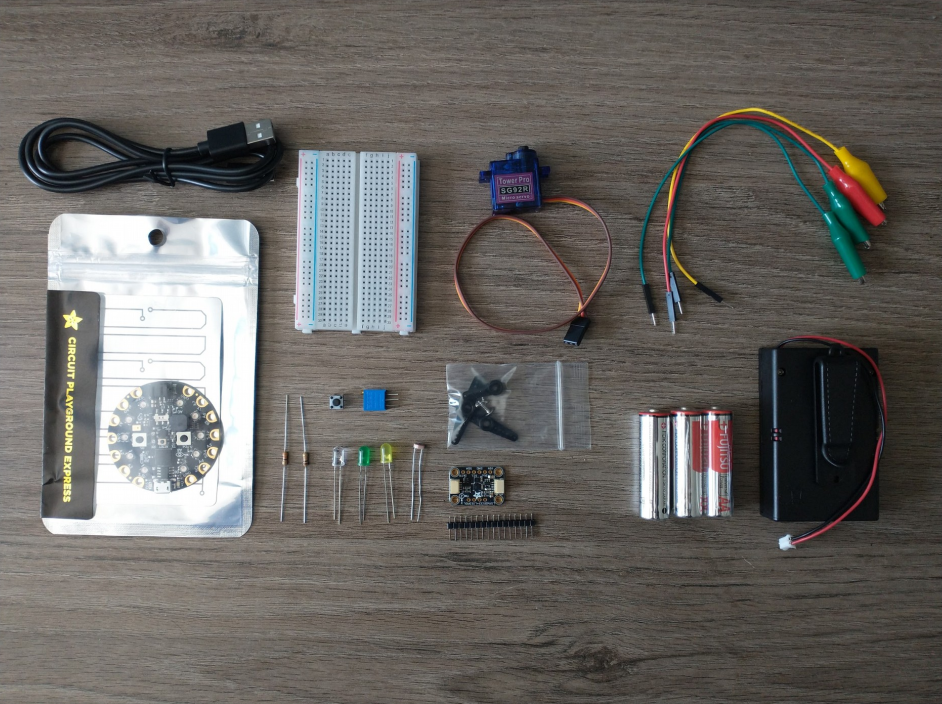
\includegraphics[width=0.8\textwidth]{Figures/components.png}
  \end{center}
\end{figure}

The CPX is a relatively new development board that operates in the
same style as Arduino\cite{Arduino}. That is, the student can
create a relatively simple script and then flash the software to the
CPX via USB. The Arduino operates in the same way. The benefit of the
CPX vs the Arduino is that the software is CircuitPython which is
indistinguishable from Python. As mentioned earlier, Python is in the
top 3 programming languages as stated by the Tiobe Index of
Programming\cite{Tiobe}. Other benefits include the components
built in to the CPX. The CPX itself contains a built in microphone,
accelerometer, light sensor, speaker, three push buttons, slide switch
and infrared sensor. The CircuitPlayground Express (CPX) also contains
10 smart NeoPixel LEDs and a ring of copper plated pads that can be
attached to the included alligator clips and breadboard. Students can
also elect to purchase the CircuitPlayground Bluefruit (CPB) which
does not have an infrared sensor but does contain bluetooth
functionality to send data wirelessly to the Adafruit Connect App
which runs on Apple/Android\cite{AdafruitBLE}.

\subsection{Assignment}
Your assignment for this module is to purchase the required equipment for your class. Note that the specific equipment will be instructor dependent so be sure you discuss with the instructor of your course before buying everything. At a minimum you must purchase a CPX or CPB but the rest of the items in your kit will depend on which modules your instructor wants you to do during the semester. {\bf Note that the CPX/CPB requires a microUSB cable and that cable must have a data line. Many USB cables are just power and ground.}

Once you've completed the project above, upload a PDF with all of the photos and text
below included. My recommendation is for you to create a Word document
and insert all the photos and text into the document. Then export the
Word document to a PDF. For videos I suggest uploading the videos to
Google Drive, turn on link sharing and include a link in your
PDF. Note that all code must be included in the appendix or you'll be
penalized 10\%. 


\begin{enumerate}[itemsep=-5pt]
\item A figure of your receipt of your purchases this semester - 80\%
\end{enumerate}

%\subsection{Quick Links}
%\begin{enumerate}[itemsep=-5pt]
%  \item \href{https://www.tangiblesthatteach.com/product-page/instrumentation-kit-for-me-316}{Kit}
%  \item \href{https://a2279211-28c1-4f46-9477-0d3265900c7f.filesusr.com/ugd/2413aa_ca39175b0a514b838ec96893b90590eb.pdf}{Document}
%  \item \href{https://youtu.be/6sNNQrhnzLE}{Unboxing Video}
%\end{enumerate}
%\subsection{Turning in this assignment}
%\begin{enumerate}[itemsep=-5pt]
%  \item Upload a receipt of ALL of your purchases - 50\%
%  \item Put your name and the names of your group members. If working
%    alone, tell me you are planning on working alone in the PDF you
%    upload. In times of COVID, everyone is working alone - 50\%
%\end{enumerate}
%% \newpage

%% \begin{center}\LARGE{ONLY READ BELOW IF YOU DON’T WANT TO BUY THE KIT
%%     ABOVE}\end{center}

%% \subsection{Purchase Items Yourself}

%% The bill of materials listed below is designed for 2 or 4 students to work together and share
%% pieces. This kit is not optimized for 3 students. If you are a remote/online student or you just
%% prefer to work alone then you have the option of purchasing everything yourself. The cost per
%% student in a group of 4 and 2 is listed as well as the cost if working alone. You’ll find that even
%% with the optional equipment, the cost of working alone is still less than the price of a standard
%% college textbook. Note that if you are working alone, be sure to only purchase 1 of each item. If
%% working in pairs you also have the option of purchasing one of each item. Finally, if you own
%% some of these components you may wish to simply purchase each item separately. A detailed
%% parts breakdown is shown after the rubric.

%% \subsection{Bill of Materials (per 4 students)}

%% \begin{figure}[H]
%%   \begin{center}
%%     \begin{tabular}{|l|c|c|}
%%       \hline
%%       Item (ONLY IF YOU DON’T WANT THE KIT ABOVE) & Quantity & Total
%%       Cost \\
%%       \hline
%%       \href{https://www.adafruit.com/product/3333}{Circuit Playground Express (CPX)} & 2 & \$50 \\
%%       \hline
%%       \href{https://www.adafruit.com/product/169}{Servo} & 2 & \$10 \\
%%       \hline
%%       \href{https://www.adafruit.com/product/592}{USB Cable} & 2 & \$6 \\
%%       \hline
%%       \href{https://www.amazon.com/Smraza-Breadboard-Resistors-Mega2560-Raspberry/dp/B01HRR7EBG/ref=sr_1_3?dchild=1&keywords=photocell+circuit+kit&qid=1590531716&sr=8-3}{Electronics Kit} (Photocells, Resistors, Trimpot) & 1 & \$13 \\
%%       \hline
%%       \href{https://www.amazon.com/WGGE-WG-026-Pieces-Colors-Alligator/dp/B06XX25HFX/ref=sr_1_1_sspa?dchild=1&keywords=alligator+clips&qid=1613147431&sr=8-1-spons&psc=1&spLa=ZW5jcnlwdGVkUXVhbGlmaWVyPUFLRjlYRVM3SDIySVAmZW5jcnlwdGVkSWQ9QTAwNDczMzEyODNCVTJWSjlMR0NEJmVuY3J5cHRlZEFkSWQ9QTAwMDQyMjkzSlJLNjJRWk9CSVZEJndpZGdldE5hbWU9c3BfYXRmJmFjdGlvbj1jbGlja1JlZGlyZWN0JmRvTm90TG9nQ2xpY2s9dHJ1ZQ==}{Alligator Clips} & 1 & \$4 \\
%%       \hline
%%       {\bf Total} & & {\bf \$83} \\
%%       \hline
%%       {\bf Cost per student in a group of 4} & & {\bf \$21} \\
%%       \hline
%%       {\bf Cost per student in a group of 2} & & {\bf \$25} \\
%%       \hline
%%       {\bf Cost if working alone} & & {\bf \$50} \\
%%       \hline
%%        & & \\
%%       \hline
%%       {\bf Optional Equipment} & & \\
%%       \hline
%%       \href{https://www.adafruit.com/product/3287}{External Power Supply} & 2 & \$6 \\
%%       \hline
%%       \href{https://www.adafruit.com/product/3349}{AA Batteries} & 2 & \$6 \\
%%       \hline
%%       \href{https://www.amazon.com/Hobbypower-Airspeed-MPXV7002DP-Differential-controller/dp/B00WSFWO36/ref=sr_1_3?dchild=1&keywords=Airspeed+sensor+kit&qid=1590532161&sr=8-3}{Analog Pitot Probe} & 1 & \$31 \\
%%       \hline
%%       \href{https://www.adafruit.com/product/4485}{Rate Gyro (LSM6D3SS)} & 1 & \$10 \\
%%       \hline
%%       & & \\
%%       \hline
%%       {\bf Total with Optional Equipment} & & {\bf \$136} \\
%%       \hline
%%       {\bf Cost per student in a group of 4} & & {\bf \$34} \\
%%       \hline
%%       {\bf Cost per student in a group of 2} & & {\bf \$50} \\
%%       \hline
%%       {\bf Cost if working alone} & & {\bf \$97} \\
%%       \hline
%%     \end{tabular}
%%   \end{center}
%% \end{figure}

%% \subsection{Detailed Parts List}

%% If you want to just purchase each component separately you can, just
%% make sure you have all of the parts below.

%% \begin{enumerate}[itemsep=-5pt]
%%   \item Circuit Playground Express (CPX)
%%   \item Servo
%%   \item Alligator Clips
%%   \item USB Cable
%%   \item Push Button
%%   \item Breadboard
%%   \item Photocell
%%   \item Resistors (10 kOhm, 330 Ohm, 1 kOhm)
%%   \item LED (x3 in case you fry one)
%%   \item Male to Male Wires (x2)
%%   \item Potentiometer
%% \end{enumerate}

%% You can also purchase some optional equipment as shown below.

%% \begin{enumerate}[itemsep=-5pt]
%% \item Rate Gyro (LSM6D3SS)
%% \item Male to Male Wires (x2)
%% \item Alligator Clips (x1)
%% \item Double Sided Tape
%% \item Analog Pitot Probe
%% \end{enumerate}

\newpage 

\section{Download Python for Desktop}

As you learn Instrumentation throughout the semester, you will be
tasked with creating computer programs on the Circuit Playground
Express (CPX). The CPX itself has it’s own RAM, CPU, HDD and many
sensors. Your CPX is kind of like a mini computer! You can plug the
CPX into your computer via USB and access the hard drive (HDD) from
your own computer. When you program on the CPX you need to write
programs on the CPX itself so that the mini computer can run the
program you wrote. The CPX knows how to read multiple different
languages but in this class we are going to write everything in the
\href{https://www.python.org/}{Python} language which has been ported
to the CPX and called
\href{https://circuitpython.org/}{CircuitPython}. Since we have to
write everything in CircuitPython we 
need to first learn how to program some things in Python. You can
easily download Python by itself but it’s nice to get what’s called an
Integrated Development Environment (IDE). This way you can practice
writing Python code on your computer while you wait for your purchases
to arrive in the mail. 

So which IDE can you download and which is recommended? I recommend
two IDEs. They are listed below. I recommend getting either one. If
you just Google “Python download” you will find a humongous list of
editors (Scratch, Anaconda, Canopy, Eclipse, PyDev, etc). It’s easy to
get lost when searching for something so broad. You’ve been warned.

\subsection{Thonny}

Thonny - \url{https://thonny.org/} -
\href{https://www.youtube.com/watch?v=qaxukpYRqfA&list=PL_D7_GvGz-v1RsDs_OdNW65qRjEjmpfQx&index=14}{Youtube
  video on how to install}

\begin{figure}[H]
  \begin{center}
    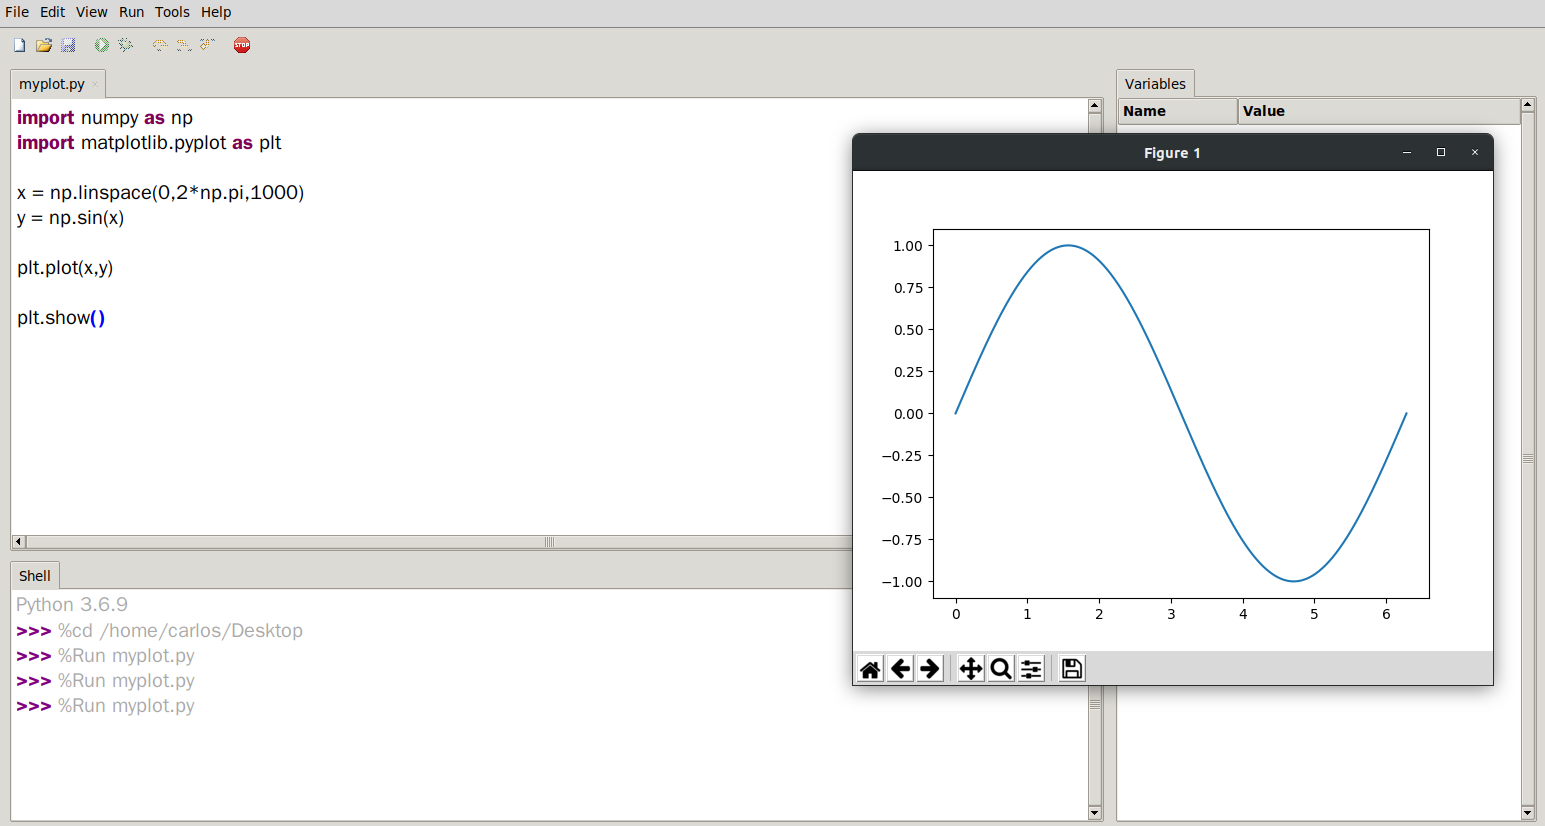
\includegraphics[width=\textwidth]{Figures/Thonny.png}
  \end{center}
\end{figure}

\subsection{Spyder}

Spyder - \url{https://www.spyder-ide.org/} - \href{https://www.youtube.com/watch?v=OjYwET-6QtE&list=PL_D7_GvGz-v1RsDs_OdNW65qRjEjmpfQx&index=35}{Youtube video on how to install}

\begin{figure}[H]
  \begin{center}
    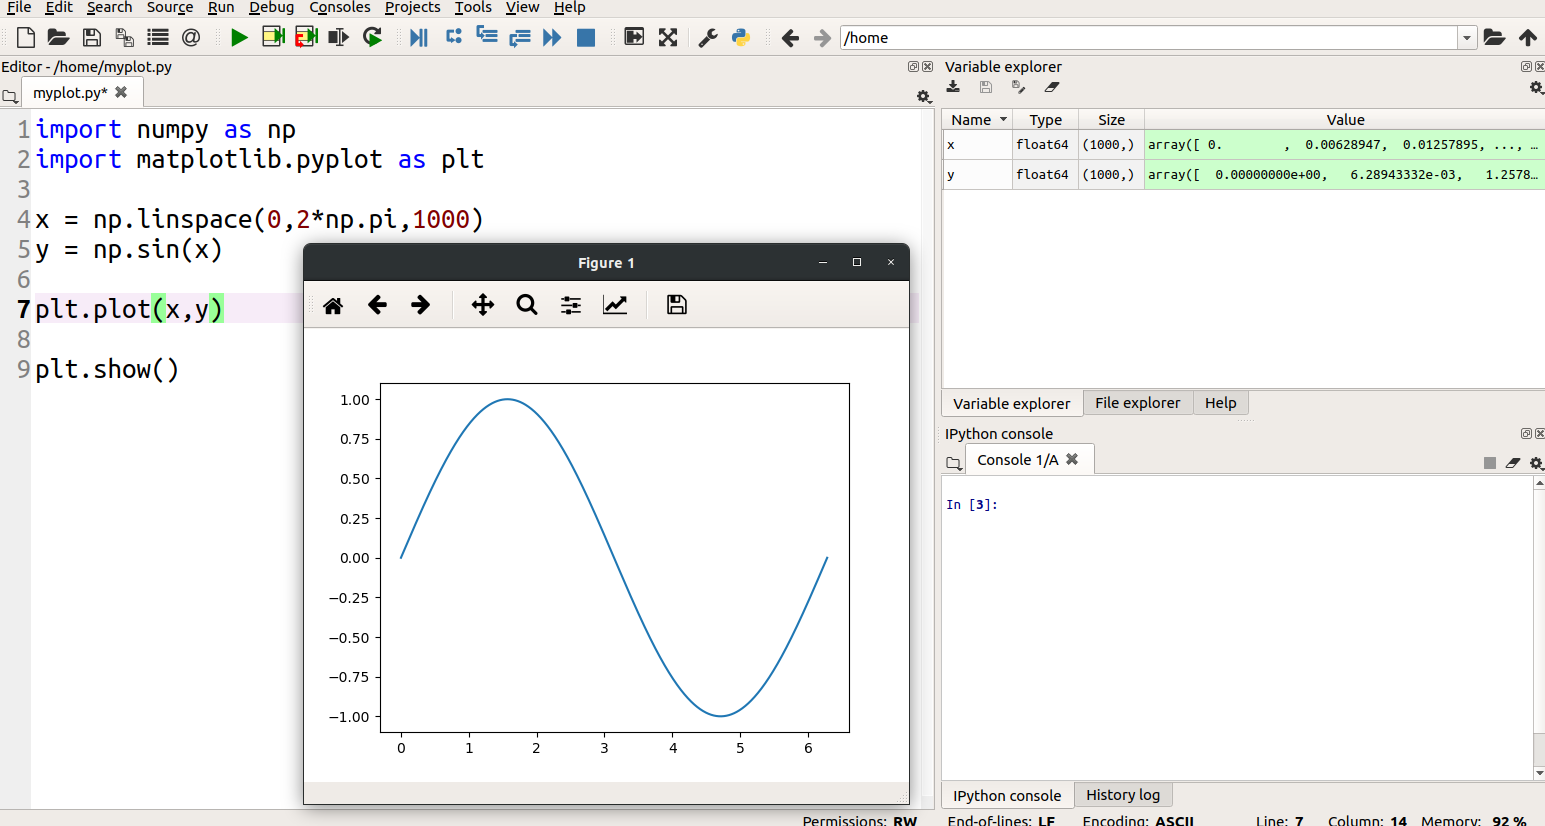
\includegraphics[width=\textwidth]{Figures/Spyder.png}
  \end{center}
\end{figure}

\subsection{Other Options}

It is possible to use
\href{https://colab.research.google.com/drive/1-VzSDojevQZ6A0oJNol9YXV6SRp3FKeP}{Google
  Colab} if you want to collaborate on Python projects or even get apps for your phone (\href{https://play.google.com/store/apps/details?id=ru.iiec.pydroid3&hl=en_US&gl=US}{Pydroid} or \href{https://apps.apple.com/us/app/pythonista-3/id1085978097}{Pythonista}
depending on Android or iPhone). You'll need to download 32 bit or 64
bit but which one? Well you need to figure out how many bits your
computer has. This is a great thing to Google. Type the following: "do
I have a 32 bit or 64 bit computer" into Google. I’m willing to bet
you have a 64 bit computer but you may as well check. We’ll learn
about the difference between 32 and 64 bit computers when we get to
the projects on Binary.

\subsection{Setting up your IDE}

Once you have Thonny or Spyder installed you need to install numpy and
matplotlib which are modules within Python that allow us to do some
extra things like numerical computation with Python (numpy) and Matlab
style Plotting libraries (matplotlib). I explain how to install
modules in my Youtube videos above; however, you need to head over to
Tools>Manage Packages in Thonny. You can see in the image below I
already have version 3.1.2 but I can upgrade to 3.2.2

\begin{figure}[H]
  \begin{center}
    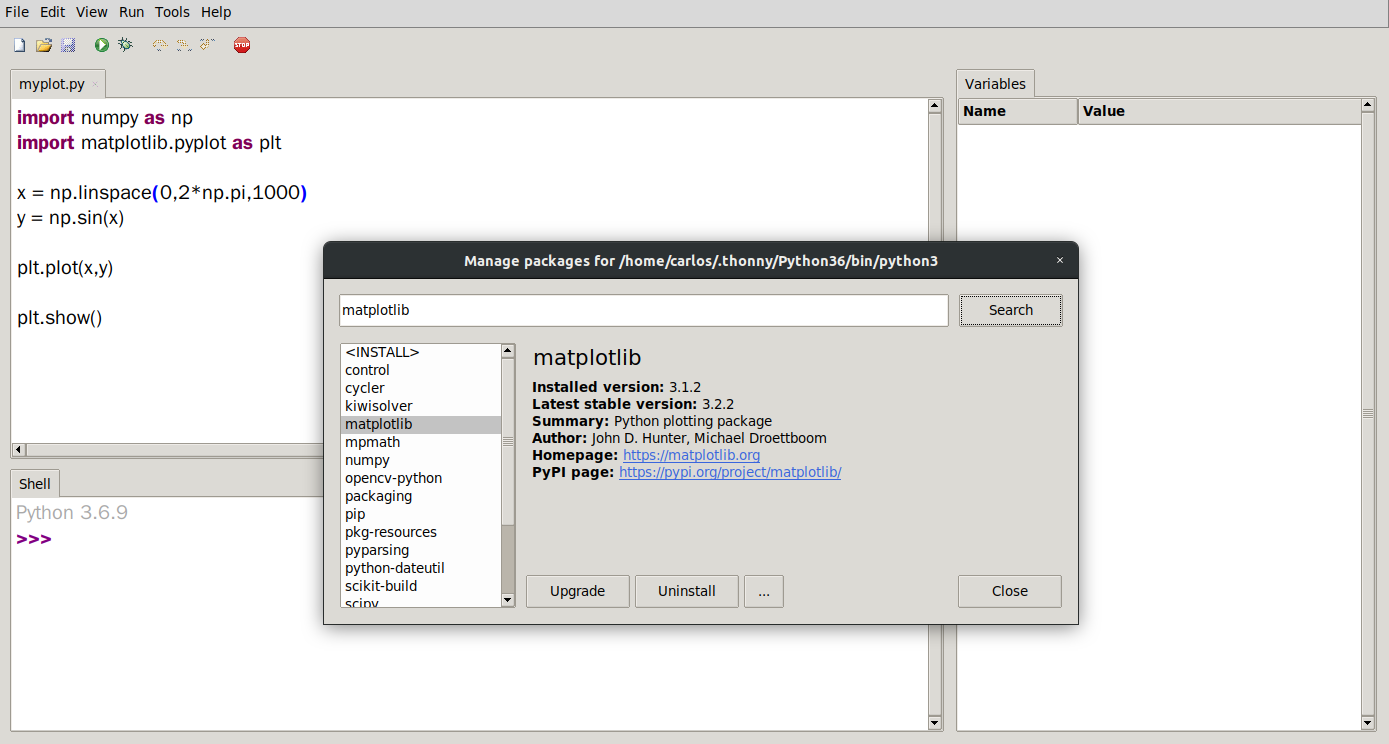
\includegraphics[width=\textwidth]{Figures/IDE_upgrades.png}
  \end{center}
\end{figure}

If numpy or matplotlib is not already included in Spyder then you need
to type the following into the Python Console in the lower right hand
corner of Spyder which is called the IPython console. 

\begin{verbatim}
!pip install matplotlib
\end{verbatim}

If that doesn’t work try

\begin{verbatim}
!pip3 install matplotlib
\end{verbatim}

You can see in the output example below that I already have matplotlib
installed as it says “requirement already satisfied”. Assuming you
have a valid internet connection it will install the necessary
module. 
\begin{figure}[H]
  \begin{center}
    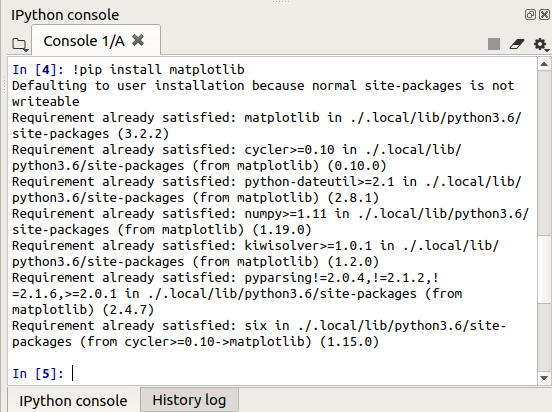
\includegraphics[width=0.5\textwidth]{Figures/console_thonny.png}
  \end{center}
\end{figure}

\subsection{Scripting}

Once you have numpy and matplotlib it’s time to make a plot. I have a
pretty \href{https://www.youtube.com/watch?v=7nAzHPURYW0&list=PL_D7_GvGz-v1RsDs_OdNW65qRjEjmpfQx&index=8}{comprehensive youtube video on how to plot in matplotlib} but if
you prefer text I will walk through a simple example.

\begin{figure}[H]
  \begin{center}
    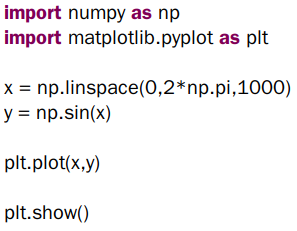
\includegraphics[width=0.5\textwidth]{Figures/matplotlib_example.png}
  \end{center}
\end{figure}

The code above will plot a sine wave from 0 to 2pi. The two lines at
the top are importing the numpy and matplotlib modules you installed
earlier. When they are imported we give them shorter names so it’s
easier to reference them so numpy will now be called np and
matplotlib.pyplot will be called plt. The next two lines then create a
vector “x” from 0 to 2pi using 1000 data points. The next line then
uses the sine function to create the vector “y”. Finally “x” and “y”
are plotted and the figure is instructed to pop up on your screen
using the show() function.


%% Now that you somewhat understand some of
%% this I’d like you to plot the following function: 

%% \begin{equation}
%%   T(t) = 60(1-e^{-5t})+30
%% \end{equation}

%% Plot the function from 0 to 10 seconds and label the x axis ‘Time
%% (sec)’ and the y-axis ‘Temperature (F)’. Add a grid as well. There are
%% some things that I have not explicitly shown you how to do. The reason
%% why is because I want to teach you how to fish for information.  

%% The first thing I recommend trying is to type in the commands in the
%% IPython console or the Shell. Type the first two commands below which
%% will show you every single function that numpy has available to you. 
%% \ \\

\subsection{Built-In Help Function and dir()}

Running code will always create syntax errors. Typing your syntax
error into Google will yield so many results you might get
lost. Sometimes it helps to know how to learn things just from your
computer. For example, type in the commands below in the IPython
console or the Shell.

\noindent {\it import numpy as np}\\
{\it dir(np)}
\ \\

\begin{figure}[H]
  \begin{center}
    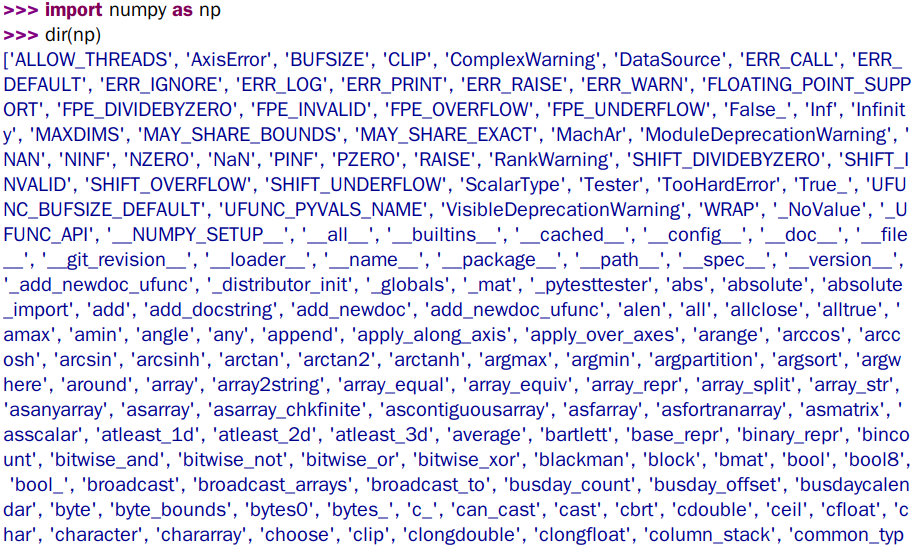
\includegraphics[width=\textwidth]{Figures/dir.png}
  \end{center}
\end{figure}

I included a photo of the output from the dir function. You’ll notice
there are a ton of functions in numpy. Every function in Python has a
\begin{verbatim} 
__doc__
\end{verbatim}

function. That’s two underscores followed by “doc” and then
another two underscores. If you’re ever curious about what a
particular function does you can just run the command below again in
the IPython console or Shell. In this example I’m looking at what
{\it arctan2} does.  

\begin{verbatim}
print(np.arctan2.__doc__)
\end{verbatim}

\begin{figure}[H]
  \begin{center}
    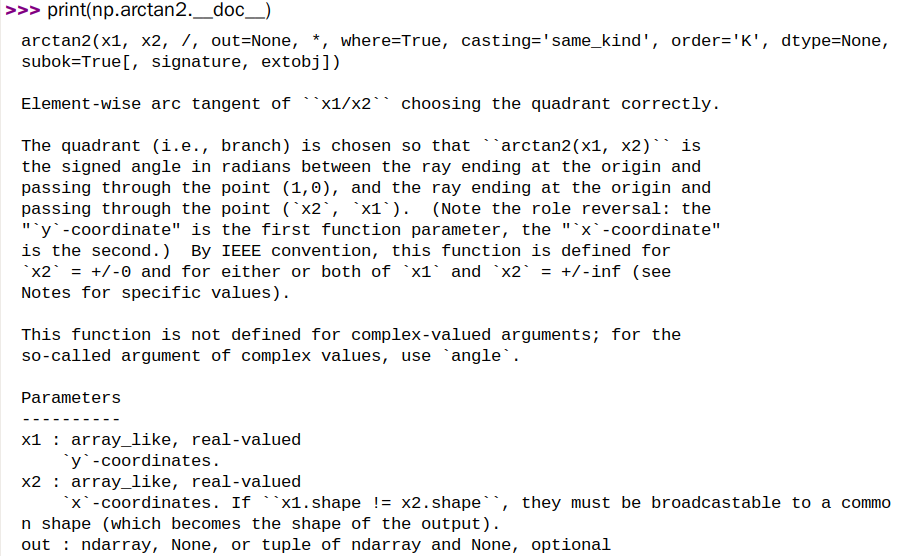
\includegraphics[width=\textwidth]{Figures/arctan2_doc.png}
  \end{center}
\end{figure}

You’ll see that arctan2 takes 2 input arguments “x1” and “x2”. I
didn’t include the entire output but if you continue to scroll through
the output it will even include examples on how to use the function.  

Another way to learn certain functions is by visiting the appropriate
documentation. The \href{https://numpy.org/doc/}{Numpy Docs} website
for example has all the documentation you need for Numpy. Navigating
that website you can find the same \href{https://numpy.org/doc/1.19/reference/generated/numpy.arctan2.html?highlight=arctan2#numpy.arctan2}{documentation for arctan2}.

As a last resort you can always Google “how to compute the inverse
tangent 2 function in Python”. Note though that there is so much
content out there on Google that you could easily get lost. Still,
there’s also so much information that the answers are out there for
just about anything.  

So you have three methods for finding out how to program in
python. The dir and {\it \_\_doc\_\_} functions in Python, using the appropriate
documentation online and of course Google. I’m lumping Youtube in with
Google which is also another way to learn information although when I
want to find information quickly I just use the documentation. It’s
the best in my opinion. 

\subsection{Assignment}

Your assignment for this project is to plot the equation below from 0 to 10 seconds and include that Figure in your report. You must add a grid and label the x-axis ‘Time (sec)’ and the y-axis ‘Temperature (F)’

\begin{equation}
  T(t) = 60(1-e^{-5t})+30
\end{equation}

Once you've completed the project above, upload a PDF with all of the photos and text
below included. My recommendation is for you to create a Word document
and insert all the photos and text into the document. Then export the
Word document to a PDF. For videos I suggest uploading the videos to
Google Drive, turn on link sharing and include a link in your
PDF. Note that all code must be included in the appendix or you'll be
penalized 10\%. 


\begin{enumerate}[itemsep=-5pt]
  \item Include a screenshot of your Python IDE (Thonny or Spyder is suggested) - 40\%
  \item Include the plot of temperature vs time being sure to save the figure so it is in high resolution - 40\%
\end{enumerate}


\section{Getting Started with the CPX/CPB}

\subsection{Parts List}
\begin{enumerate}[itemsep=-5pt]
  \item Laptop
  \item CPX(or CPB)
  \item USB Cable (with a data line. Not all USB cables have data
    lines)
\end{enumerate}

\subsection{Setting up your Circuit Playground}

By now you hopefully have your Circuit Playground (CPX) and it's time
to get your CPX up and running. A very in depth and detailed tutorial
can be found on the
\href{https://learn.adafruit.com/circuitpython-made-easy-on-circuit-playground-express/first-things-first}{Adafruit
  Learn site.} The text below is a summary 
of what you need to do to get the CPX up and running. 

When you get your CPX and plug it into the computer via USB it
actually won't run Python just yet. First you need to double click the
reset button (the button in the center. It says RESET above the
button) and put it into boot mode. All the neopixels (the ring lights
on the CPX) will light up green. 
\begin{figure}[H]
  \begin{center}
    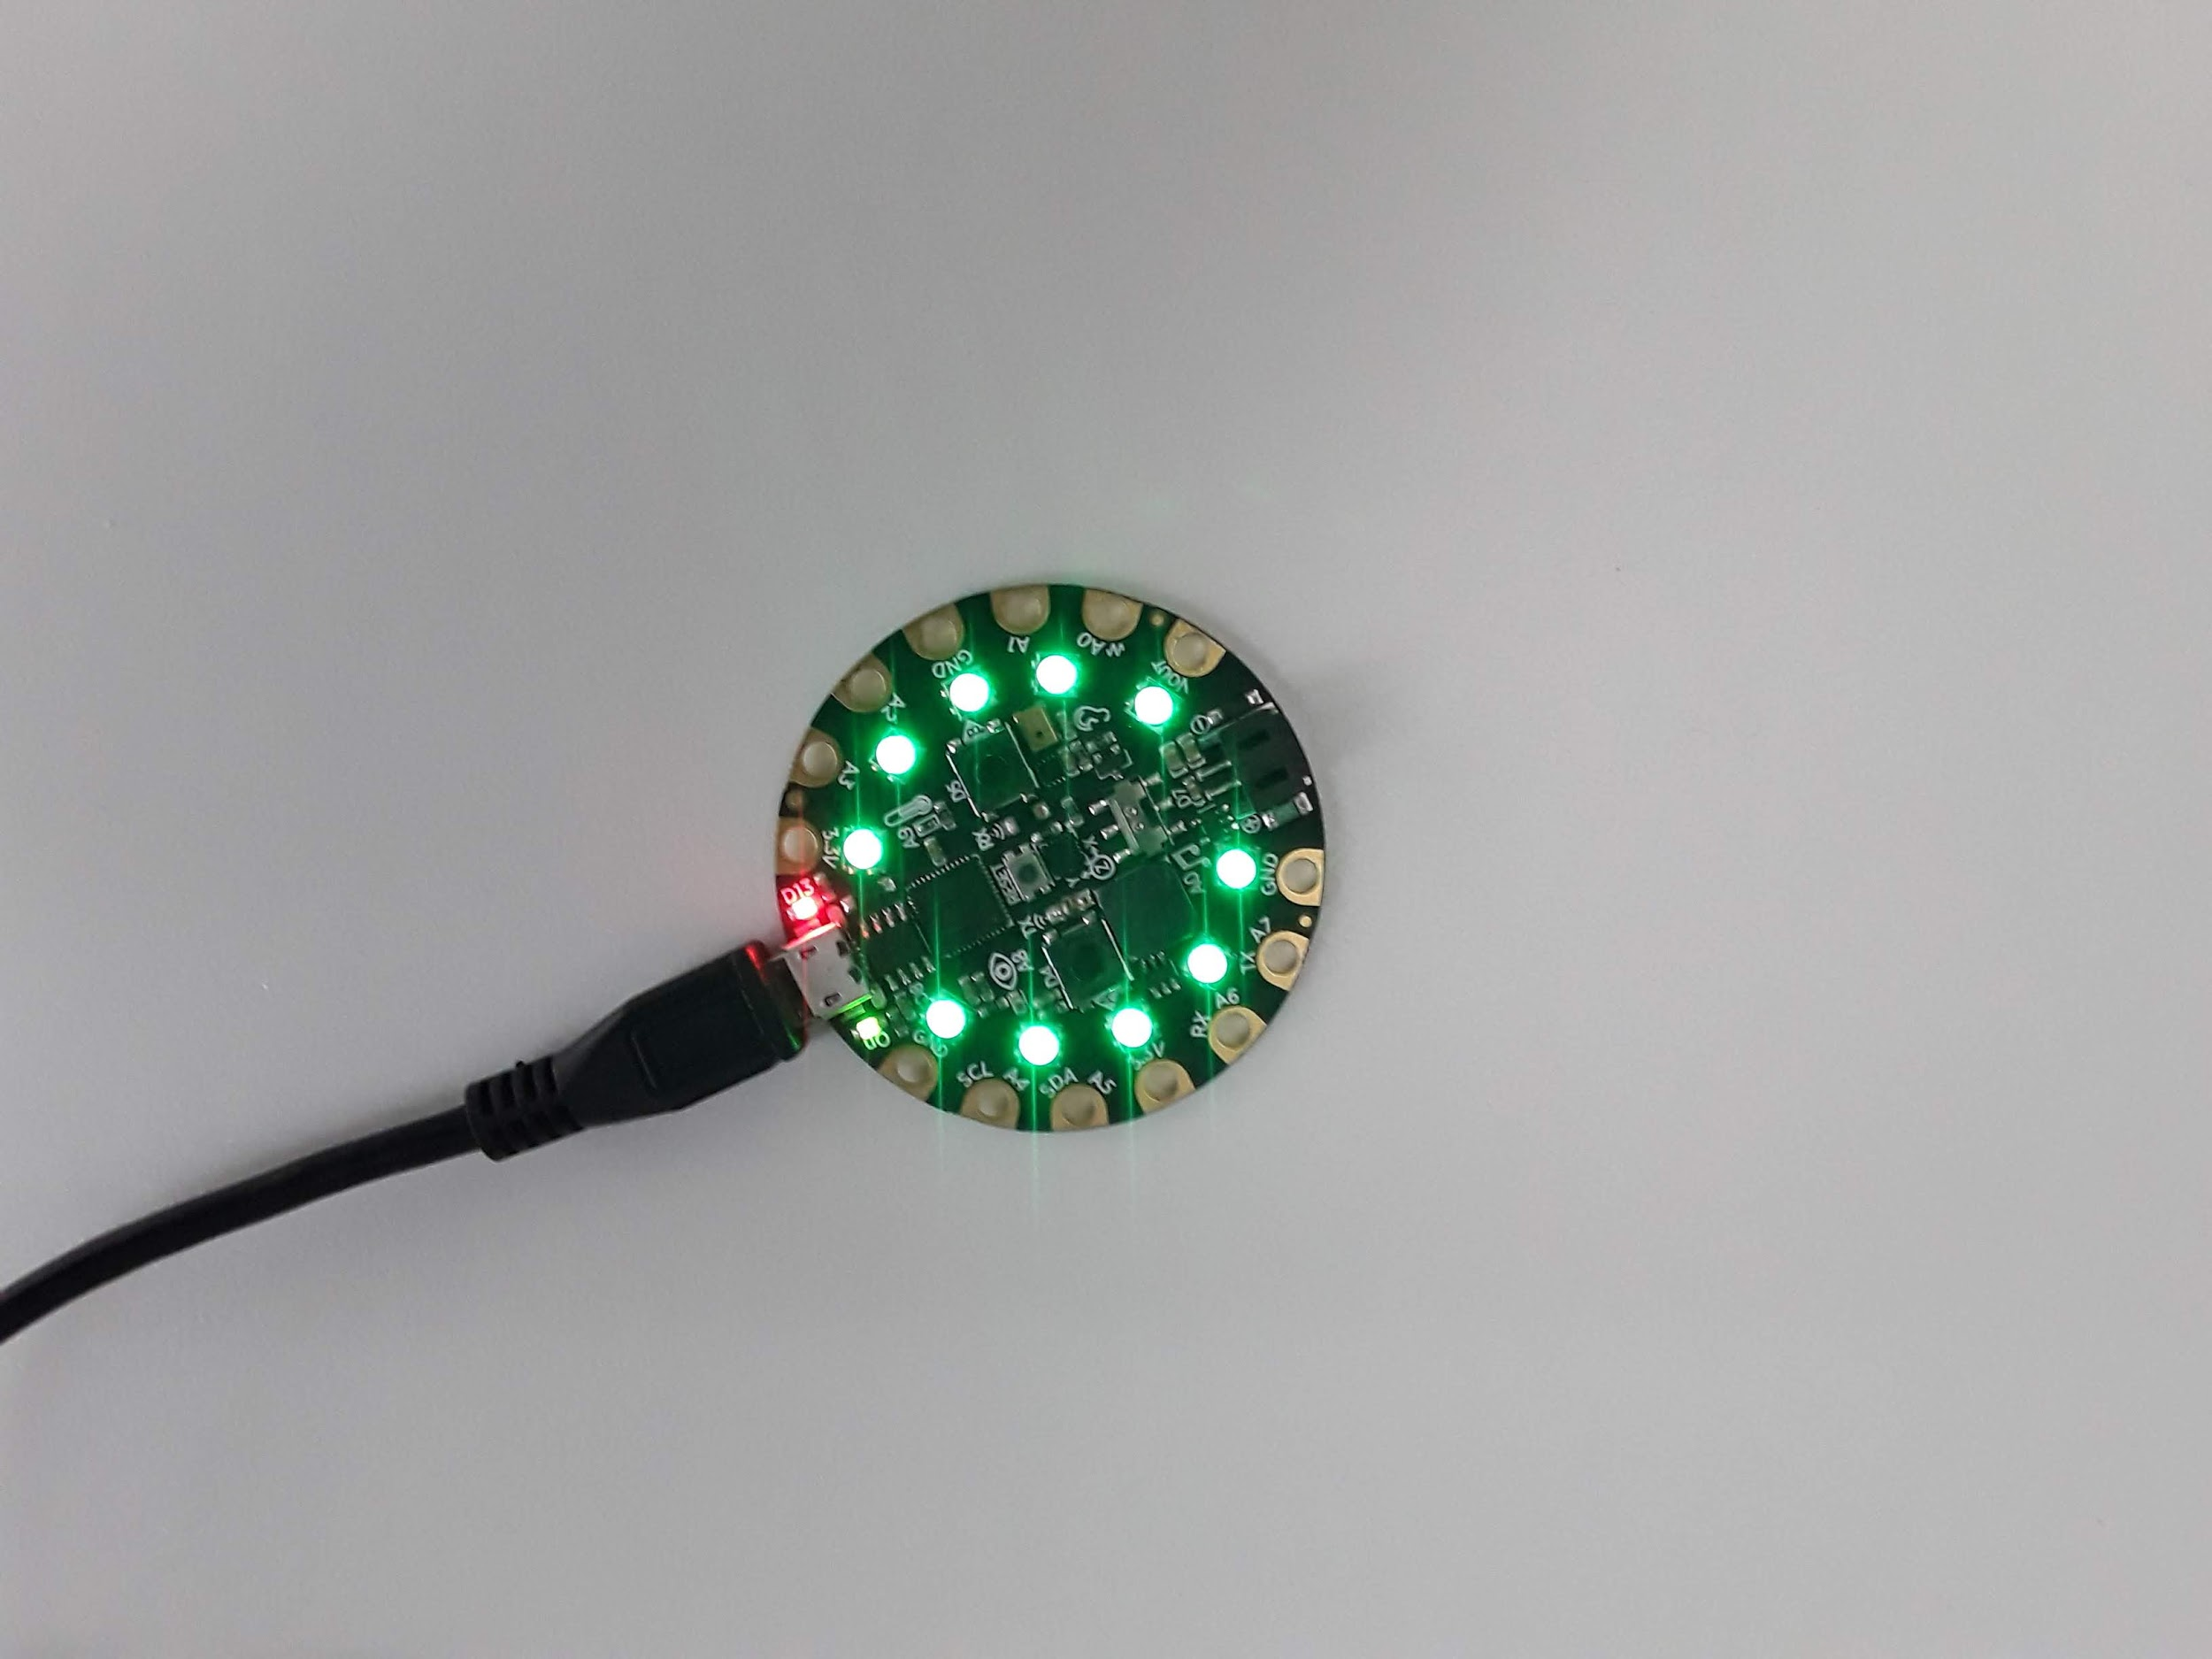
\includegraphics[width=\textwidth]{Figures/CPX_boot.jpeg}
  \end{center}
\end{figure}
Something called CPLAYBOOT will pop up on your computer just like a
USB stick or external harddrive. A couple files with be in there but
it doesn’t matter what they say right now.
\begin{figure}[H]
  \begin{center}
    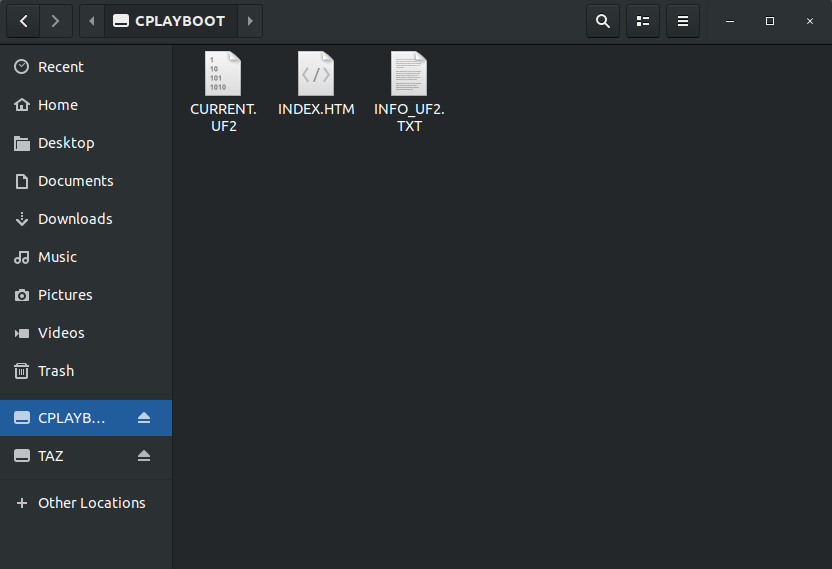
\includegraphics[width=\textwidth]{Figures/CPLAYBOOT.png}
  \end{center}
\end{figure}
You then need to download what’s called a \href{https://circuitpython.org/board/circuitplayground_express/}{UF2 file} and transfer it
onto the CPX. Note if you purchased a kit with the Bluefruit you need
to download a
\href{https://circuitpython.org/board/circuitplayground_bluefruit/}{different
  UF2}. Make sure you get the right one. Once the 
UF2 is downloaded you need to drag the UF2 over to the CPLAYBOOT drive
on your computer. After a bit of time a USB drive called CIRCUITPY
will pop up as a flash drive on your computer. The CPX is now like a
USB stick with 2MB of storage. 
\begin{figure}[H]
  \begin{center}
    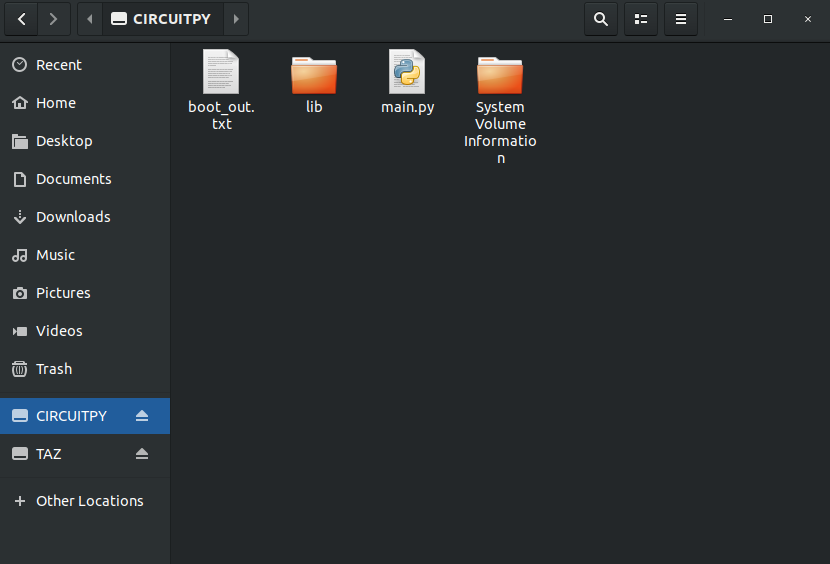
\includegraphics[width=\textwidth]{Figures/CIRCUITPY.png}
  \end{center}
\end{figure}
At this point the CPX is like a mini computer. If you put Python code
on the “flash drive” it will run python code. Since I’ve done this
before, there are a number of files already on my CPX. You may have
some or none of these. The “boot\_out.txt” file will tell you the
version of CircuitPython you have on the CPX. Mine says this:
\begin{verbatim}
Adafruit CircuitPython 5.3.0 on 2020-04-29; Adafruit CircuitPlayground Express with samd21g18
\end{verbatim}
Which means I have CircuitPython version 5.3.0 last updated on April
29th, 2020. The CPX itself is using the \href{https://www.microchip.com/wwwproducts/en/ATsamd21g18}{ATSAMD21G18}
microprocessor. The folder lib is a folder with extra libraries that
you may need to install later. The file main.py is the Python file
that the CPX is currently running. {\bf The CPX can store as many Python
files as possible for a 2MB flash drive but it will only run ONE
Python script at a time and that file must be named main.py} The folder
{\it System\_Volume\_Information} is a file management folder that we will
never use.

If you want the CPX to run code you simply need to edit the file
{\it main.py} or if that file does not exist you just need to create it. You
could just open Notepad or any other text app (Sublime,TexWrangler,
Emacs, Vi, Nano, Gedit, Notepad++, Wordpad, VSCode, etc) but the CPX
has alot of debugging options and it is recommended to use a program
called “\href{https://codewith.mu/en/download}{Mu}”. Mus is a good way to write and debug code on the
CPX. Note that Mu is only used to program the CPX. If you want to run
Python code on your laptop you need to use Thonny or Spyder (or
whatever other IDE you downloaded). If you want to run Python code on
your CPX you must use Mu. Once you’ve downloaded and installed Mu and
open it up it will look like this (Note it's possible the the software
gets updated from the time this book is published. As such be sure to
select the Circuitpython Mode for board development).
\begin{figure}[H]
  \begin{center}
    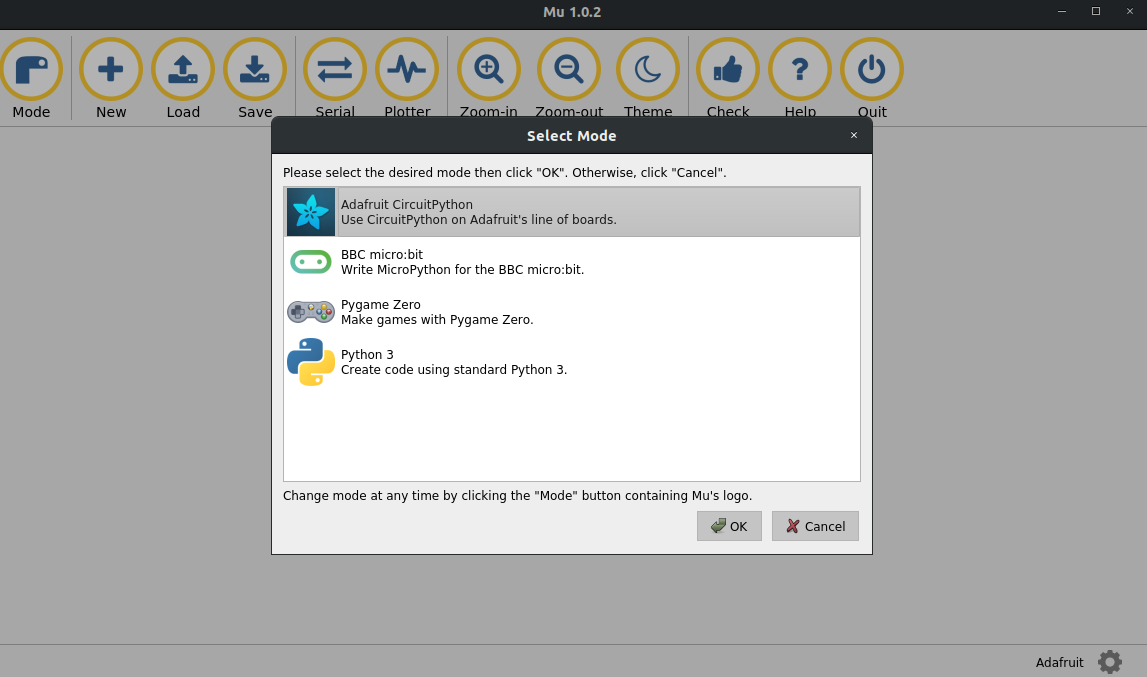
\includegraphics[width=\textwidth]{Figures/Mu.png}
  \end{center}
\end{figure}
Make sure to select the “Adafruit CircuitPython” option. If the
software has been updated and that option no longer exists, be sure to
select the option that says Circuitpython for board development.

Alright, let’s start writing code! If you have a file called {\it main.py}
on your CPX click the Load button and load {\it main.py} (make sure to load
the main.py that is stored on your CPX and not somewhere else on your
computer.) If a file {\it main.py} does not exist on your CPX simply click
the New button and then Save the file as {\it main.py} (again make sure you
save it to the CPX and not to your computer) 
\begin{figure}[H]
  \begin{center}
    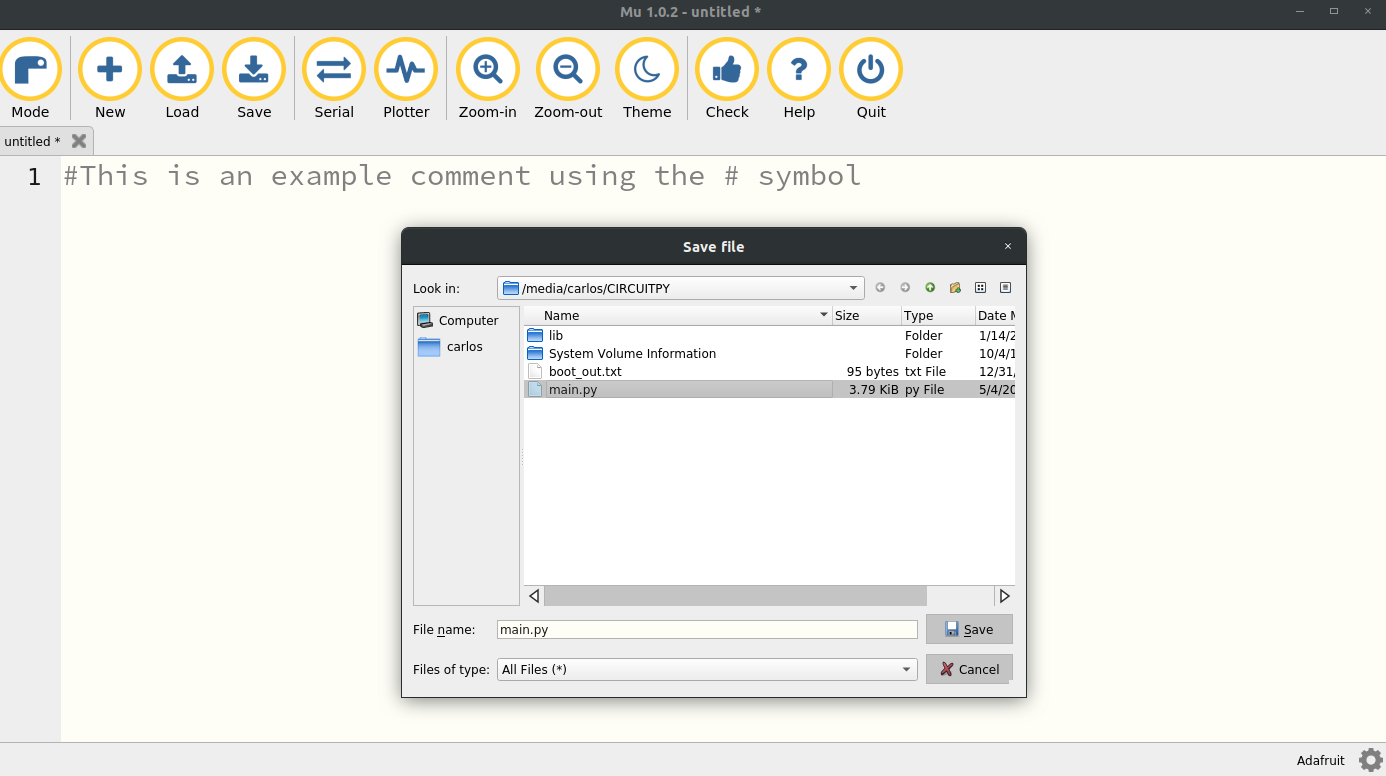
\includegraphics[width=\textwidth]{Figures/Mu2.png}
  \end{center}
\end{figure}
You’ll see that I am accessing the CIRCUITPY drive and saving the file
as main.py The file itself is empty and just has a comment using the \#
symbol. At this point since the file is blank the CPX won’t do
anything.

{\bf \it Now this is really important. Your CPX is a USB stick that can hold as
many Python files as 2MB will allow but it can only run or execute one
python script at a time. Furthermore it will only run two types of
files. It will run code.py if it exists and if it can't find code.py
it will run main.py If the CPX can't find main.py or code.y it will
just not do anything. If you have two versions of main.py or a
combination of main.py or code.py it will run one of them and not the
other. Make sure you only have one version of main.py or code.by but
not both! Some common things to check if your CPX isn't working. }
\begin{enumerate}[itemsep=-5pt]
  \item Make sure you're using Mu in the right Mode
  \item Make sure main.py or code.py is on the CIRCUITPY drive and not somewhere on your computer.
  \item Make sure you are editing the right file in Mu. Do you have two versions of main.py?
  \item Are you editing using Thonny or Spyder?
  \item Are you editing a file on your computer? Make sure you are writing to the CIRCUITPY drive.
  \item Unplug the CPX, close Mu and try again.
\end{enumerate}
So let’s get the CPX to do something simple like blink an LED. I have
an entire
\href{https://github.com/cmontalvo251/Microcontrollers}{Github}
devoted to Microelectronics. Specifically I have a
\href{https://github.com/cmontalvo251/Microcontrollers/tree/master/Circuit_Playground/CircuitPython}{folder
  with all of my Circuit Playground files}. The easiest program to 
run is the \href{https://github.com/cmontalvo251/Microcontrollers/blob/master/Circuit_Playground/CircuitPython/blink.py}{blink.py} script. I’ve attached a screenshot of the script
below. 
\begin{figure}[H]
  \begin{center}
    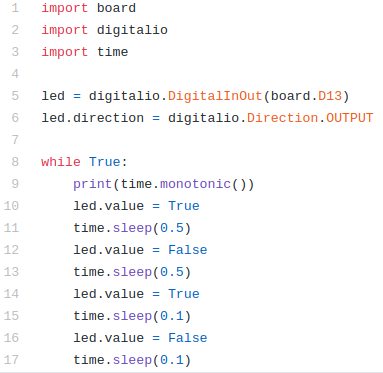
\includegraphics[width=\textwidth]{Figures/blink.png}
  \end{center}
\end{figure}
We will talk about what this code is doing later on. For now copy and
paste these 17 or so lines of code and paste them into Mu specifically
the {\it main.py} script. It will hopefully look like this.
\begin{figure}[H]
  \begin{center}
    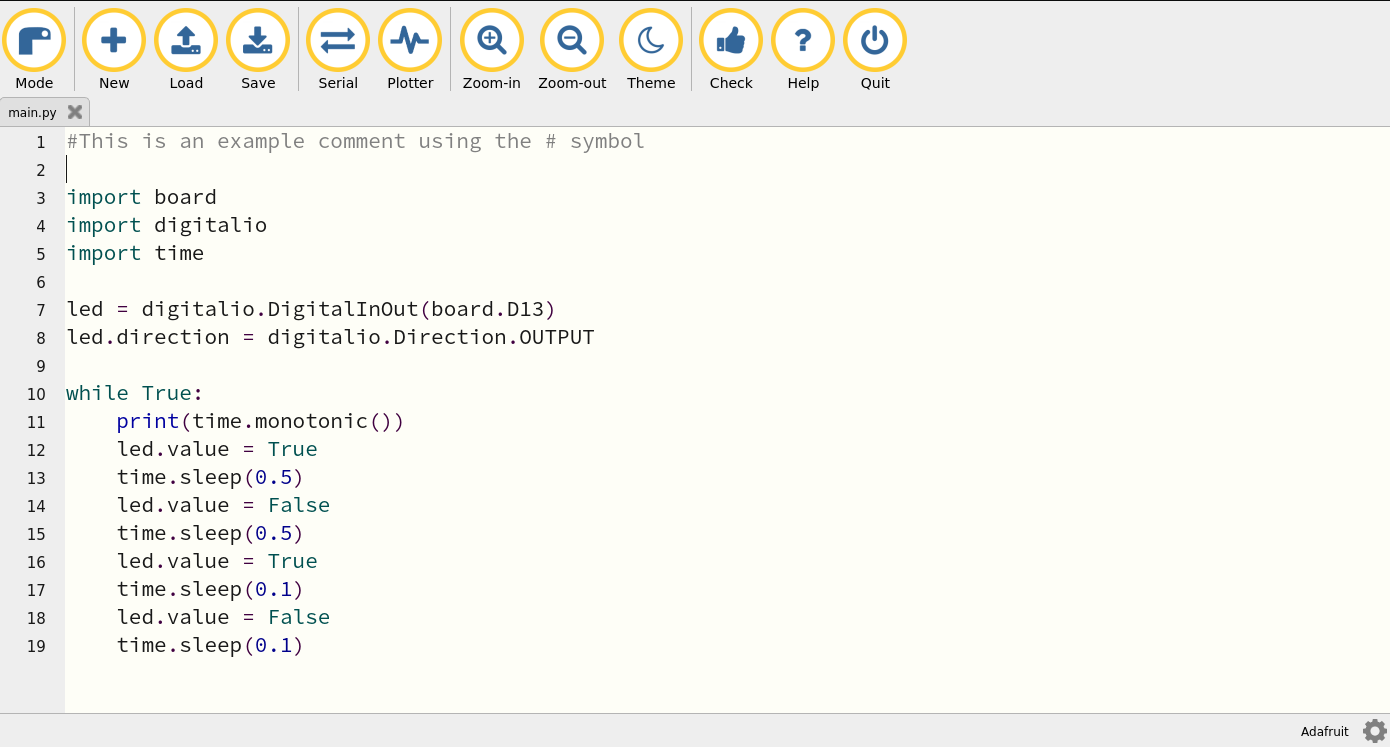
\includegraphics[width=\textwidth]{Figures/blinkmu.png}
  \end{center}
\end{figure}
Make sure to save. You can click {\it Zoom-In} and {\it Zoom-out} to zoom in and
out to change the font size and see more of the output. If the blink
code is working you will see a red led labeled D13 on the CPX blink
back and forth. D13 stands for digital pin 13. You’ll notice there are
analog pins labeled A5 and A6 among other numbers. Let’s talk about
the code a bit more and explain why it’s doing what it’s doing. The
three lines at the top of the code are {\it import} commands to import
different modules just like we did for {\it numpy} and {\it matplotlib}. In this
case the modules being imported are {\it board}, {\it digitalio} and
{\it time}. The module {\it board} is used to import the layout of the
CPX so we can access different pins on the CPX. The module {\it digitalio}
stands for digital input output which means we are inputting and
outputting digital signals. Since we can combine this module with the
{\it board} module we will be able to output digital signals to
different pins on the CPX board. Remember that PCB stands for printed
circuit board so {\it board} implies we are accessing pins on the CPX
PCB. Hopefully that makes sense. The final module we are importing is
{\it time} which acts just like the {\it time} module on your desktop
computer. It will let us access the CPX’s internal clock.

Moving along, lines 7 and 8 create an LED object using the {\it board}
module and {\it digitalio}. It’s a long line of code that basically says,
create a variable called {\it led} that lets us output a digital signal to
pin D13. We also set the direction of the LED to output since we only
want to write to the LED.

Lines 10 through 19 kick off an infinite loop that never ends. The
line that says {\it while True:} means loop while {\it True}. Well
{\it True} is always true which means it will loop forever. The colon
at the end of the line tells Python that the loop condition statement
ends and to begin looping from 11 through 19.

Line 11 specifically says {\it print(time.monotonic())}. First the
{\it print()} function is used to print things so that you and I can
see it. Rather than just seeing a blinking LED we want to see the time
printed. The {\it time.monotonic()} is using the module {\it time} which we
imported and using a function from that module called {\it monotonic()}
which calls the internal clock of the CPX. So how do you see the
output from the print statement? Hit the {\it Serial} button on Mu and you
will hopefully see some output. Here’s what it looks like on my
machine. 
\begin{figure}[H]
  \begin{center}
    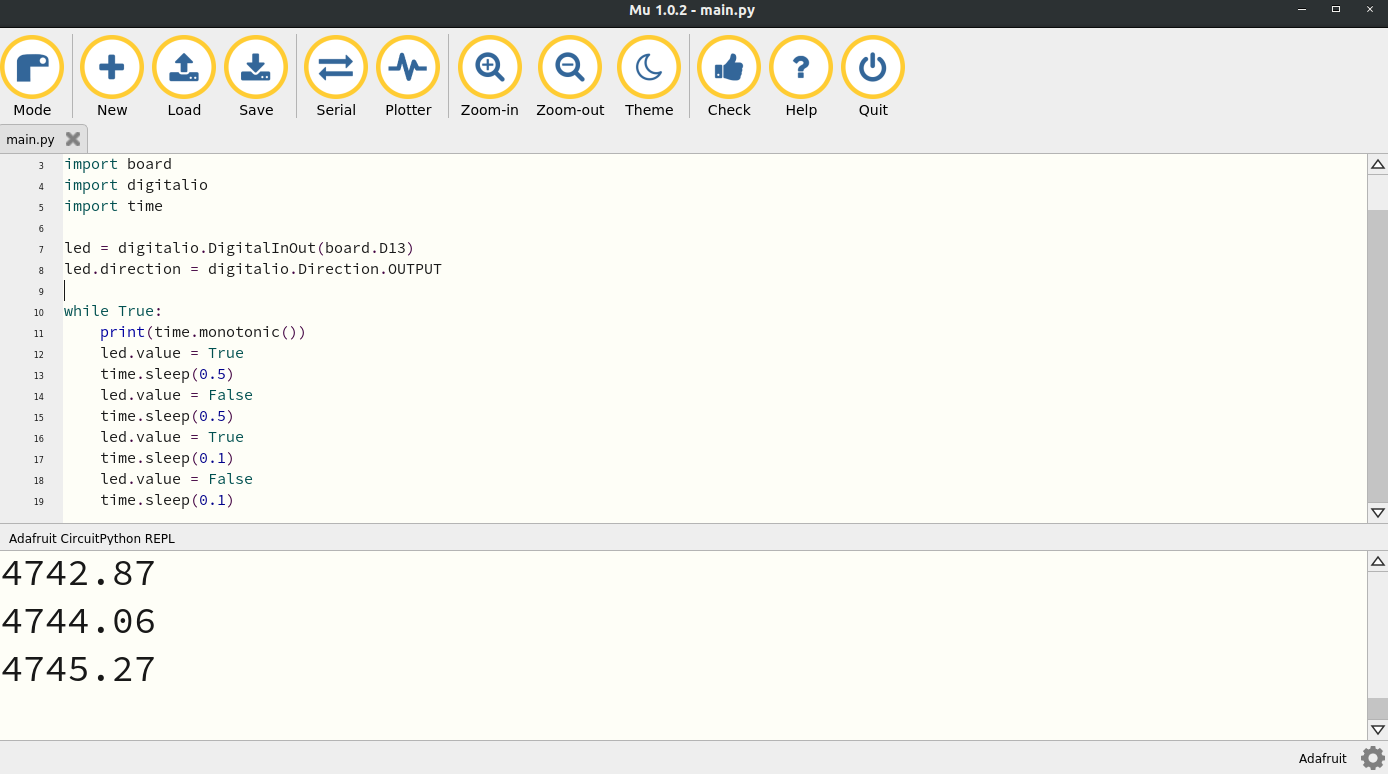
\includegraphics[width=\textwidth]{Figures/blinkmu2.png}
  \end{center}
\end{figure}
In this case you can see the time printed every time it goes through
the loop. You may even see an error. This {\it Serial} button is great for
debugging because it will tell you the error in your code. For
example, in the picture below I have an error in my code and the
{\it Serial} output is letting me know.
\begin{figure}[H]
  \begin{center}
    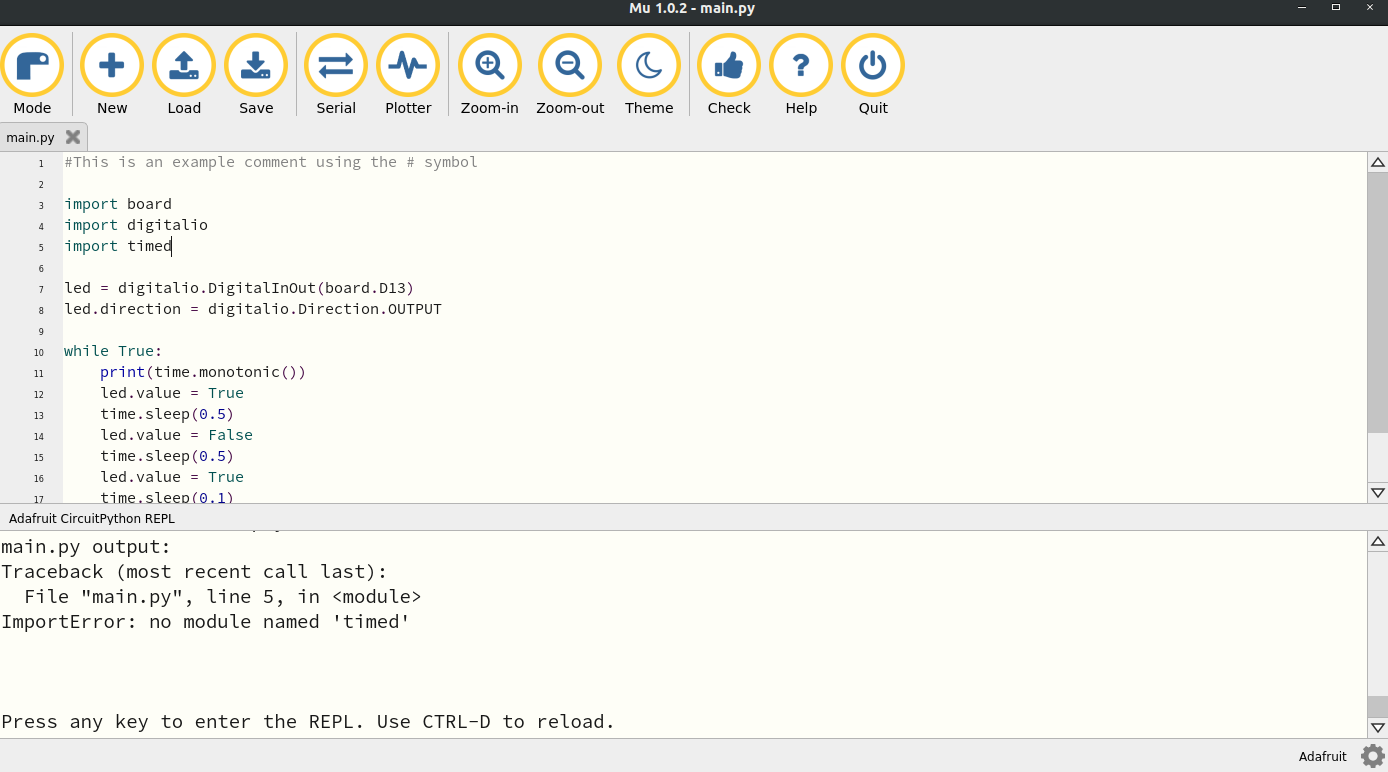
\includegraphics[width=\textwidth]{Figures/blinkerror.png}
  \end{center}
\end{figure}
In this case I have an error on line 5. It’s saying there is no module
named {\it timed}. The reason that module doesn’t exist is because the
module is actually {\it time} not {\it timed}. You can use the {\it
  Serial} monitor to check on your program and see what errors you may
have. Ok so there are two more lines of code to discuss. They are
{\it led.value = True} and {\it time.sleep(0.5)}.

These lines of code are repeated throughout the while loop and do two
things. First, the {\it led.value} either sets the value of the LED to
True which turns the light on or False which turns the light off. The
LED is digital which means the signal can either be on or off. There’s
no in between for digital signals. The {\it time.sleep()} function
tells the CPX to pause for half a second. You can change the number in
the parentheses if you want to change length of time the code
pauses. Note that the CPX completely pauses. That is no code runs
during a sleep.

If you’ve gotten the LED to blink you’re all set for this
lab. However, I’d like to you learn a few more things about
documentation. Just like Python on your desktop you can lookup the
documentation on the CPX itself. For example, I’ve added a print
statement to print the directory of time.
\begin{figure}[H]
  \begin{center}
    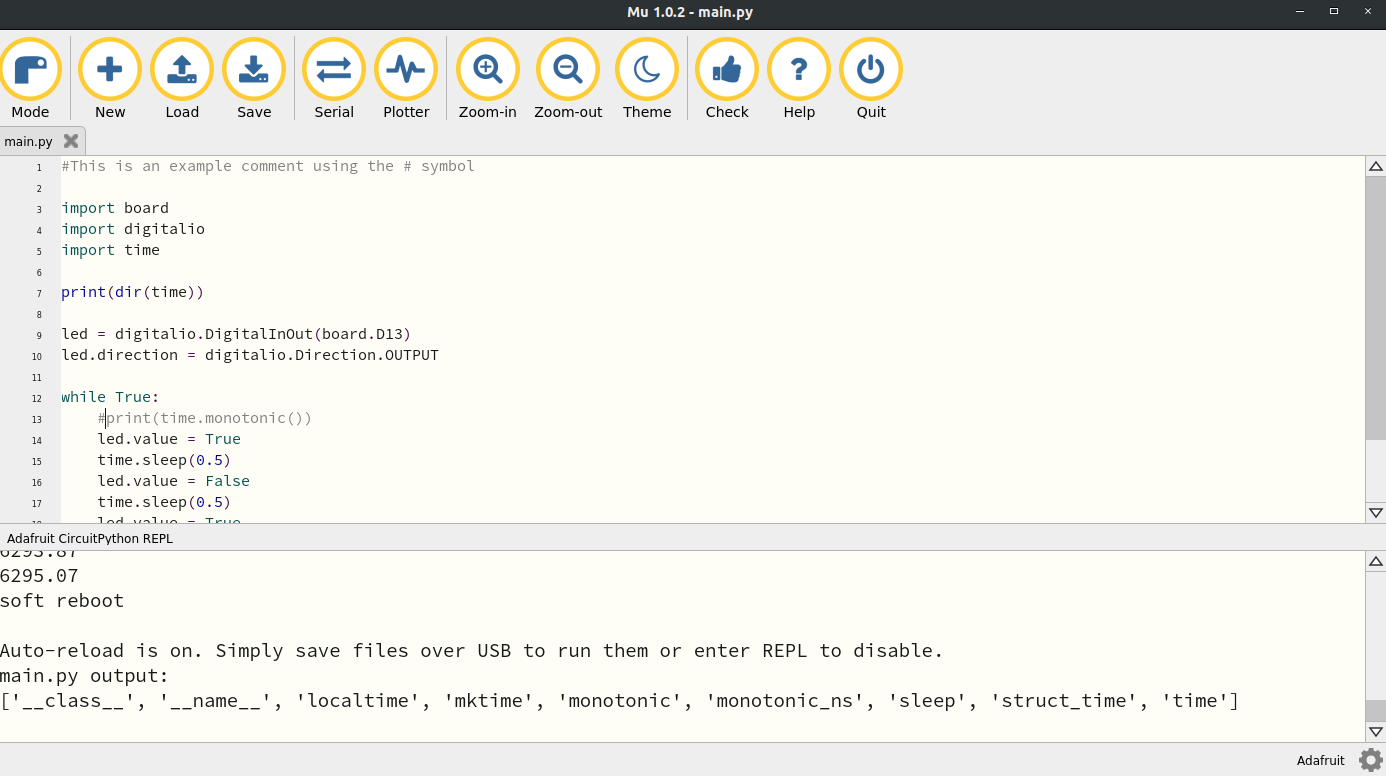
\includegraphics[width=\textwidth]{Figures/printtimeMu.png}
  \end{center}
\end{figure}
In this case I’ve added {\it print(dir(time))} to line 7. The output shows
that the {\it time} module has 9 functions including
{\it monotonic()}. Unfortunately CircuitPython does not have {\it \_\_doc\_\_}
functions built in which means if you want to learn about a specific
function, you need to visit the \href{https://circuitpython.readthedocs.io/en/5.3.x/README.html}{documentation for
CircuitPython}. Here’s the \href{https://circuitpython.readthedocs.io/en/latest/shared-bindings/time/index.html}{specific documentation for the} \href{https://circuitpython.readthedocs.io/en/latest/shared-bindings/time/index.html}{time}
\href{https://circuitpython.readthedocs.io/en/latest/shared-bindings/time/index.html}{module}. A lot of \href{https://github.com/adafruit/Adafruit_Learning_System_Guides/tree/master/CircuitPython_Essentials}{example code from the Adafruit Learning System is
also on Github.}

Finally, in order to keep practicing using Python on your desktop I
want you to modify the code above to run on your desktop
computer. You’re going to have to modify a few things. First, make
sure to open Thonny or Spyder depending on which version of Python IDE
you downloaded. Then, only import the {\it time} module. All the other
modules don’t exist on your desktop. Also, get rid of all the lines of
code that blink the LED. We just want to print time in a while
loop. Finally, the time module on your desktop uses a function called
time.time() (unless you have Python3 installed) so when you print time
make sure to use that module instead. Again visit the \href{https://docs.python.org/3/library/time.html#functions}{documentation
for time for Python if you want to learn more}. Thonny by default will
load Python version 3 but it’s possible you may have Python version 2
so make sure you look up the documentation for the appropriate version
of Python. After searching through the documentation you can use a
function called asctime() on your desktop. This is the output I get in
Thonny when I add a sleep of 1 second. The exercise for you is to do
something similar. 
\begin{figure}[H]
  \begin{center}
    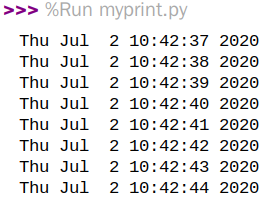
\includegraphics[width=\textwidth]{Figures/blinkcomputer.png}
  \end{center}
\end{figure}
\subsection{TL;DR}

\begin{enumerate}[itemsep=-5pt]
\item Plug in your CPX and double tap it to go into reset
  mode. CPLAYBOOT will mount to your computer. 
\item Download the \href{https://circuitpython.org/downloads}{UF2
  file}.
\item Drag the UF2 file to your CPLAYBOOT drive. After a few seconds
  CIRCUITPY will mount.
\item You need to then download
  \href{https://codewith.mu/en/download}{Mu}
\item Open Mu and make sure to select the mode Adafruit CircuitPython
\item Open main.py in Mu from the CIRCUITPY drive in Mu.
\item If code.py is on your CPX delete it
\item Copy the blink.py script into main.py
\item Once you have the script running, modify the script to run on
  your Desktop using Spyder or Thonny
\end{enumerate}

There is an accompanying
\href{https://www.youtube.com/watch?v=XFvLn6rwm3I}{youtube video to
  help you see me perform the 8 steps above.}

\subsection{Assignment}

Upload a PDF with all of the photos and text below included. My
recommendation is for you to create a Word document and insert all the
photos and text into the document. Then export the Word document to a
PDF. For videos I suggest uploading the videos to Google Drive, turn
on link sharing and include a link in your PDF.

\begin{enumerate}[itemsep=-5pt]
\item Include a screenshot of your computer showing the CIRCUITPY drive on your computer - 25\%
\item Copy and paste your blink.py code and write a paragraph explaining any changes you made to get it to work - 25\%
\item Take a video of you and your CPX blinking the LED. State your name, wave at the camera and show the CPX blinking (You must use software like OBS studio which records your screen and yourself. No cell phone videos allowed). - 25\%
\item Modify the blink.py code to run on your desktop computer in
  Spyder or Thonny. Copy and paste your desktop version of the code
  and screenshot the output. Include the code and the output in your
  submission - 25\%
\end{enumerate}


\section{Troubleshooting Guide}

{\bf Is your CPX/CPB broken or not running code? Read below.}

\begin{enumerate}[itemsep=-5pt]
  \item Your CPX is a USB stick that can hold as many Python files as 2MB will allow but it can only run or execute one python script at a time. It will look for code.py and then main.py and that's it. 
  \item Make sure you're using Mu in the right Mode (CircuitPython)
  \item Make sure main.py or code.py is on the CIRCUITPY drive and not somewhere on your computer.
  \item Make sure you are editing the right file in Mu. Do you have two versions of main.py or perhaps main.py and code.py?
  \item Do you have boot.py on there when you don't need it?
  \item Are you editing using Thonny or Spyder? You're supposed to use Mu. 
  \item Are you editing a file on your computer? Make sure you are
    writing to the CIRCUITPY drive.
  \item Do you have the right modules in your {\it lib} folder?
  \item Unplug the CPX, close Mu and try again.
  \item First, try and reset the CPX to CPLAYBOOT and reflash the UF2 to see if that fixes it.
  \item If you have a linux computer you can ``sudo screen /dev/ttyACM0" and then run ``import storage" and then ``storage.erase\_filesystem()"
  \item If that doesn’t work sometimes you just need to completely erase the CIRCUITPY drive so head over to this \href{https://learn.adafruit.com/adafruit-circuit-playground-express/troubleshooting}{troubleshooting guide} and follow some of the steps they tell you.
  \item As a last resort you can try to download these UF2s and
    hopefully it will fix all errors and mistakes -
    \href{https://cdn-learn.adafruit.com/assets/assets/000/048/745/original/flash_erase_express.ino.circuitplay.uf2?1512152080}{CPX}, \href{https://cdn-learn.adafruit.com/assets/assets/000/082/950/original/CP_Bluefruit_QSPI_Erase.UF2?1572026649}{CPB}
  \item If you're having an issue with an old bootloader be sure to update the \href{https://learn.adafruit.com/adafruit-circuit-playground-bluefruit/update-bootloader-use-command-line}{bootloader}. At the time of this writing here is the command you need to upload the new bootloader {\it adafruit-nrfutil --verbose dfu serial --package feather\_nrf52840\_express\_bootloader-0.8.0\_s140\_6.1.1.zip -p /dev/ttyACM0 -b 115200 --singlebank --touch 1200}. Note that the -- is a double dash and - is just one dash. Also this is for the feather\_nrf52840. You need to download the zip specific for the CPB by clicking the bootloader link. 
  \item Are you running out of memory? To figure out how much RAM you have on your CPX/CPB you need to {\it import gc} then run {\it gc.collect()} and then {\it print(gc.mem\_free())}. At the time of this writing, the CPX has about 17 KB of RAM and the CPB has around 140 KB of RAM. 
\end{enumerate}


\section{External LEDs and Push Buttons}

\subsection{Parts List}


\begin{enumerate}[itemsep=-5pt]
  \item Laptop
  \item CPX + USB Cable
  \item 2 Alligator clips
  \item Push Button
  \item Breadboard
  \item LED (Light Emitting Diode) (x3 in case you fry some)
  \item Resistor (300 to 1000 Ohms)
\end{enumerate}

\subsection{Learning Objectives}

\begin{enumerate}[itemsep=-5pt]
\item The VOUT and 3.3V pin are always "ON" even when code is not
  running on the CPX. So long as your CPX is plugged in via USB or a
  Lipo Battery
\item LED are Light Emitting {\bf Diodes} which means current only flows in one direction
\item LEDs need resistors in series otherwise they will get too hot and burn up
\item Breadboard pinout diagrams
\item Analog pins can be controlled by simply using the digitalio module
\item LEDs can be hooked up to analog pins and set to blink by changing the board pin
\end{enumerate}

In this project we’re going to use the same blink code as before but
modify it to blink an external LED. The purpose of this lab is to
familiarize yourself with the pins on the CPX and create a simple
circuit using the 5V pin on the CPX and one of the Analog pins. Your
laptop has a battery with something between 10 to 20V. There are DC to
DC converters in your laptop that provide 5V to your USB ports. These
USB ports can be used to power your CPX as you have done in the past
few labs.

If you purchased the optional
\href{https://www.adafruit.com/product/3287}{battery pack} you can
also power the CPX using 3 AA batteries. These batteries nominally
have 1.5 V but fully 
charged it's actually something like 1.8 V. So 1.8 times 3 is 5.4V
which is enough to power the CPX. If you have the battery pack and
some AA batteries, give it a try. If you still have the blink code
from the last project on board you’ll see the D13 LED blink as
before. You won’t be able to see the serial print() output as before
but that code will be running which is why D13 is blinking. {\bf I have
noticed that some of the battery packs have power and ground wires
swapped. If the battery pack doesn’t work it may be because those two
wires are backwards.}

The CPX itself uses 3.3V logic which means when it converts numbers to
binary a 0 (False) represents 0 volts and a 1 (True) represents
3.3V. The CPX has ports that are labeled various things. GND stands
for ground and you need to hook the negative end of your circuit to
this and it also has VOUT which supplies 5V to any circuit you
build. Hook the positive end of your circuit to the VOUT pin. There is
also a port labeled 3.3V and obviously that outputs 3.3V

You’re going to need to use a breadboard so if you’re not familiar
with how breadboards work I would recommend watching this \href{https://www.youtube.com/watch?v=mE33WpRWrXs}{video on how
breadboards work}. Your lab today specifically involves an external
LED. You can read about
\href{https://learn.sparkfun.com/tutorials/light-emitting-diodes-leds/}{LEDs}
more online if you wish. {\bf Remember that the long leg of the LED is 
the positive end and the short leg is the negative end.} The task today
is to wire an LED up to the CPX in the following ways

{\bf Whenever you modify a circuit on the breadboard, always be sure
  to remove power from the CPX. You can damage multiple components if
  you’re not careful.}

\subsection{LED with no Code}

For this part we are going to light up the LED without the use of any
code on the CPX. First, wire up the circuit with the positive end
connected to 5V. This is how my circuit looks. Make sure to use a
resistor between 300 and 1000 Ohms. An LED does not have that much
internal resistance so you need a resistor in series with an LED to
reduce the amount of current flowing through the LED or the entire LED
will fry. If you use a resistor that has too much impedance the LED
just won’t turn on because the voltage/current through the LED will be
below the activation voltage of the circuit. 
\begin{figure}[H]
  \begin{center}
    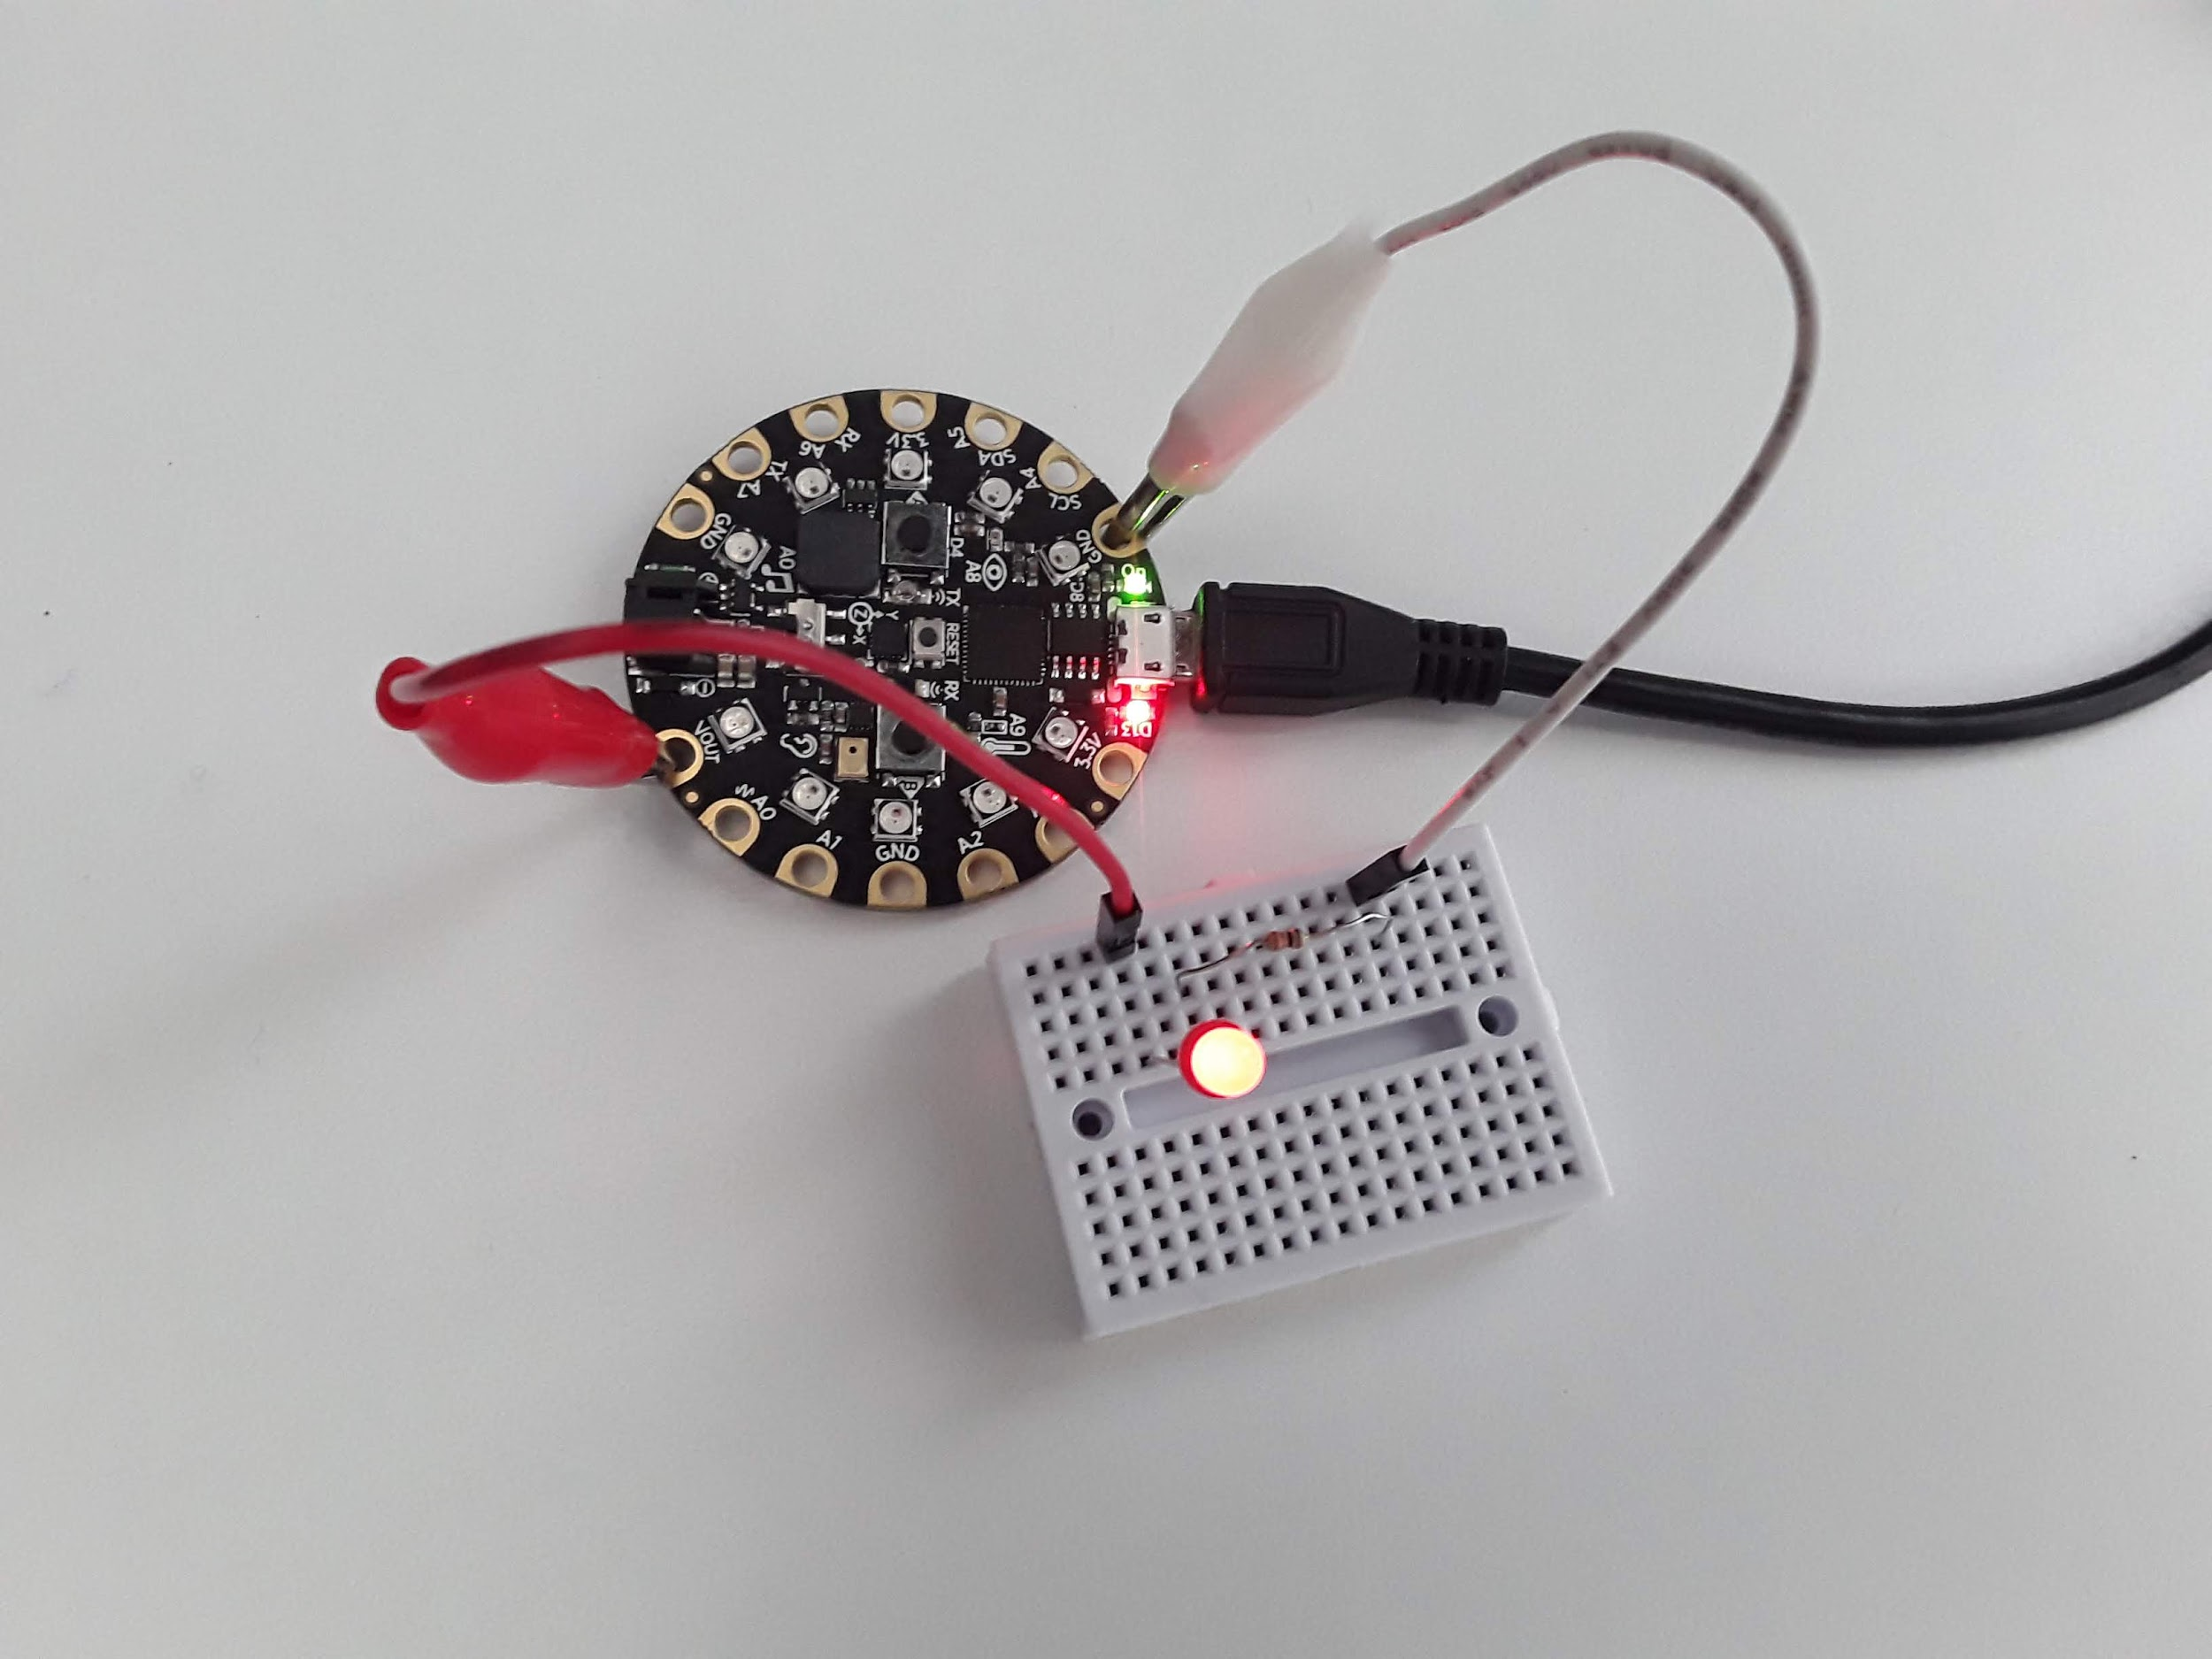
\includegraphics[width=\textwidth]{Figures/LED1.jpeg}
  \end{center}
\end{figure}
Once you have that circuit working, wire up the circuit again with the
3.3V output. Do you notice anything different when you hook up the
circuit with different pins? Here’s my circuit. Do you notice
something different about the intensity of the LED? Why is it
different?
\begin{figure}[H]
  \begin{center}
    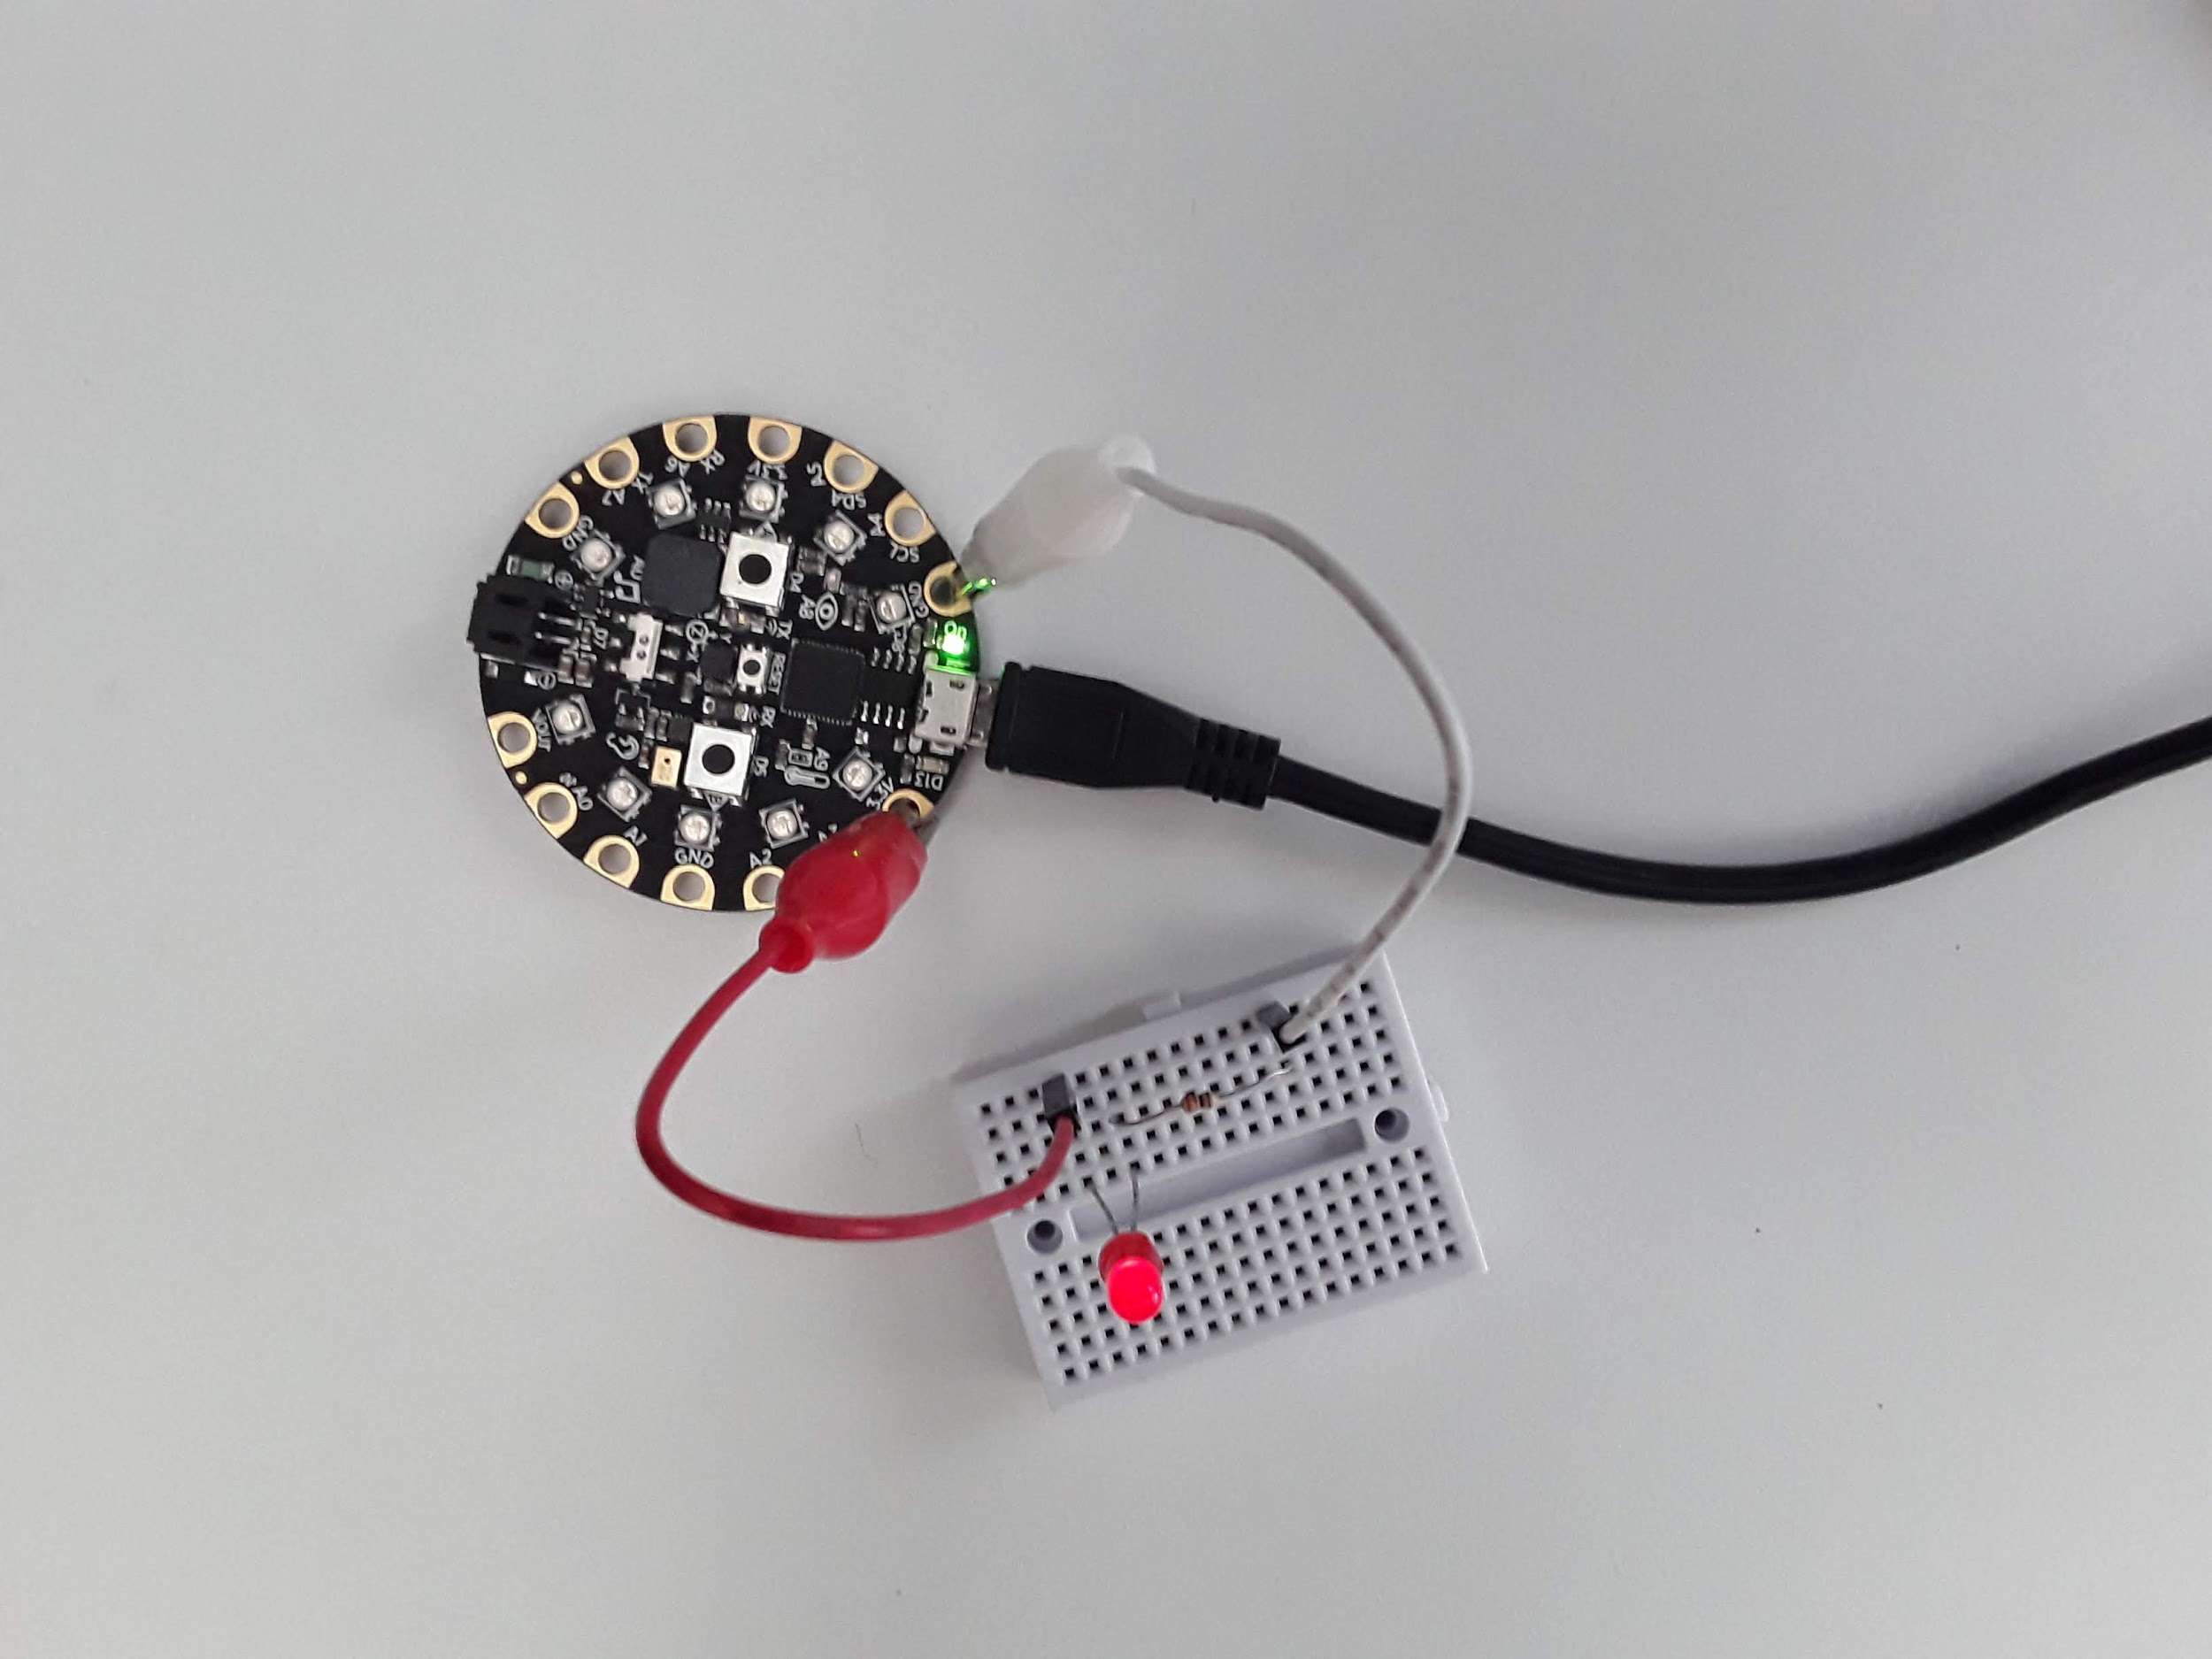
\includegraphics[width=\textwidth]{Figures/LED2.jpeg}
  \end{center}
\end{figure}
\subsection{LED with a push button}

Now that we understand breadboards a bit, we’re now going to manually
blink the LED using a push button placed 
onto the breadboard and have it act like a switch. Therefore, when the
button is pressed, the LED will turn on and when the button is
released the LED will turn off. The button just acts like a wire so
you can plug in the button anywhere in the circuit.
\begin{figure}[H]
  \begin{center}
    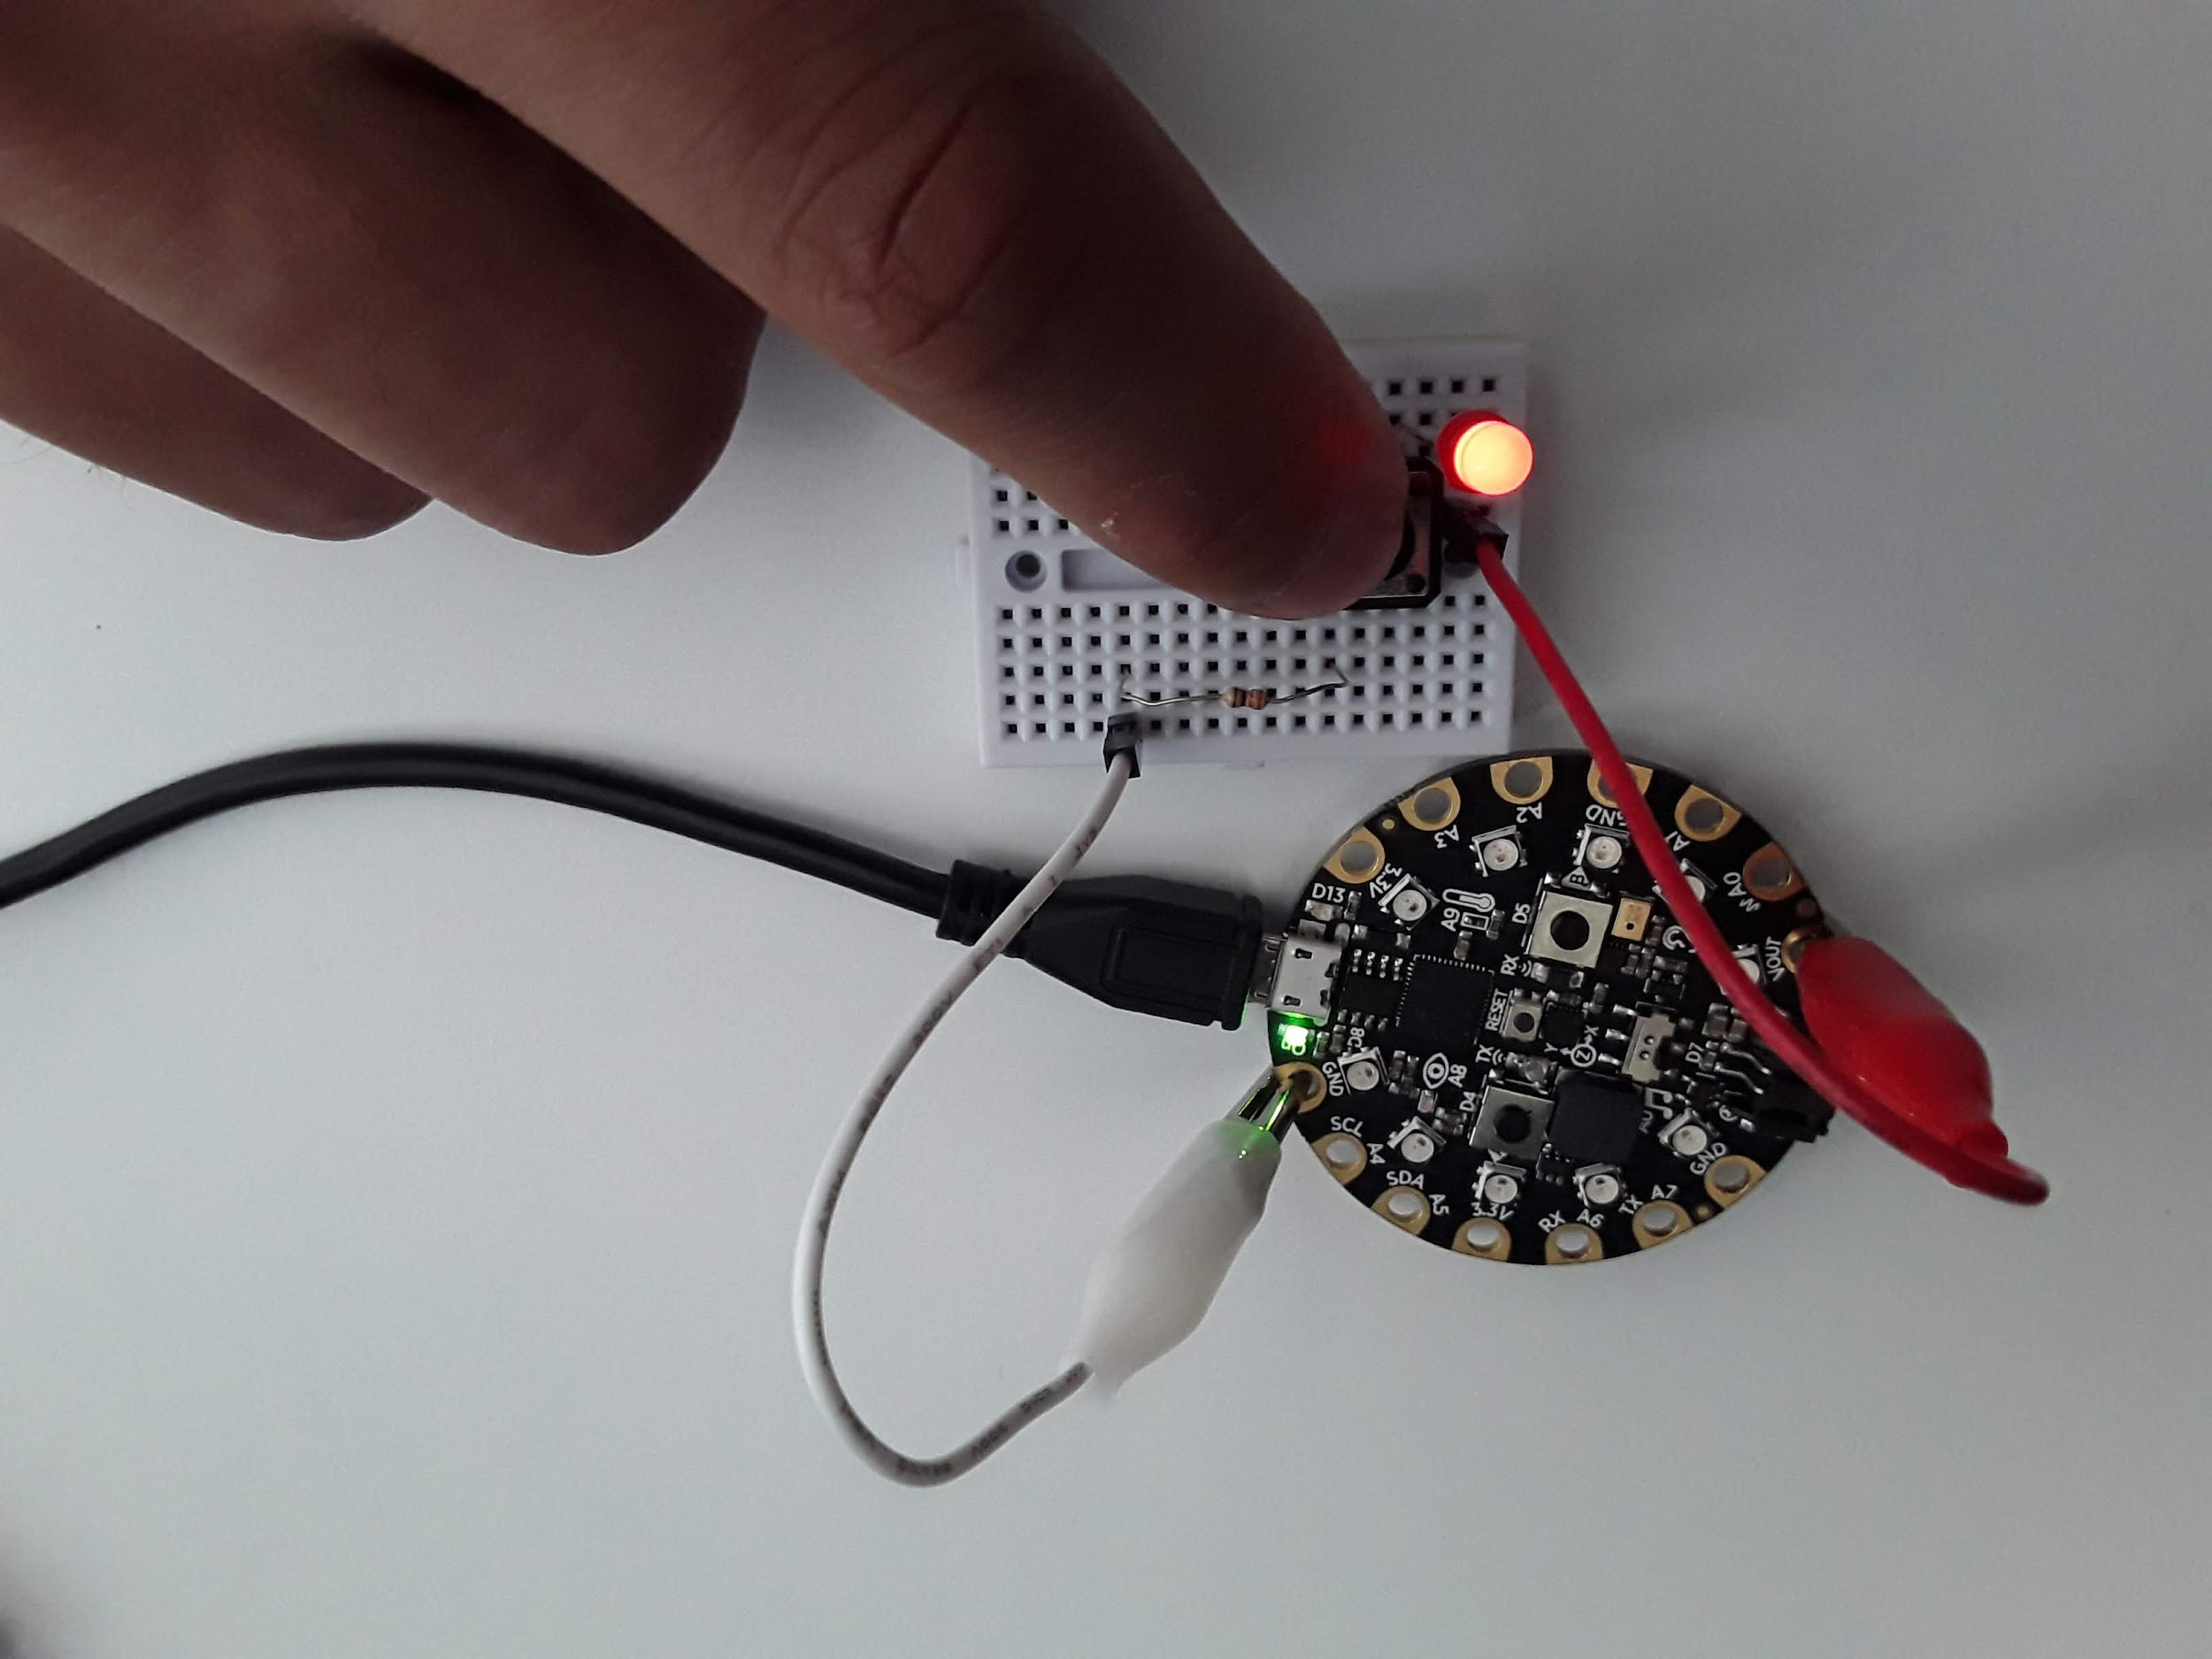
\includegraphics[width=\textwidth]{Figures/LED3.jpeg}
  \end{center}
\end{figure}

\subsection{LED with code}

Next I want you to remove the button from the circuit and wire up the
LED like you had it when the positive end was connected to VOUT or
3.3V. Except this time I want you to hook the positive end of the
circuit to pin A2. Then edit your blink code to blink pin A2. Take
a look at the blink 
code. Right now the code is blinking pin D13. How do you think you
need to change the code to blink pin A2? Here’s what my circuit looks
like for this one. I won’t include code for this one since you just
need to change one line of code.
\begin{figure}[H]
  \begin{center}
    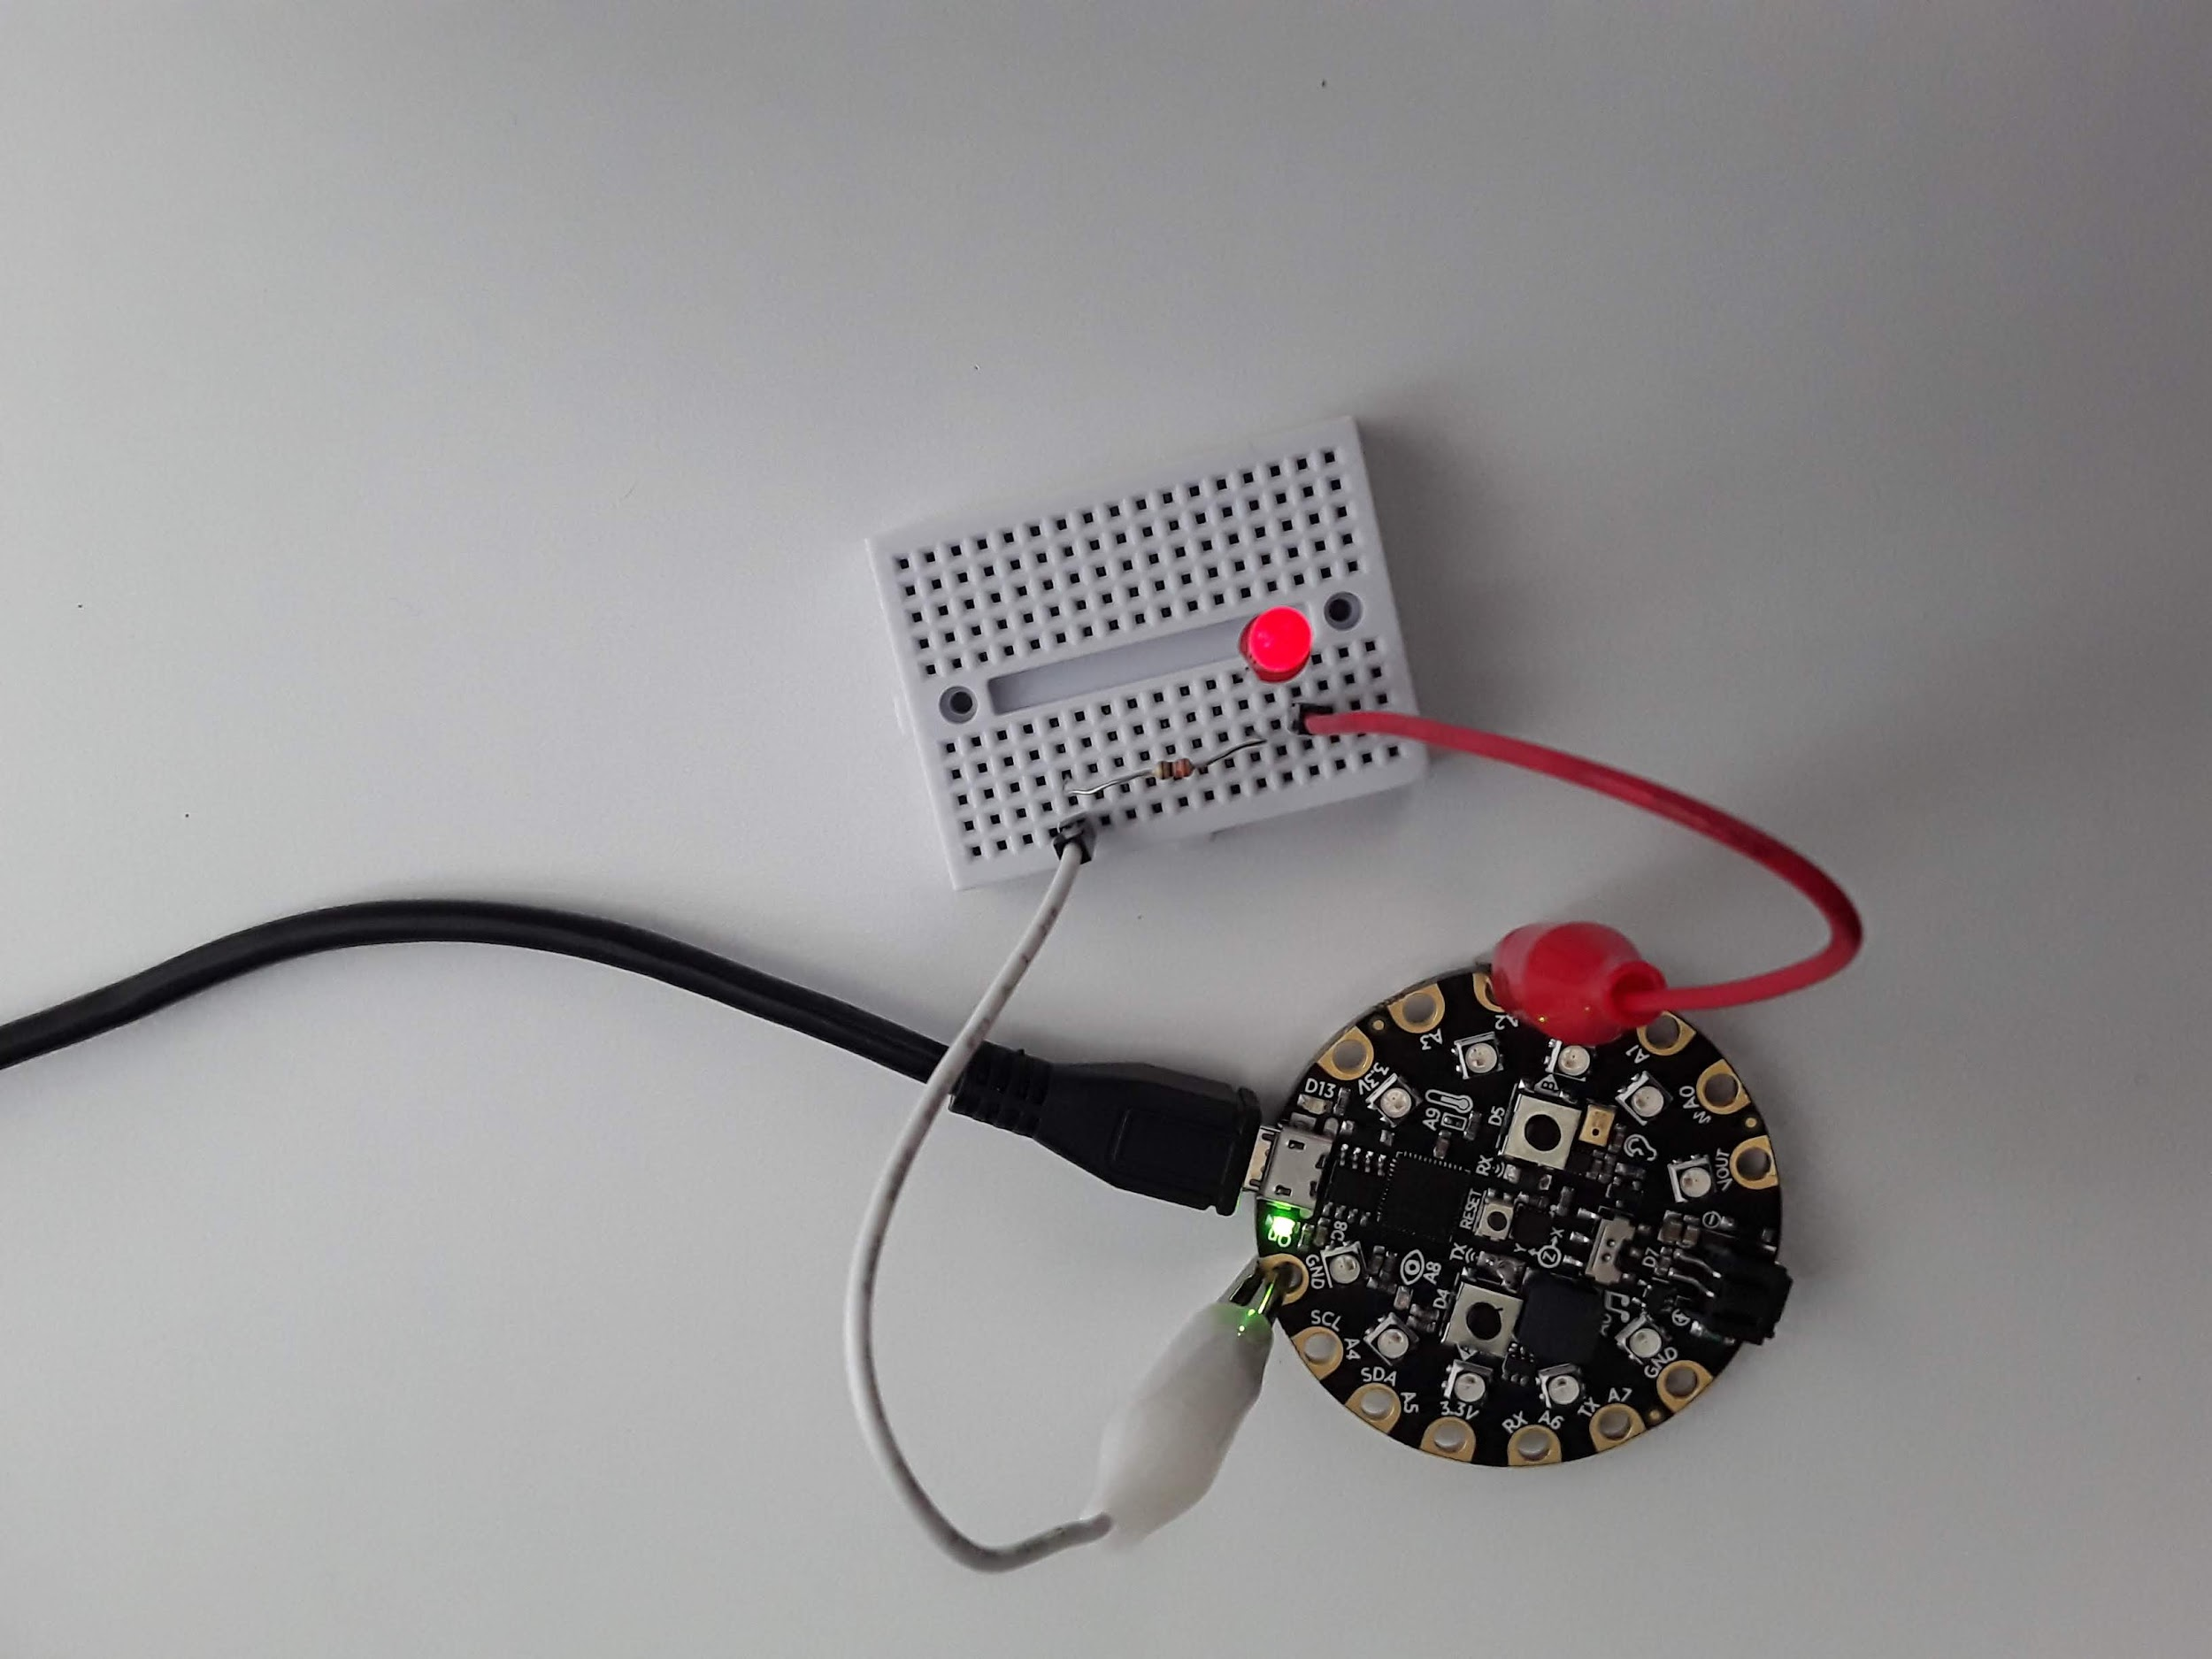
\includegraphics[width=\textwidth]{Figures/LED4.jpeg}
  \end{center}
\end{figure}

\subsection{LED with CPX button}

Finally, I want to use one of the buttons on the CPX to blink the LED
hooked up to pin A2. For this code to work you first need to detect a
button press and then tell the program to change the light from True
to False depending on what it’s current status is. This one is a bit
more difficult so I’ll include the code here and discuss the code
itself. Here is my circuit (identical) to the previous one with Button
A on the CPX pressed down. 
\begin{figure}[H]
  \begin{center}
    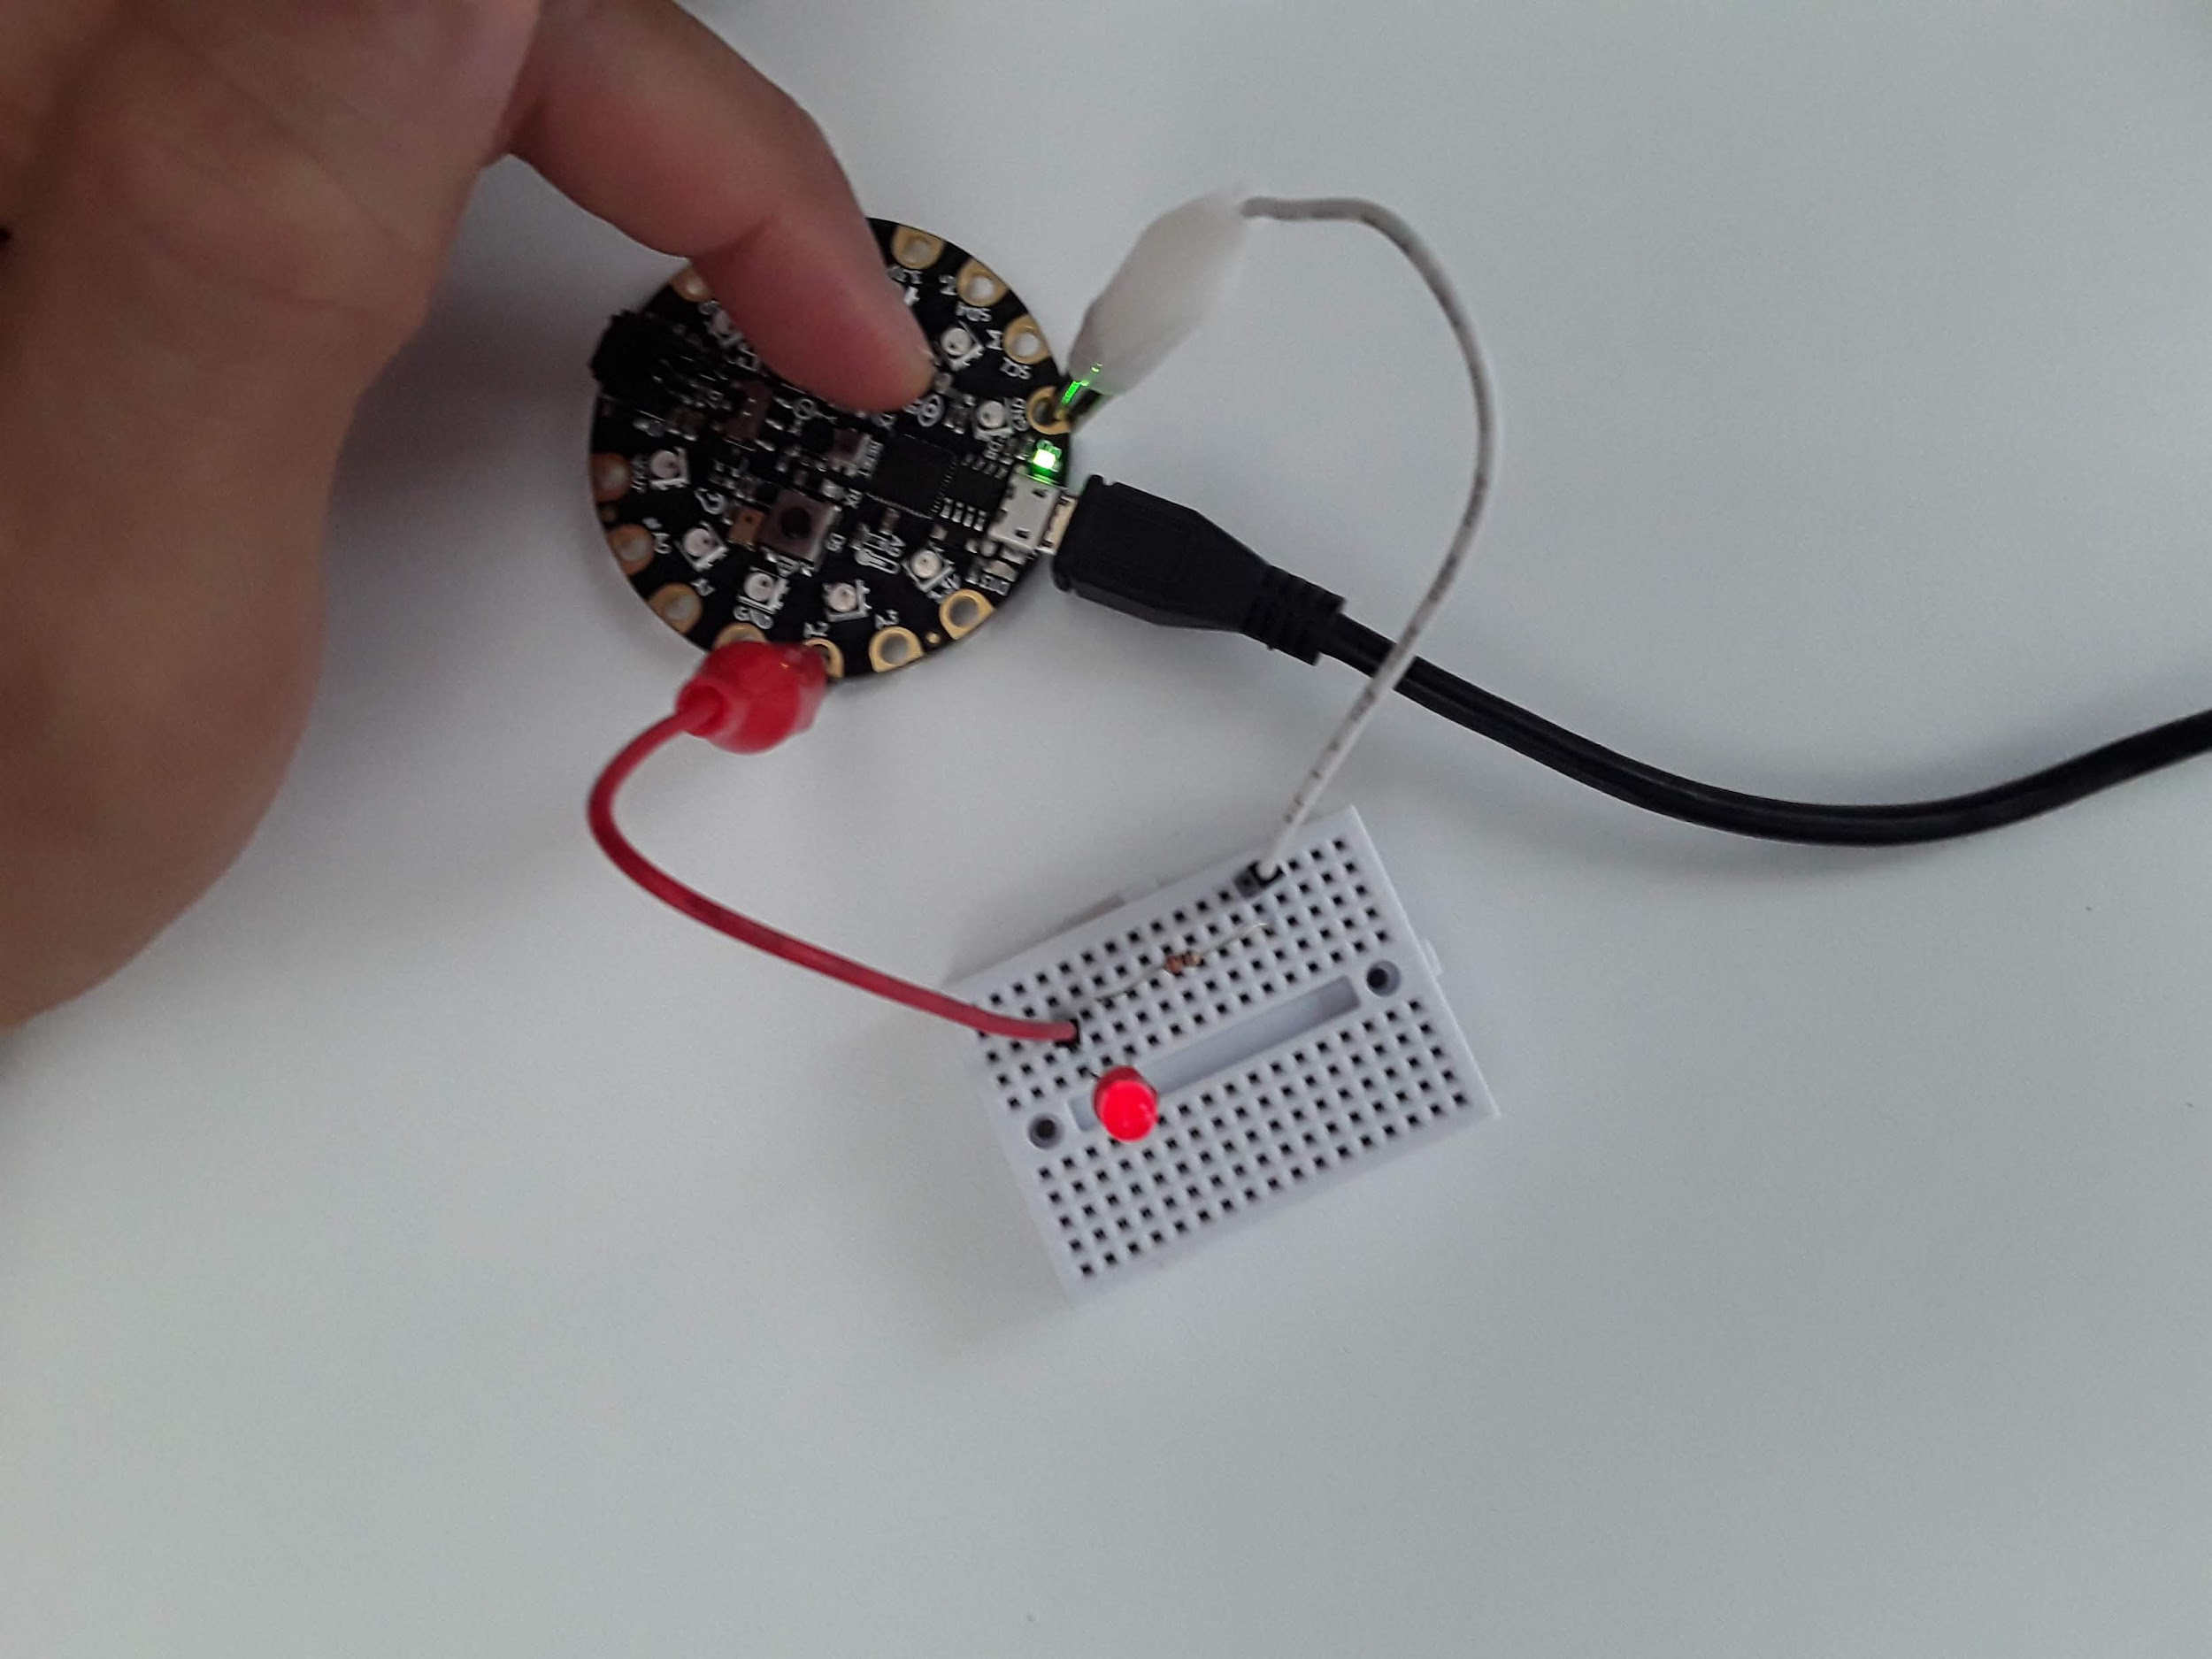
\includegraphics[width=\textwidth]{Figures/LED5.jpeg}
  \end{center}
\end{figure}
Alright so how do we detect a button press? Well the documentation on
this is not so straight forward. What we want to do is detect the
INPUT of a digital signal and then do something if we detect that
signal. Here’s the code I created to get it to work.
\begin{figure}[H]
  \begin{center}
    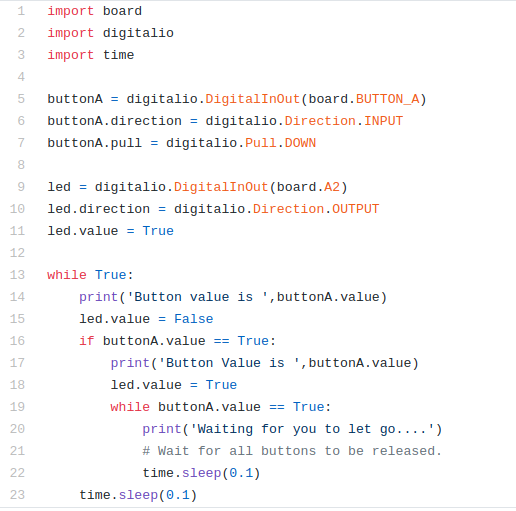
\includegraphics[width=\textwidth]{Figures/button_blink.png}
  \end{center}
\end{figure}
The code above is an image. You could type exactly what you see and
hope you don't type any errors (which is highly unlikely) or you could
look for my code on my
\href{https://github.com/cmontalvo251/Microcontrollers/tree/master/Circuit_Playground/CircuitPython}{Github}. Have
you bookmarked this link yet? I recommend you do so!!! So you're
making a code about Buttons....hmmm. Click that Github link. Where do
you think the code about Buttons is located? Anywho, let's talk about
the code.

The first 3 lines are exactly the same as before. Line 5 through 7 are
similar to creating the “led” variable except we’re using {\it BUTTON\_A} as
the board value and setting the direction to {\it INPUT}. Finally we’re
setting the pull direction to {\it DOWN}. This means the button acts like a
pull down resistor and when it’s pressed the value of the button goes
{\it HIGH}.

Lines 9-11 are the same as before. We create an led variable and tell
the CPX that the led is hooked up to pin A2. We then start the while
loop on line 13. First if you click the Serial button you’ll see the
text ‘Button value is False’. It’s False because {\it buttonA.value} is not
being pressed. On line 15 the led is set to False (turned off). On
line 16 the button value is checked using an if statement as to
whether or not the button is pressed (True). If the button is pressed,
the user will be notified that the button is pressed on line 17 and
the led will be set to True (on) in line 18. Lines 19-22 are while
loop that will notify the Serial monitor that you must let go of the
button before the code can continue to the main while loop. The
{\it time.sleep} functions are there to make sure a human can operate the
button without code running faster than a human can press a
button. When I press the button down here is the output I get from the
{\it Serial} monitor. 
\begin{figure}[H]
  \begin{center}
    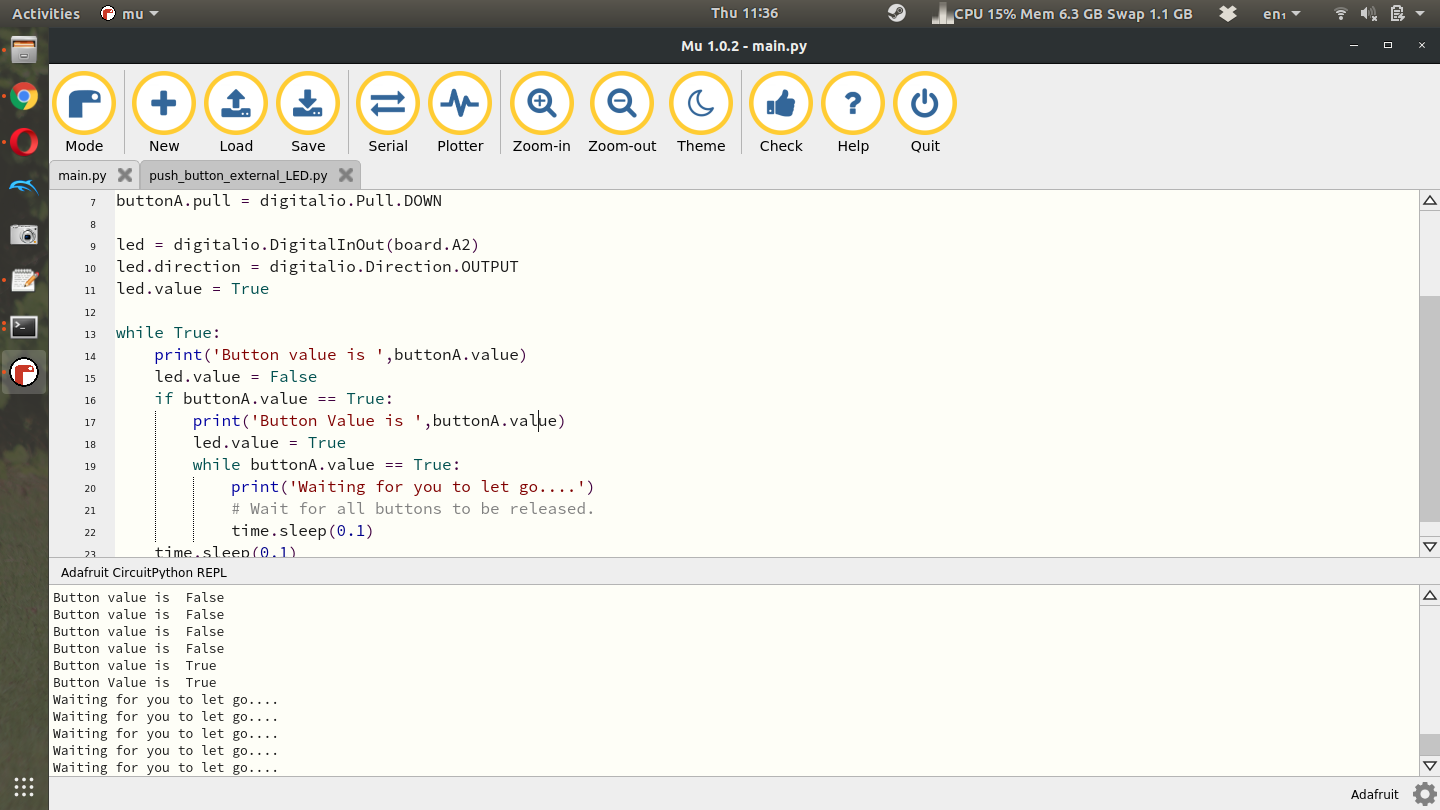
\includegraphics[width=\textwidth]{Figures/MuButton.png}
  \end{center}
\end{figure}
Here you’ll see 4 lines that say ``Button value is False" and then two
lines that say ``Button value is True" followed by 5 lines that say
``Waiting for you to let go...". See if you can get this code to work and
play with it and modify it as you see fit. By the way, the LED
connected to pin D13 has this exact same circuitry, an LED a resistor,
it’s all just soldered to the PCB so you don’t have to build it using
a breadboard. Hopefully now you have some appreciation for buttons and
LEDs!! 

\subsection{Assignment}

Once you've completed the project above, upload a PDF with all of the photos and text
below included. My recommendation is for you to create a Word document
and insert all the photos and text into the document. Then export the
Word document to a PDF. For videos I suggest uploading the videos to
Google Drive, turn on link sharing and include a link in your
PDF. Note that all code must be included in the appendix or you'll be
penalized 10\%. 


\begin{enumerate}[itemsep=-5pt]
\item Include a photo of your circuit with your LED turned on using VOUT (make sure your face is in the photo) - 20\%
\item Include a photo of your circuit with your LED turned on using 3.3V (make sure your face is in the photo) - 20\%
\item Include a video of you turning your LED on and off with the push button (again make sure your face is in the video for enough time to say who you are and say hello) - 20\%
\item Include a video of your LED blinking on and off automatically by modifying the blink code (make sure your face is in the video for enough time to say who you are and say hello) - 20\%
\item Include a video of your LED blinking by pressing a button on the CPX. Note the LED must blink while you press and hold the button. You'll need to modify the code to get that to work. (make sure your face is in the video for enough time to say who you are and say hello) - 20\%
\end{enumerate}


\section{Using the CPX/CPB as a Data Acquisition System (DAQ)}
\label{s:daq}

\subsection{Parts List}

\begin{enumerate}[itemsep=-5pt]
\item Laptop
\item CPX/CPB
\item USB Cable
\end{enumerate}

\subsection{Learning Objectives}
\begin{enumerate}[itemsep=-5pt]
\item Record real time measurements from the CircuitPlayground using the Serial monitor
\item Learn how to use the typing module to type data directly into a spreadsheet or text file
\item Learn how to log data on the on board memory of the CircuitPlayground 
\end{enumerate}

\subsection{Extra Help}

This is a pretty hard project to do with multiple different
methods. After you’ve read through this document I suggest you watch
a youtube I created on \href{https://youtu.be/yX0zeIfn2j4}{Logging Data with the Circuit Playground
Express}. I have also made video where I \href{https://www.youtube.com/watch?v=Vc7_KxRnORI}{log temperature and
accelerometer data using on board memory with the CircuitPlayground
Bluefruit.}

\subsection{Getting Started}

Taking data is the core of any instrumentation project. Data
Acquisition Systems or DAQ for short come in all shapes and
sizes. Believe it or not the CPX can be used as a crude and cheap
DAQ. The CPX can easily take temperature data and monitor the
temperature in a greenhouse or take humidity readings of a plant to
monitor soil content. Before we learn about the different sensors on
board the CPX, we want to make sure we can store that data later
rather than just having it spit data out via the serial monitor. For
starters though let’s get the CPX to print out something simple like
button presses since we’ve touched on that already. The code I’m using
is shown below and can also be found on
\href{https://github.com/cmontalvo251/Microcontrollers/blob/master/Circuit_Playground/CircuitPython/Data_Logging/button_presses.py}{Github}.
\begin{figure}[H]
  \begin{center}
    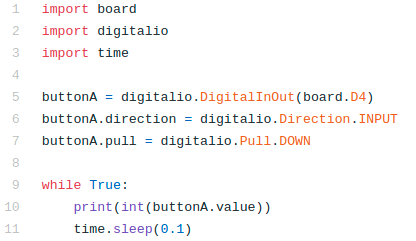
\includegraphics[width=\textwidth]{Figures/button_presses.png}
  \end{center}
\end{figure}
The code is pretty similar to what I had in the past. I import board,
digitalio, and time. I create a buttonA object using the digitalio
library to record button presses. I then enter into a while loop print
the buttonA.value. The difference here is that I use the int()
function to convert the buttonA.value to an integer. The reason why I
do this is because buttonA.value is a boolean. It is either True or
False. An integer though is a number and thus a value of False is 0
and True is 1. If you open the serial monitor and push the A button
down a few times you’ll see some zeros and 1’s.
\begin{figure}[H]
  \begin{center}
    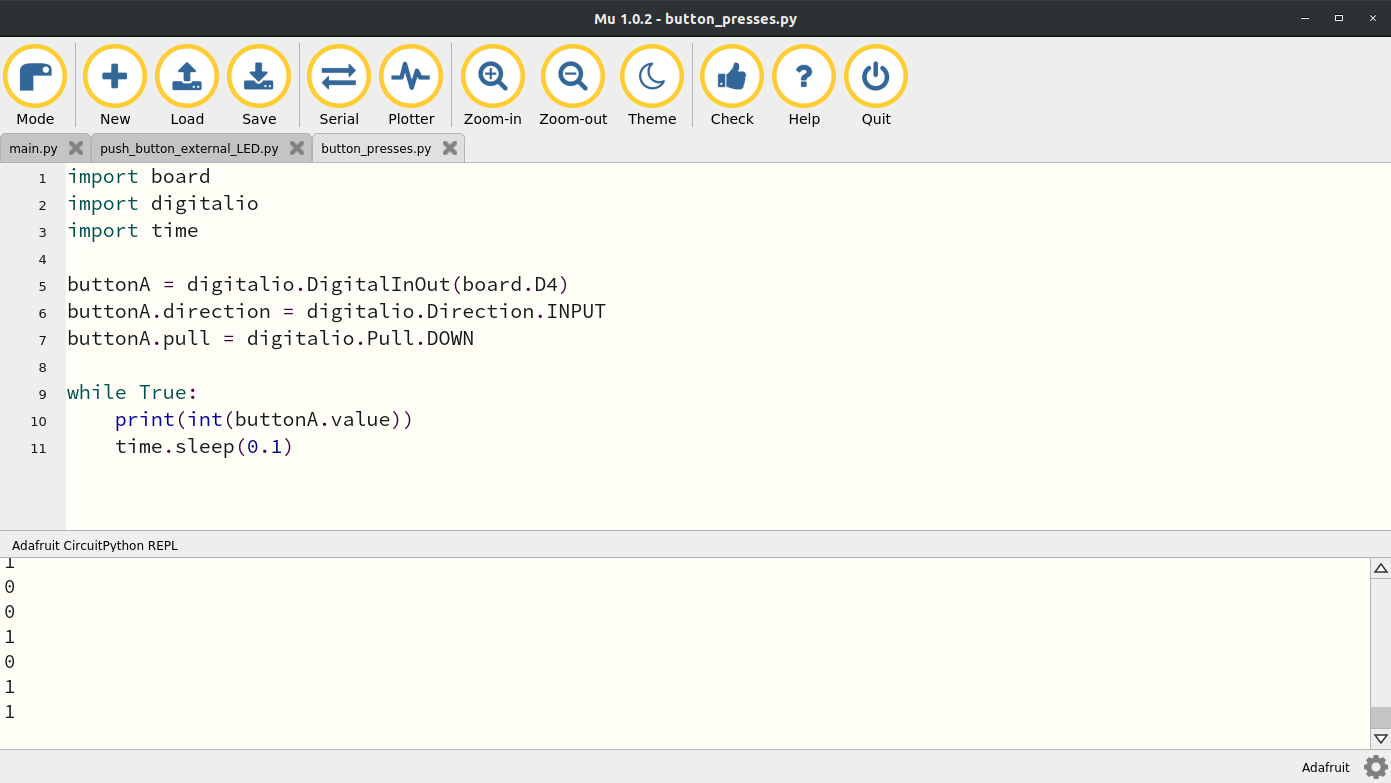
\includegraphics[width=\textwidth]{Figures/MuButtonPress.png}
  \end{center}
\end{figure}
Mu also has a really neat builtin plotter. You’ll see next to the
Serial button there is a button called Plotter. If you click that
button now nothing will pop up on the screen. Unfortunately in order
to plot using the Plotter you need to modify the print() statement to
this:
\begin{verbatim}
print((int(buttonA.value),))
\end{verbatim}
Notice the extra parentheses and the comma. Now if you click Plotter
you’ll see something like this. You’ll notice that the print statement
now has commas in it and the Plotter is recording button presses. 
\begin{figure}[H]
  \begin{center}
    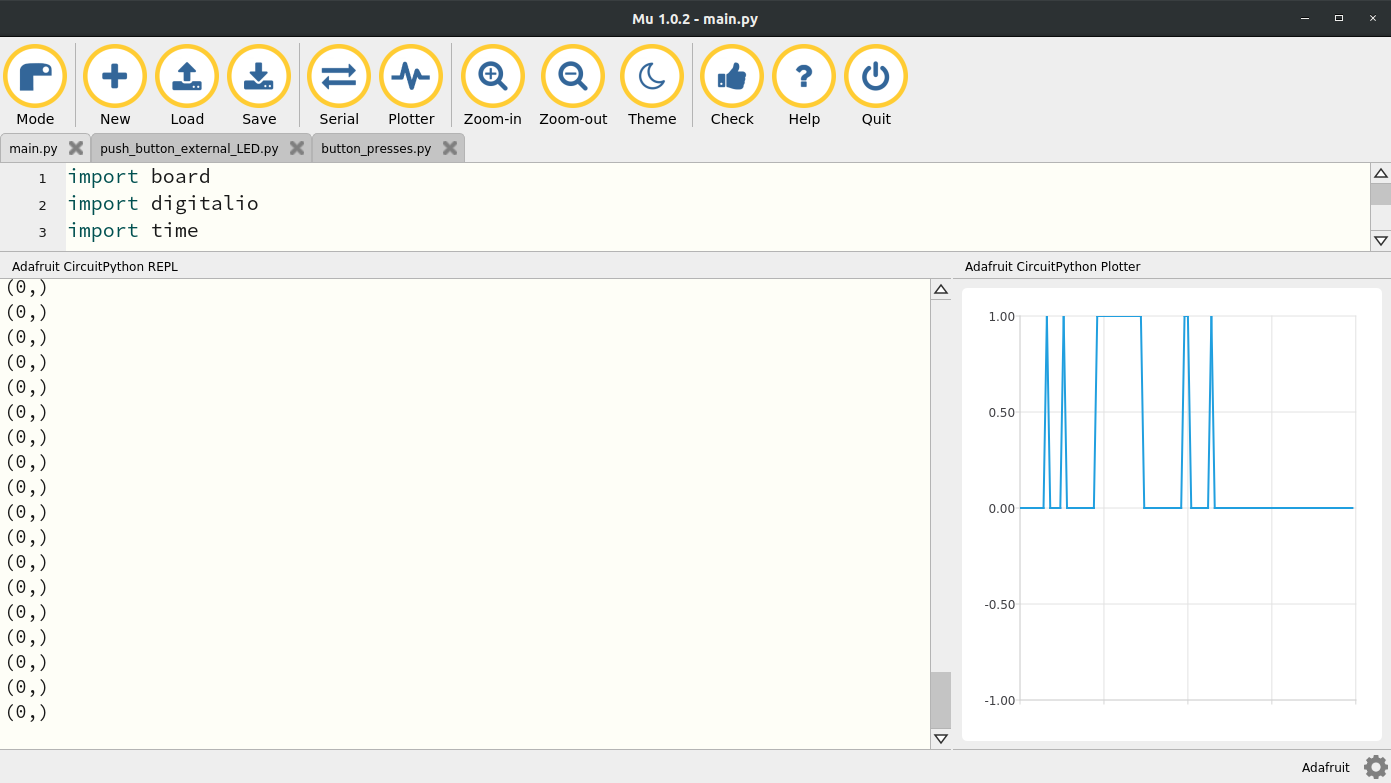
\includegraphics[width=\textwidth]{Figures/MuPlotter.png}
  \end{center}
\end{figure}
The problem with this is we still can’t save the recorded data
anywhere. Before we get into saving data let’s first edit the print
statement again to get rid of the Plotter by removing the extra
parentheses and add time.monotonic() that way we can keep track of
when a button was pressed. My print statement looks like this now: 
\begin{verbatim}
print(time.monotonic(),int(buttonA.value))
\end{verbatim}
Looking at the serial monitor now you’ll see that time is being
printed alongside the button presses. 
\begin{figure}[H]
  \begin{center}
    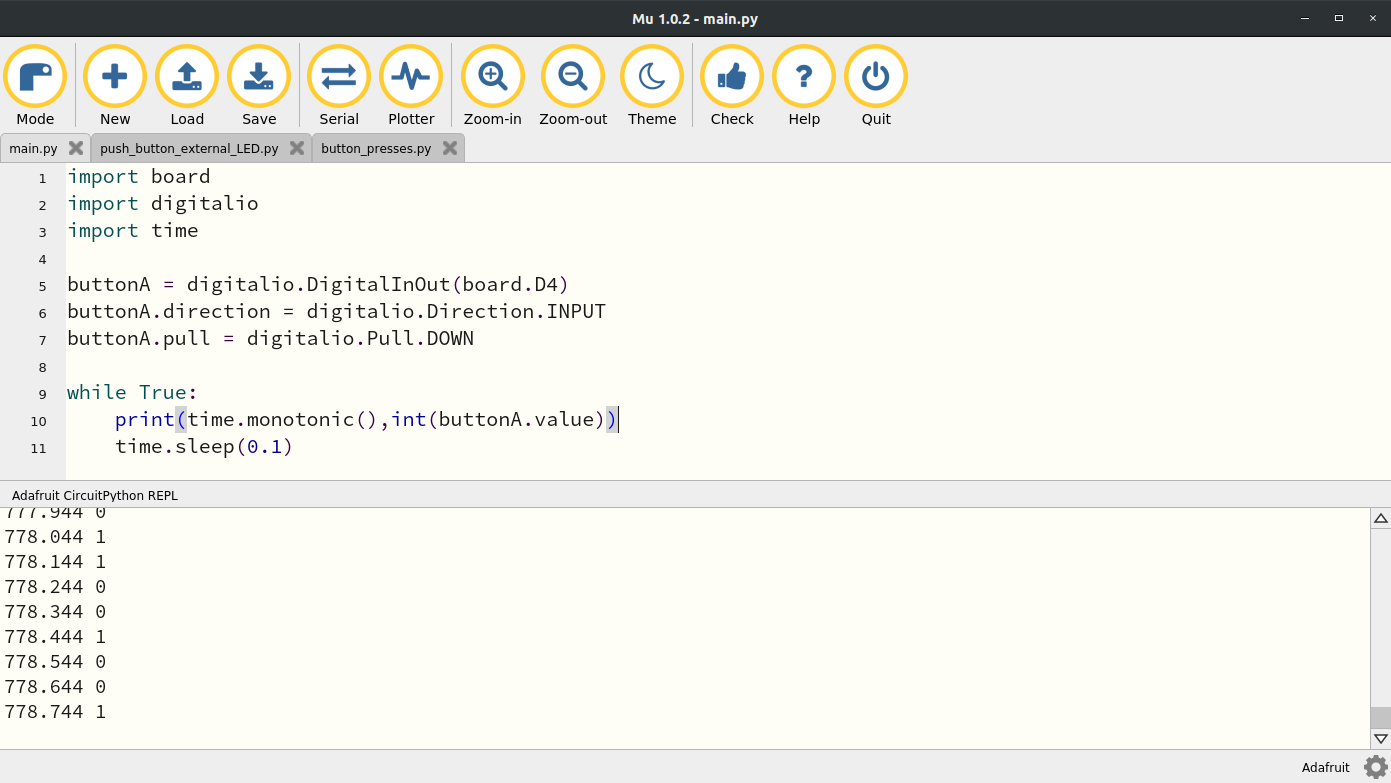
\includegraphics[width=\textwidth]{Figures/MuPlotterTime.png}
  \end{center}
\end{figure}
Now we are in a position where we can record some data and save it to
our computer. There are 3 ways to record data. I call the first,
Method1 and you basically just copy and paste from the serial monitor,
Method2 where you have the CPX/CPB type data into a spreadsheet and
Method3 where you log data internally onto the CPX/CPB itself.

\subsection{Method 1 - Copying Serial Monitor Data}

If you open up the serial monitor you can see the data output. If you
unplug the CPX while it’s taking data the code will stop. {\bf Note: In
newer versions, unplugging your CPX will result in a loss of data. If
this happens try pressing CTRL+C after you click the REPL window.} With
the code stopped you can select all the data in the Serial monitor and
then copy and paste the data into a text file on your computer. You
can actually copy this into a new file on Thonny and just save it as a
*.txt file. Once you have the data in a text file you can proceed to
plotting in Python on your desktop which I discuss in the last
section.Here’s some example data in Gedit which is a simple text
editing program.
\begin{figure}[H]
  \begin{center}
    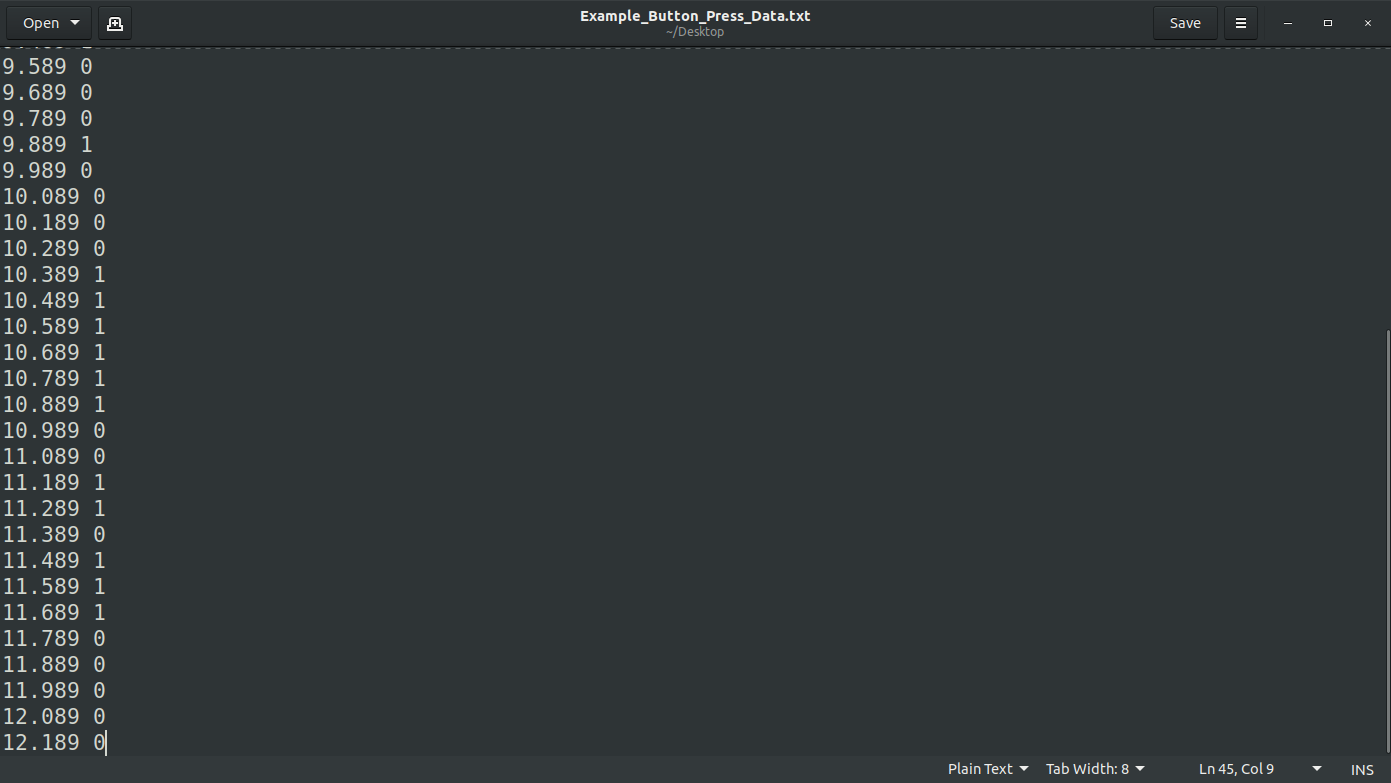
\includegraphics[width=\textwidth]{Figures/Gedit_Data.png}
  \end{center}
\end{figure}

\subsection{Method 2 - Automatically Populate a Spreadsheet}

The downside with the above method of course is if you have a ton of
data to record you could lose the data or run into a massive copy and
paste issue. The second option is to use this module called keyboard
which takes control of your keyboard on your desktop computer and
actively types your data into a spreadsheet. The code is very
extensive but I’ll include the simple one here so we can discuss
it. Below are the first 30 lines of code. The first 6 lines of code
are just comments since I heavily adopted this code from the \href{https://learn.adafruit.com/make-it-a-keyboard/circuitpython}{Adafruit
Learn System}. \href{https://github.com/cmontalvo251/Microcontrollers/blob/master/Circuit_Playground/CircuitPython/Data_Logging/record_button_presses_typing.py}{My version of this code} can be found on my Github. Lines 8 -
14 are import commands as we’ve seen previously. The regular import
modules board, time and digitalio are imported but we are also
importing the Keyboard module so that the CPX can takeover our
keyboard. Lines 16-22 create two buttons. First we create buttonA
attached to pin D4 and then a switch attached to pin D7. If you look
on the CPX there is a switch labeled D7. Before you copy this code
onto the CPX make sure you move the switch towards the ear looking
symbol. Lines 26-28 created the keyboard object. We are going to call
it layout for this example code.
\begin{figure}[H]
  \begin{center}
    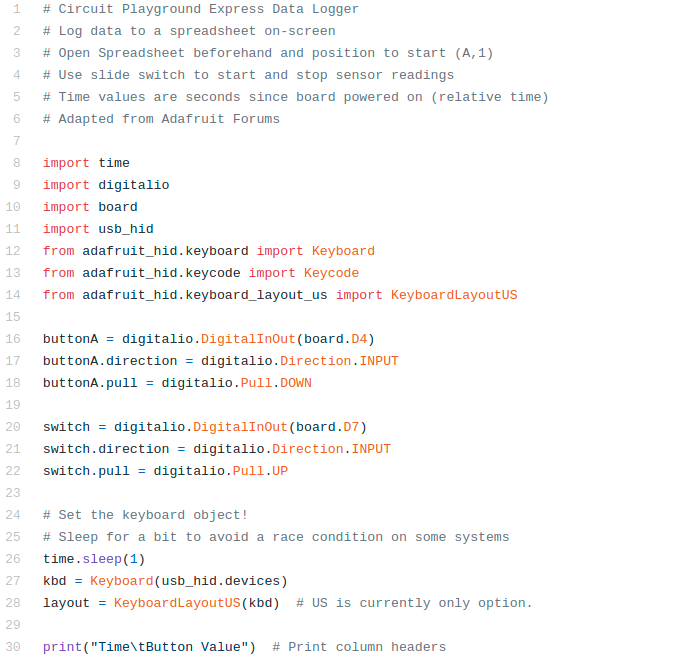
\includegraphics[width=\textwidth]{Figures/Typing1.png}
  \end{center}
\end{figure}
The next 30 lines are shown below. Lines 32-35 define a
function. Functions in Python have a pretty standard structure. The
keyword def is used to denote that the next line is a definition for a
function. The name of the function is {\it slow\_write()}. The input to the
function is string which ironically enough is a string object. Line
33-35 define what the function does. Line 33 sets up a for loop where
the code loops through each character in the string. Everytime it gets
to a new character it will use your keyboard to type that character
using the layout.write(c) command. The time.sleep(0.02) is just to
slow down the keyboard so your computer can keep up. That function is
defined above the standard while True: statement on line 37 but is
called on line 42. You’ll see there is a {\it slow\_write(output)} on line
42. In this case output is a string and it’s sent to the function
{\it slow\_write()}. So in this case we have a function that can write a
string so we just need to take data and then write it using our
keyboard. Line 38 is an if statement that will only be true if the
switch on pin D7 is pushed towards the music note on the CPX. If the
switch is not thrown the code will move to the else statement on line
52 and tell the user that you need to flip the switch. If the switch
is thrown line 40 will take data for us. First it will record the
time.monotonic() and store it as a floating point number using the
\%0.1f designation which means that it will store 1 decimal as a
\%floating point number for f.
\begin{figure}[H]
  \begin{center}
    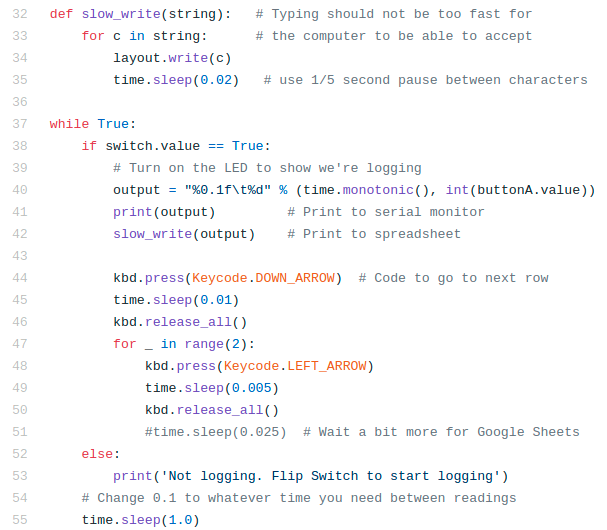
\includegraphics[width=\textwidth]{Figures/Typing2.png}
  \end{center}
\end{figure}
The second number in the string is an integer or a base 10 (decimal)
integer designated by the \%d part of the format. The integer is
int(buttonA.value). You’ll see a \t in between the formatted numbers
which is a tab. The tab is there to tab between cells in a
spreadsheet. Line 41 will print the output string to the Serial
monitor and it will also type the contents of the string. Very
important here. When you flip the switch on the CPX your keyboard will
start typing in whatever active window is selected. If you don’t have
a spreadsheet opened and active (selected), the keyboard will just
begin typing in whatever window is open. Make sure you have a
spreadsheet program open and ready to go. Lines 44-51 tell the
keyboard to hit the {\it DOWN\_ARROW} on your keyboard to move to the next
row and the {\it LEFT\_ARROW} twice to move back to the first column. Line 55
is a sleep to only log data once a second. I ran this code for a bit
and had it type into LibreOffice Calc which is a free spreadsheet
program. Google Sheets or Microsoft Excel will also work just fine. 
\begin{figure}[H]
  \begin{center}
    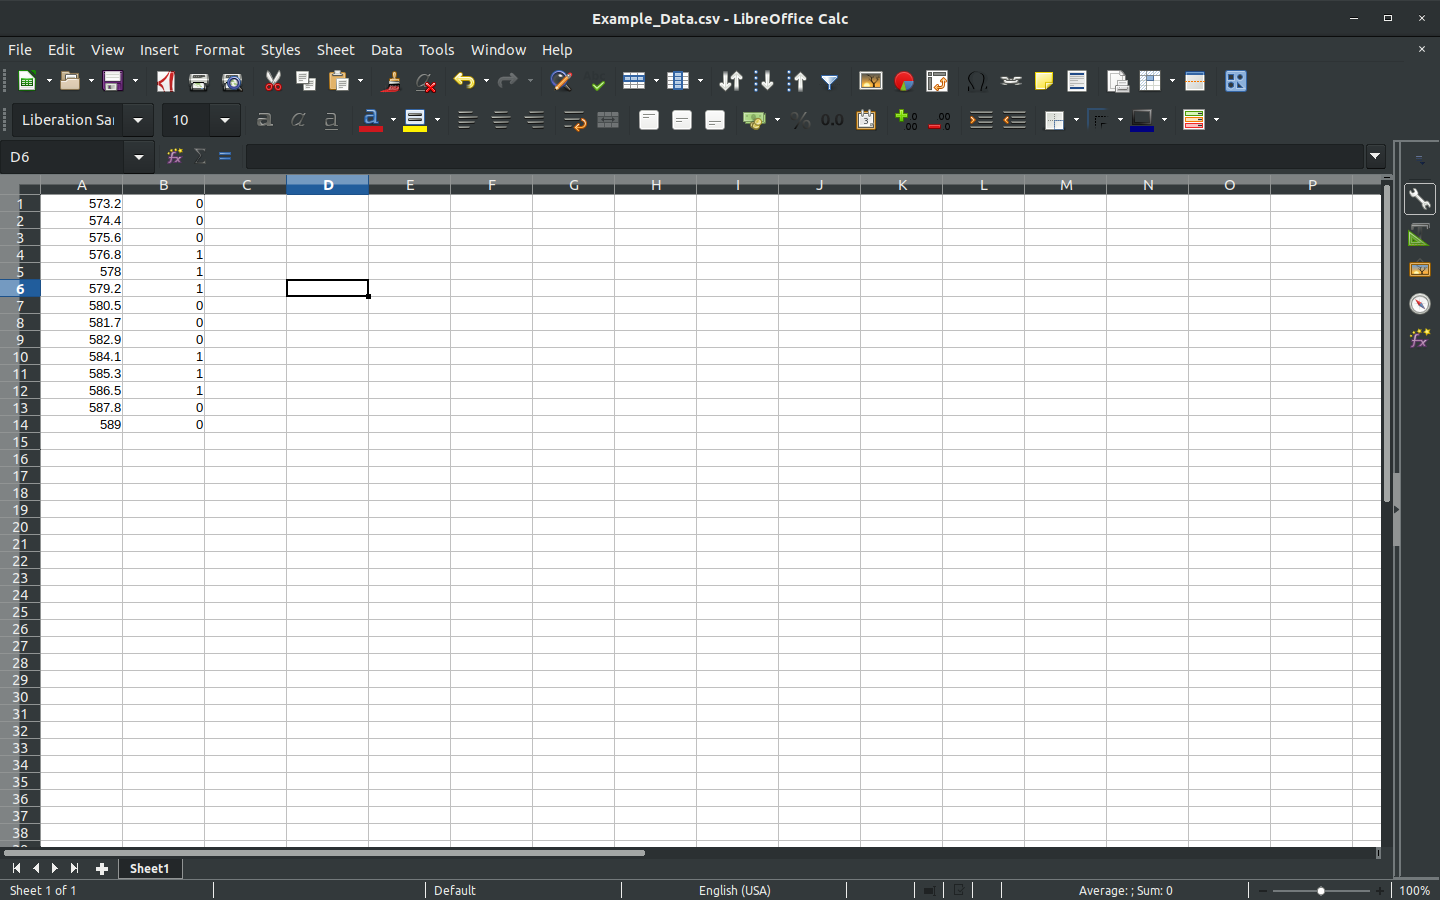
\includegraphics[width=\textwidth]{Figures/Typing3.png}
  \end{center}
\end{figure}
You’ll see that the first column is time with 1 decimal point and the
second column is the button press values. At this point you must click
{\it Save As...} and save the document as a CSV which stands for Comma
Separated Value. Once you have the file saved you can proceed to
plotting in Python on your Desktop. 

\subsection{Method 3 - Logging Data Directly to on board memory}

The problem with the above 2 methods is that you need a laptop to log
data in the field. It would be nice if you could use the optional
battery pack and just have the CPX log data on the CPX itself. This is
the most complex way but in my opinion the best way. In order to get
this to work you need to allow the drive on the CPX to have read/write
permissions. This requires you to load a piece of software called
boot.py and put it on the CPX. I have this
\href{https://github.com/cmontalvo251/Microcontrollers/blob/master/Circuit_Playground/CircuitPython/Data_Logging/boot.py}{software
  on my Github}. The software is shown below. The first 10 lines are
probably very familiar. Import some modules and then create a switch object. Line 13
is where all of the storage permissions are changed. If the flip is
switched towards the A button, the storage module is used to allow you
to write to the CPX. The problem here is that if you do this, you
won’t be able to edit code. I’ll explain the procedure here in a
minute. As always, the relevant Adafruit tutorial is on the \href{https://learn.adafruit.com/adafruit-circuit-playground-express/circuitpython-storage}{Adafruit
Learn System} if you want to read more about it. Again make sure you
store this file onto the CIRCUITPY drive and save it as boot.py
\begin{figure}[H]
  \begin{center}
    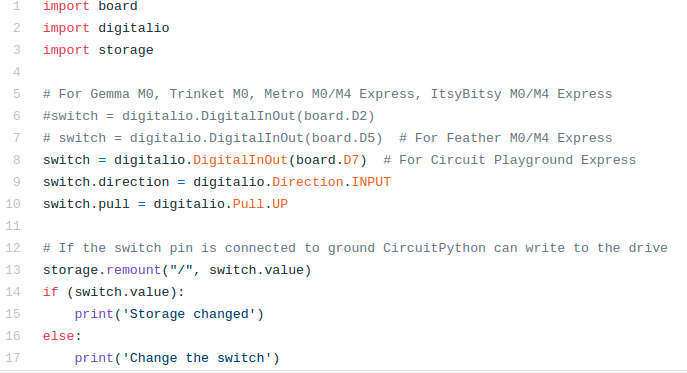
\includegraphics[width=\textwidth]{Figures/boot.png}
  \end{center}
\end{figure}
In addition to storing the file boot.py you’ll need to edit your
main.py script to only log data when the switch is moved towards the B
button. The software to record button presses on disk is shown below
and as always
\href{https://github.com/cmontalvo251/Microcontrollers/blob/master/Circuit_Playground/CircuitPython/Data_Logging/write_button_presses_disk.py}{on
  my Github}. In this software we again see the standard 
commands. Lines 1-3 import all the modules we need and then 5-15
create a switch, a button and an LED. In this case we’re using the LED
soldered to the board. Line 17-20 check to see if the user has flipped
the switch. If the switch is False the storage module on boot.py will
allow the drive to act like a data logger and it will open a file
called {\it Test\_Data.txt} for writing (‘w’). If the switch is True then the
user will be notified that the file has not been opened for
writing. Lines 22 through 33 include the infinite while loop. Line 23
turns the LED on and line 24 prints out the current time and the
button value in integer form. If the switch value is False the program
will create an output string by converting all numbers to strings
using the str function. Notice that there is a {\it
  str(``\textbackslash n")} at the end of
the output variable which tells the computer to write a new line of
data to the file. Lines 28 and 29 write the output to the file from
line 18 and then flush the output which means the CPX waits for the
data to be fully written before moving on. It also turns the LED off
so we know the CPX took data even when we aren’t looking at the Serial
monitor. If the switch value is true it means that the we never opened
the data file and thus we tell the user we aren’t logging data and
it’s time to flip the switch and hit reset. 
\begin{figure}[H]
  \begin{center}
    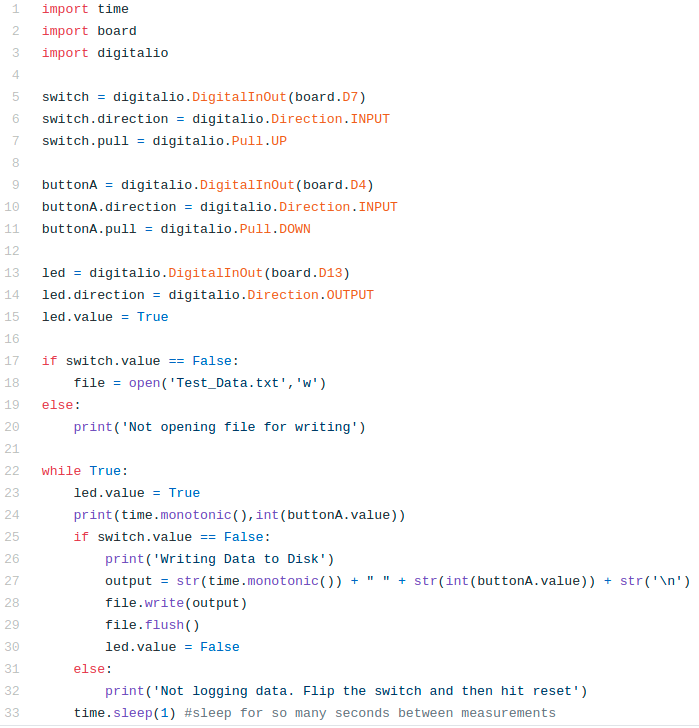
\includegraphics[width=\textwidth]{Figures/method3_1.png}
  \end{center}
\end{figure}
So here is the flow of what you want to do for method 3.
\begin{enumerate}[itemsep=-5pt]
\item Unplug the CPX
\item Flip the switch towards the A button.
\item Plug in the CPX and save the boot.py and main.py files. Remember you can only save Python scripts when the switch is flipped towards the A button.
\item When you are ready to start recording data, flip the switch towards the B button. If you’re looking at the Serial monitor, the software will throw an error. Just ignore it and hit the reset button. When your computer recognizes the CPX you can turn the Serial monitor on and off.
\item When you are done taking data simply slide the switch over towards the A button and hit reset again. This is what my Serial monitor looks like when I do this. You’ll see that I was writing to disk for like 25 seconds and then I flipped the switch back towards the A button.
\end{enumerate}
\begin{figure}[H]
  \begin{center}
    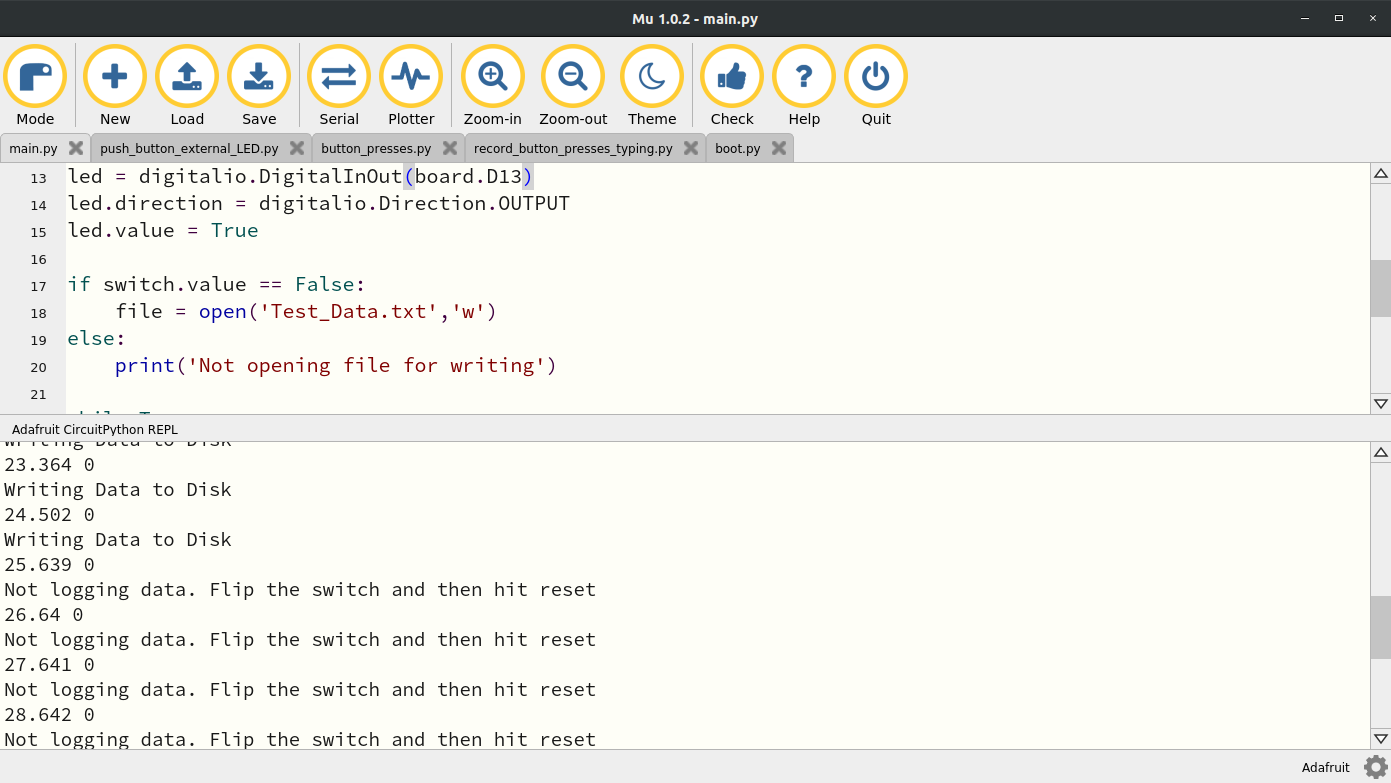
\includegraphics[width=\textwidth]{Figures/method3_2.png}
  \end{center}
\end{figure}
With the switch flipped and data taken, open your folder manager and
take a look at the CIRCUITPY drive. This is what mine looks
like. You’ll see I have two Python files and a file {\it Test\_Data.txt} with
all my data in it. 
\begin{figure}[H]
  \begin{center}
    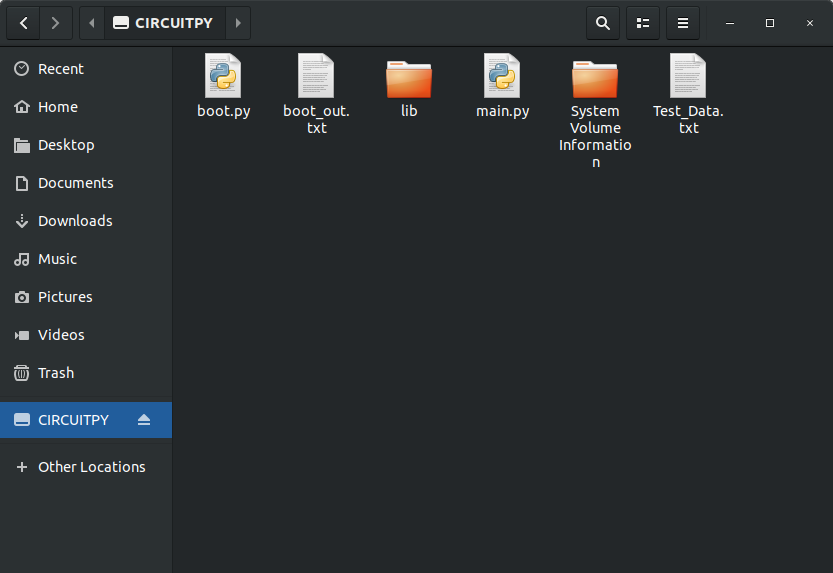
\includegraphics[width=\textwidth]{Figures/method3_3.png}
  \end{center}
\end{figure}
If you open the {\it Test\_Data.txt} file you will hopefully see data in it.
\begin{figure}[H]
  \begin{center}
    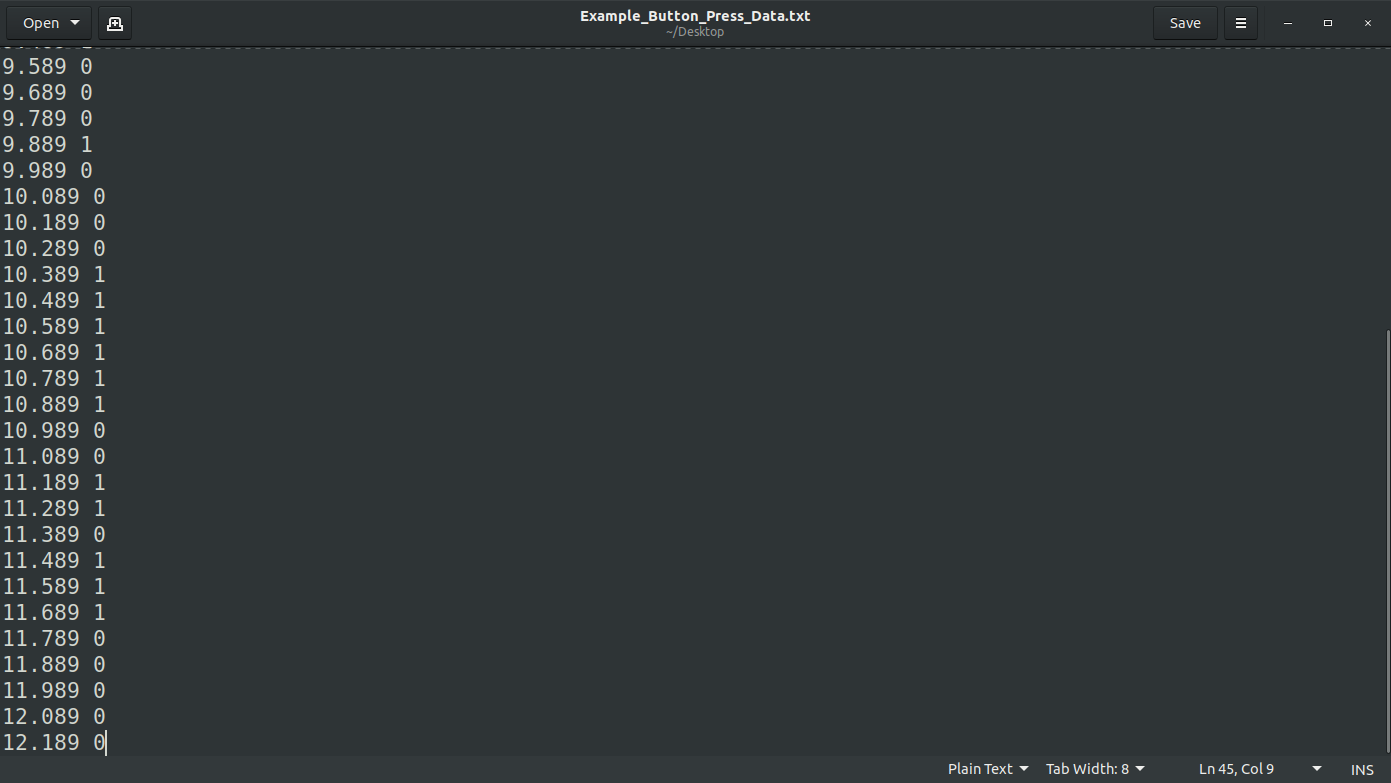
\includegraphics[width=\textwidth]{Figures/Gedit_Data.png}
  \end{center}
\end{figure}
At this point you can copy this text file over to your desktop computer and proceed to the Python plotting portion.
Ok so let’s recap method 3 one more time.
\begin{enumerate}[itemsep=-5pt]
\item Unplug CPX (or remove power)
\item Slide switch to A
\item Plug in CPX (or provide battery power)
\item Slide switch to B
\item Reset
\item Take data for however long you want
\item Slide switch to A
\item Remove power if you’re on battery power
\item Plug CPX into computer if not already connected
\item Transfer data file to computer
\end{enumerate}

\subsection{Plotting Logged Data}

Alright so there you have it. I have explained 3 methods to
datalogging. Here are the methods again in summary.

\begin{enumerate}[itemsep=-5pt]
\item Print data to Serial and copy and paste
\item Use the Keyboard module to save data to a spreadsheet
\item Access the storage of your CPX and write data to a text file on the CPX
\end{enumerate}

All methods will work but some will obviously have their pros and
cons. I suggest you get comfortable with 1 method and use that for the
remainder of the semester. Whatever option you choose though will
provide you with a data file that you can read in Python on your
desktop computer to plot. The simplest way to import data is by using
the loadtxt function from the module numpy. Here is some very simple
code to plot data from a text file. I also have a \href{https://www.youtube.com/watch?v=tJOz-ty-2ec&list=PL_D7_GvGz-v1RsDs_OdNW65qRjEjmpfQx&index=12}{Youtube video
explaining how to plot a text file} if you’d rather watch something. 

When you plot make sure your {\it Test\_Data.txt} file is in the same folder
as your plotting script in Thonny or Spyder. Here’s my example code
(this code is not on Github but you only need 3 or 4 lines of code to plot). 
\begin{figure}[H]
  \begin{center}
    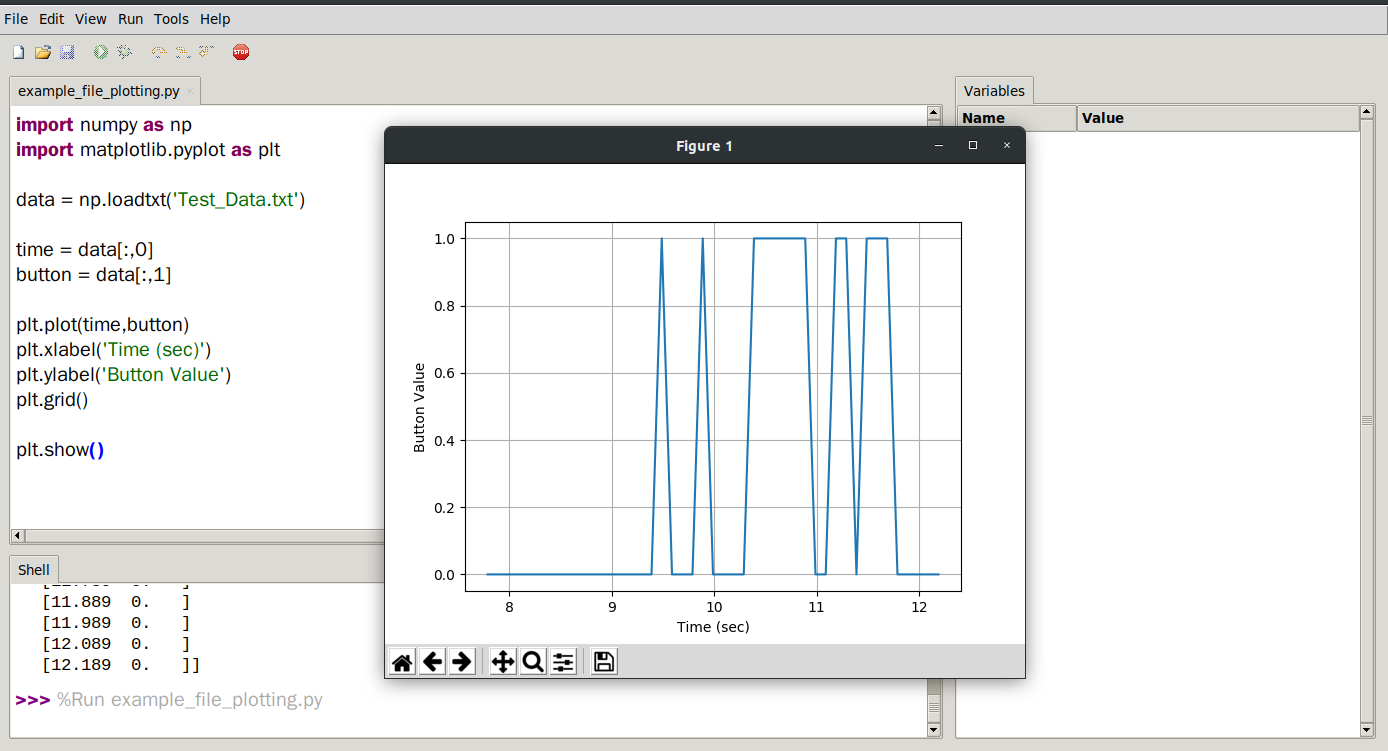
\includegraphics[width=\textwidth]{Figures/plotdata.png}
  \end{center}
\end{figure}
In this example lines 1 and 2 import numpy and matplotlib. Line 4
imports data from the {\it Test\_Data.txt} file and then 6 and 7 save the
first and second columns into time and button. The remaining lines
plot the data and create x and y labels as well as a grid. Hopefully
now you are well versed in taking data and plotting in Python.

\subsection{Assignment}

Upload a PDF with all of the photos and text below included. My
recommendation is for you to create a Word document and insert all the
photos and text into the document. Then export the Word document to a
PDF. For videos I suggest uploading the videos to Google Drive, turn
on link sharing and include a link in your PDF.
\begin{enumerate}[itemsep=-5pt]
\item Use method 1, 2 or 3 and save time and button presses to a text file
\item Include a video explaining which method you are using to record button presses and show yourself pressing the CPX button a few times and recording data. Make sure to wave and introduce yourself - 30\%
\item Copy and Paste your CPX code used to log data - 20\%
\item Copy and paste your Python desktop code used to plot your data - 20\%
\item Include a plot of your button presses with time on the x-axis and button presses on the y-axis (no screenshots) - 30\%
\end{enumerate}


\end{document}
